\documentclass[12pt]{book}
\usepackage{appendix}
\usepackage{graphicx}
\usepackage{mathtools}
\usepackage{xcolor}
\usepackage{enumitem}
\usepackage{multirow}
\usepackage{booktabs}
\usepackage[font=small,labelfont=bf]{caption}
\captionsetup[figure]{name=Fig.}
\parindent 0pt
\parskip 6pt
\def\rett#1{\texttt{\color{red}#1}}
\def\bltt#1{\texttt{\color{blue}#1}}
\def\grtt#1{\texttt{\color{magenta}#1}}
\graphicspath{{./figures/}}
\begin{document}
\frontmatter
\title{
piHPSDR User's Manual \\
\small{For development version 2.3}
}
\author{
Christoph van W\"ullen, DL1YCF \\
email: \texttt{dl1ycf@darc.de}
}

%
\maketitle
\textbf{Copyright Notice:}

Copyright (C) 2023 Christoph van W\"ullen, DL1YCF.

This work is licensed under
the Creative Commons licence CC BY-SA, version 4 or later, so it can be freely distributed.
 This license also allows reusers to distribute, modify and build upon the material in any medium or format,
as long as attribution is given to the creator. The license allows for commercial use.
If you modify or build upon the material, you must license the modified material under identical terms.

\textbf{Disclaimer.} The manual has been written with the intention that it is useful. It is quite clear
that it still contains errors, therefore it is stressed here that it comes without any warranty. The reader
is hereby explicitly warned that through wrong use of an SDR program such as piHPSDR, it is possible to
damage the radio hardware.

\textbf{Trade marks.} Registered trade marks are not marked with a sign in this manual. From the absence of
a trademark sign, it cannot be concluded that a mark you find in this manual is not registered or not
protected.

\bigskip
\textbf{The author:}

Christoph van W\"ullen (DL1YCF) has contributed a lot to piHPSDR in the last few years, this manual refers
to the code in his github account

\texttt{https://github.com/dl1ycf/pihpsdr}

where the \LaTeX\   ,,source code'' of this manual, together with all figures in .png format, can be found
in the \texttt{release/LatexManual} directory. At this moment this code has significant developed compared
to the piHPSDR code in John Melton's master repository, but there is still hope that both versions can
be merged in  the  future, although this  will  be hard  work.

If you think you can improve the manual, you are welcome.
Simply fork the above repository and make a pull request, or (this is the recommended way) write an
email to the author: \texttt{dl1ycf@darc.de}
\tableofcontents
\mainmatter
%%%%%%%%%%%%%%%%%%%%%%%%%%%%%%%%%%%%%%%%%%%%%%%%%%%%%%%%%%%%%%%%%%%%%%%%%%%%%%%%%%%%%%%%%%%%%%%%%%%%%%%%%%%%
\chapter{Introduction}
piHPSDR is a program that can operate with software defined radios (SDRs). As a graphical user interface,
it uses the GTK-3 toolkit, while the actual signal processing is done by Warren Pratt's WDSP library. Thus,
piHPSDR organizes the transfer of digitized radio frequency (RF) data between the radio hardware and the
WDSP library, the
transfer of audio data (either from a microphone or to a headphone), as well as the processing of user
input (either by mouse/touch-screen, keyboard, or external "knobs and buttons"),
 and the graphical display of the RF data. piHPSDR is intended
to run on different variants of Unix. It runs on all sorts of Linux systems, including a Raspberry Pi (hence
the name piHPSDR), but equally well on Linux desktop or laptop computers, and on Apple Macintosh (Mac OSX)
computers which have a Unix variant under the hood. The present author is not aware of piHPSDR running
under the Windows operating system, although with environments such as MinGW, this should be possible.

Although piHPSDR can be operated entirely by using mouse and keyboard as input devices, many users prefer to
have physical push-buttons and/or knobs or dials. To this end, piHPSDR can control push-buttons and rotary
encoders connected to the GPIO (general purpose input/output)
lines of a Raspberry Pi. At least two generations of such controllers have
been put on the market by Apache labs, and I know of several projects where home-brewn controllers have
successfully been made. As an alternative, MIDI devices can be used for user interaction. For desktop/laptop
computers that do not have GPIO lines, MIDI offers an easy-to-use possibility of having push-bottons and
dials that control piHPSDR. Apart from homebrew projects in which a micro-controller such as an Arduino
Micro controls the actual buttons/knobs and acts as a MIDI device to the computer to which it is connected
via USB, there are low-cost so-called "DJ controllers" (DJ stands for disk jockey) from various brands which
have successfully been used with piHPSDR. A third possibility to control piHPSDR is via a serial interface
through CAT (computer aided transceiver) commands. The CAT model used by piHPSDR is based on the Kenwood
TS-2000 command set with lots of PowerSDR extensions.

Using a touch-screen instead of a mouse offers the possiblity to put the actual radio hardware together
with a Raspberry Pi running piHPSDR and an assortment of buttons/knobs into a single enclosure. This way,
one can build an SDR radio which can be operated like a conventional analog one.

The piHPSDR program has been written by John Melton G0ORX/N6LYT. It is free software that is licensed under
the GNU (free software foundation) general public license. Many other radio amateurs have contributed to
the code. A lot of extensions and improvements have been added by myself, therefore this document refers
to the version of piHPSDR that can be found on my github account \texttt{https://github.com/dl1ycf/pihpsdr}.

Because piHPSDR can be used on many different types of computers, and because operating systems change
rather quickly over time, I generally do not recommend to do a ,,binary installation'' although such
a bundle is provided in the repository (for the RapsberryPi only) and the process is decribed in Appendix \ref{sec:installbinary}.
 Instead, my personal recommendation is to build piHPSDR
from the sources, only this procedure guarantees compatibility of the final program with your
operating system. Shell scripts for a semi-automatic installation have been provided,
and the procedure is described in Appendix \ref{sec:installsources} for Linux (including RaspPi)
computers and in Appendix \ref{sec:installmacosx} for Mac OSX.
This manual starts in its first chapter with the first invocation of a freshly compiled piHPSDR.

Within this manual, we shall use a typewriter font in red color if we refer to a text or a button within
a menu of within the VFO bar. piHPSDR menus and commands are indicated through a typewriter font
printed in blue. The author hopes that this improves readability. In some cases, if the name of a command
or  menu is written on the screen, you may find the same string both typed in red and blue in the
description, depending on whether the text refers to the command in an abstract sense or to the string as it
can be found on the screen. This may be confusing upon first reading, but I shall try to follow the coloring convention as laid out here.

%%%%%%%%%%%%%%%%%%%%%%%%%%%%%%%%%%%%%%%%%%%%%%%%%%%%%%%%%%%%%%%%%%%%%%%%%%%%%%%%%%%%%%%%%%%%%%%%%%%%%%%%%%%%
\chapter{Starting piHPSDR for the first time}
Let us assume you have an SDR (say, an ANAN-7000 or a HermesLite-II) powered up and connected to an antenna,
and you have piHPSDR installed on a computer (say, a Raspberry Pi or an Apple Macintosh), the first thing to
do is to establish a proper connection between the computer and the radio. Although advocated at many
places,
I do highly recommend against a WiFi connection. WiFi routers often use optimizations where they hold
back data packets for a given client for a while, to be able to send a collection of them in a burst. While
this certainly optimizes the through-put because it minimizes clear-channel arbitration events, such jitters
are desastrous in SDR operation. The safest way of connecting the radio and the computer is to have a
managed switch with a built-in DHCP server, and to connect both the computer and the radio with a suitable
cable to the switch. If the computer has both a RJ45 jack for an ethernet cable, and a WiFi interface, my
personal recommendation is to use WiFi to connect the computer to the internet, and use a single direct
cable plugged
into the RJ45 jacks of the computer and of the radio. This is a little bit tricky since both the computer
and the radio have to be set to a fixed IP address (e.g. computer: 192.168.1.50, radio: 192.168.1.51) with
the same netmask. However, once this has been done, this is the safest connection with no perturbations from
elsewhere.

\begin{figure}
\center
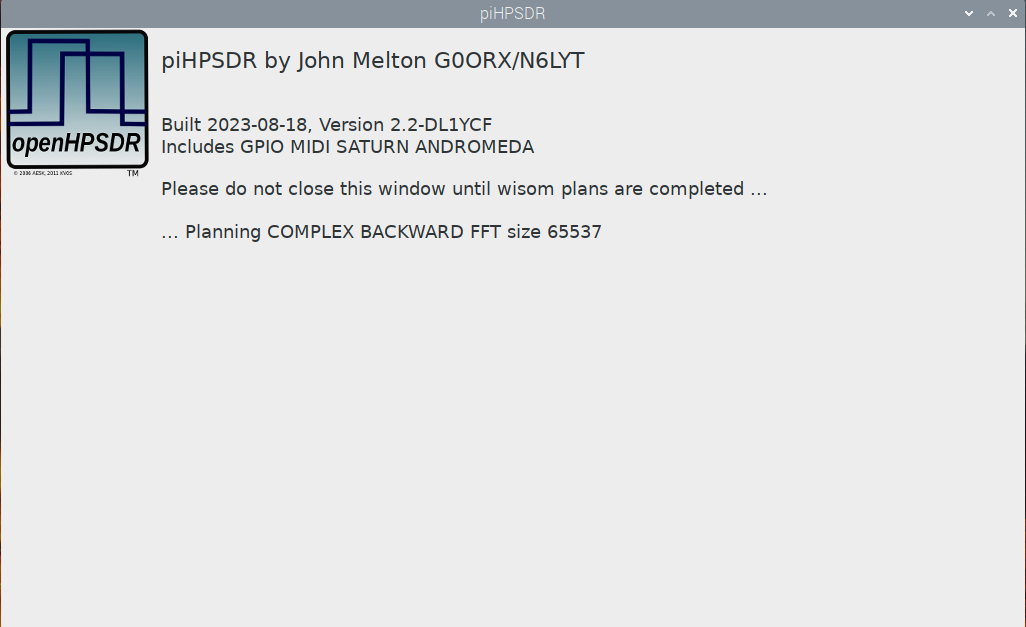
\includegraphics[width=12cm]{Planning.png}
\caption{piHPSDR screen while completing the \textit{wisdom plans}.}
\label{fig:Planning}
\end{figure}

If the piHPSDR program is started for the first time, it opens a window that looks like Fig. \ref{fig:Planning}.
Besides stating a version number and when piHPSDR was built, a list of optional features (to be activated
at compile time) is stated, in this case, GPIO, MIDI, SATURN. These are compile-time options that are
detailed in Appendix \ref{sec:compiletime}.

What is important here that you have to wait. This only applies to the very first time you start piHPSDR.
On CPUs with a rather simple instruction set (like the ARM processor in the Raspberry Pi, or the Apple
Silicon processor in recent Macintosh computers), this so-called  \textit{planning} step is quite fast. For
example, on my
Apple M2 Mac mini, this step only takes 6 seconds, and you have to wait for 34 seconds on a RaspberryPi 4.
On the contrary, on CPUs with
complex instruction sets, more planning is necessary: on my other Mac mini with a 3 GHz x86 processor, it
takes 16 minutes! But note
this has only to be done once, in subsequent starts of piHPSDR, the wisdom will simply be read from
the file created during the \textit{wisdom plans}. These plans contain, for a large number of dimensions,
the fasted way how to perform FFTs (fast Fourier transformations) on the given CPU.
When the wisdom is secured, piHPSDR tries to detect a radio on the network. If everything went well with
the network connection, you then see a screen with a discovery menu (Fig. \ref{fig:Start}).

\begin{figure}
\center
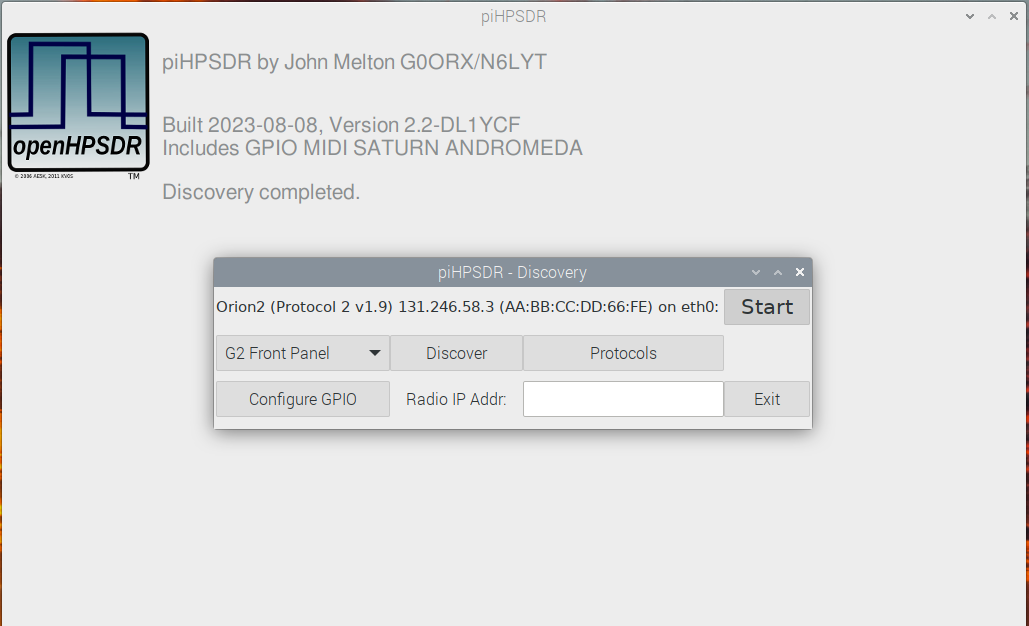
\includegraphics[width=12cm]{Start.png}
\caption{A radio has been discoverd. You are ready  to start it.}
\label{fig:Start}
\end{figure}

It is possible that the \rett{Start} button is deactivated and shows another text. \rett{In Use} at
this point means that the radio is already in use (connected by another SDR application), while
\rett{Incompatible} denotes that the radio is not compatible with this version of piHPSDR. This
is only the case if piHPDSR runs natively on the CM4 module inside the new Anan Saturn/G2
radios and the FPGA firmware is known to be too old for direct (XDMA) data transfer between the CM4
module and the FPGA. Updating the FPGA firmware to the latest version
should help in this case.

If more than one radio is available, or a radio can be connected via more than one network interface,
you will see several \rett{Start} buttons.
If you see at least one \rett{Start} button, you can start the corresponding radio simply
by clicking that button. But let us first explain the
purpose of the other buttons! Easiest to explain is the \rett{Exit} button, this will simply terminate
the program. Most likely, you may want to go into the \rett{Protocols} menu sooner or later.
By default, piHPSDR tries to discover the presence of a radio using all protocols known to piHPSDR. However,
if you know that your radio, for example, uses P2 (Protocol 2), then trying to discover a P1 (Protocol 1)
radio is just a waste of time. So if you know which types of radio you want to connect to, you can enable
(only) these in the \rett{Protocols} menu. The available protocols are

\begin{itemize}[font=\texttt, left=80pt]
\item[Protocol 1]{This is the "original" HPSDR protocol.}
\item[Protocol 2]{This is the "new" HPSDR protocol.}
\item[Saturn XDMA]{This is used to talk to a Saturn FPGA through the internal XDMA interface. Only available
if piHPSDR is compiled with the \texttt{SATURN}  option.}
\item[USB OZY]{This is used to talk to a radio using the legacy USB OZY interface. Only available if piHPSDR
is compiled with the \texttt{USBOZY} option.}
\item[SoapySDR]{This is used to talk to a radio through the SoapySDR library, for example to an AdalmPLUTO.
Only available if piHPSDR is compiled with the \texttt{SOAPYSDR} option.}
\item[STEMlab]{This is used to connect to RedPitaya based SDRs through the WEB interface. Only available if
piHPSDR is compiled with the \texttt{STEMLAB\_DISCOVERY} option. Starting the radio using this protocol is a
two-step process:
first, the RedPitaya's WEB interface is located, and the \texttt{Start} button then starts the SDR app
on the RedPitaya. Then, piHPSDR tries to connect to this SDR app and upon success offers a new
\texttt{Start} button to start the radio. If the RedPitaya is exclusively used as a radio, it is recommended
to auto-start the SDR app
when the RedPitaya is powered up. In this case, the STEMlab protocol is not used, because the SDR app can be started through Protocol-2.}
\item[Autostart]{This is a very useful option. It indicates that if exactly one radio has been found, it is
automatically started. So in normal operation, when starting piHPSDR subsequently, and all settings are
still valid, the radio is started without user intervention. If this option is activated and one radio is
present, you will not see this menu, so in order to make further changes here, you have to disconnect the
radio from the ethernet cable, start piHPSDR until you see this menu, and update the \rett{Protocols}
settings. Then you can re-discover using the \rett{Discover} button.}
\end{itemize}

Sometimes piHPSDR needs to know the IP address of the radio. This is, for example, the case for the
\texttt{STEMlab} discovery
described above. In such a case the IP address in numerical form (xxx.xxx.xxx.xxx) can be entered in the box
with the label \rett{Radio IP Addr:}. If a legal IP address is contained in this box, protocol-1 and
protocol-2 discoveries
will also send to the IP address specified, in addition to the standard broadcast discovery packets which
can only reach
radios on the same network segment. With a known IP address,  one can
connect to radios which are not on the same subnet as the computer, in principle you can connect to any
radio on the world
provided it is on the internet. However, the original HPSDR standard states that a broadcast packet must be
used, so several
radios won't reply. On the other hand, there are some radios such as a RedPitaya or a HermesLite-II which
allow being discovered by such a routed packet.

The \rett{Discover} button re-starts the discovery process. This is useful if the radio has been powered up
too late and
was not yet ready when piHPSDR was started. Simply press \rett{Discover} to start another attempt.

The combo-box (pop-down menu) to the left of the \rett{Discover} button lets you choose which type of GPIO
controller you
have attached to the computer. This menu is only available if piHPSDR has been compiled with the
\texttt{GPIO} option, which
is not the case on desktop/laptop computers. The menu lets you choose between

\begin{itemize}[font=\texttt, left=80pt]
\item[No Controller]{Choose this if no GPIO controller is wired to your Raspberry Pi. This is the default
when you first start piHPSDR.}
\item[Contoller1]{Choose this if you have the original piHPSDR controller, called the Controller1 in the rest
of this manual.}
\item[Controller2 V1]{This option is valid for some early prototypes of the "version 2" controller with
single encoders. This special case is not covered in this manual.}
\item[Controller2 V2]{Choose this if you have a "version 2" piHPSDR controller with double encocders.
This controller is denoted Controller2 in the rest of this manual.}
\item[G2 Front Panel]{Choose this if you have an ANAN G2 radio with a built-in controller.}
\end{itemize}

\textbf{Attention.} Be sure to choose a controller only if such a controller is actually connected to your
Raspberry Pi. If
you choose, for example, a controller which uses an I2C expander for the switches, but no I2C interface is
present on
your Raspberry Pi, the program my hang when trying to open the I2C connection.

All settings (protocols, controller, IP address) made in this menu are stored in the global (radio-
indepentend) settings
and are restored when piHPSDR is started the next time.

If all went well, a radio could be discovered and you hit the \rett{Start} button, the radio is started, and
if this succeeds, you see something like shown in Fig. \ref{fig:FirstDisplay}.

\begin{figure}
\center
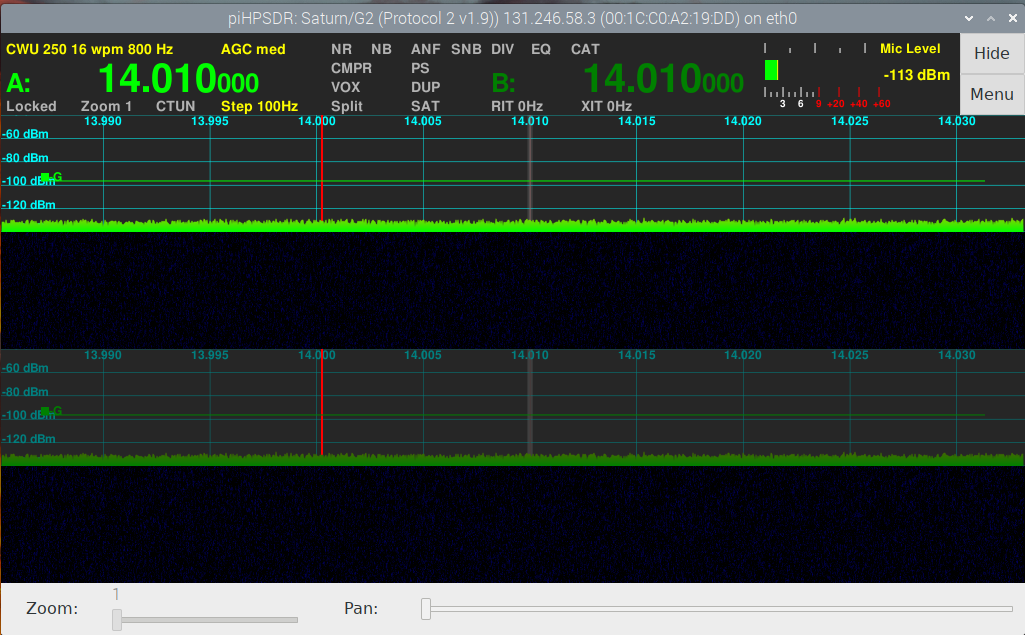
\includegraphics[width=12cm]{FirstDisplay.png}
\caption{The radio with two RX. Sliders and Toolbar are not on display
by default when using a controller.}
\label{fig:FirstDisplay}
\end{figure}

The bottom of the window looks different (more controls) if you have chosen \rett{No Controller} in the
preceeding menu.
You see two receiver panels stacked vertically, both of them having a spectrum display and a waterfall area.
At the top,
just below the window title, you have the VFO bar which contains information on the frequencies of the two
VFOs A and B,
as well as lots of further information, to be explained later. At the top right, there are two buttons
\rett{Hide}
and \rett{Menu} which will be explained in the next chapter. To the left of these two buttons, there is the
meter bar which by default is a digital S-meter. At this point, you have started piHPSDR successfully for
the first time.

%%%%%%%%%%%%%%%%%%%%%%%%%%%%%%%%%%%%%%%%%%%%%%%%%%%%%%%%%%%%%%%%%%%%%%%%%%%%%%%%%%%%%%%%%%%%%%%%%%%%%%%%%%%%
%%%%%%%%%%%%%%%%%%%%%%%%%%%%%%%%%%%%%%%%%%%%%%%%%%%%%%%%%%%%%%%%%%%%%%%%%%%%%%%%%%%%%%%%%%%%%%%%%%%%%%%%%%%%
\chapter{Main window layout}

\section{One or two receivers}
At the end of the previous chapter (Fig. \ref{fig:FirstDisplay}),
 there were two receiver panels in the
piHPSDR window, stacked vertically, and both including a spectrum scope
(the green-coloured noise floor) and a waterfall. The waterfall area
is completely black in the above picture since there was no RF signal.
piHPSDR can be switched between having one or two receivers in the
\texttt{Radio} menu. If there are two receivers (called RX1 and RX2),
 one of the two is the \textit{active receiver}. If you look closely
 at the above picture, you will note that the spectrum scope of
 the lower (RX2) panel is shaded, while it is in bright colour for RX1.
 This indicates that RX1 is currently the active receiver. By simply
 clicking into the panel of the other (inactive) receiver, either with
 a mouse or on a touch screen, the formely inactive receiver becomes
 active.

 Many conventional rigs with two independent receivers discriminate
 between the \textit{main} and the \textit{sub} receiver. It is important that
 this is \textbf{not} the case for piHPSDR. In piHPDSR, both  receivers are
 largely equivalent. For example, if you start transmitting in
 normal (non-split) mode, the TX frequency matches the frequency
 of the active receiver, no matter whether this is RX1 or RX2.
 Likewise, in split mode, the TX frequency matches the frequency
 of the non-active receiver. Most of the receiver-specific controls,
 for example adjusting the AF volume or the AGC gain, refer to the
 current active receiver. If piHPSDR runs with two receivers,
 RX1 is always controlled by VFO-A while RX2 is controlled by VFO-B.
 The VFO settings not only include the frequency but also the
 current mode (e.g. LSB or CWU), the filter setting, the band and
 bandstack setting, whether RIT is enabled or not, and the RIT
 offset. So changing the RIT value only changes it for the active
 receiver. If you want  to change the RIT value for RX2 while RX1 is
 the active receiver, you have to make RX2 active, change the RIT
 value and then make RX1 active again.

 RX1 and RX2 are largely independent. They can receive on different
 bands. They can receive from different antennas provided the radio
 has two RF frontend with two analog-to-digital converter4s (ADC,
 as most modern radios do. In this case, one usually
 assigns the first ADC (ADC0) to RX1 and the second ADC (ADC1) to
 RX2. This can be done in the \bltt{RX} menu.

 By default, if there are two receivers, they are vertically stacked,
 with RX1 in the upper part and RX2 in the lower part of the display.
 This can be changed in the \bltt{Screen} menu to horizontal stacking,
 where RX1 is  in the left half and RX2 in the right half of  the
 display. Changing the stacking trades vertical against horizontal
 resolution, of course.


\begin{figure}[ht]
\center
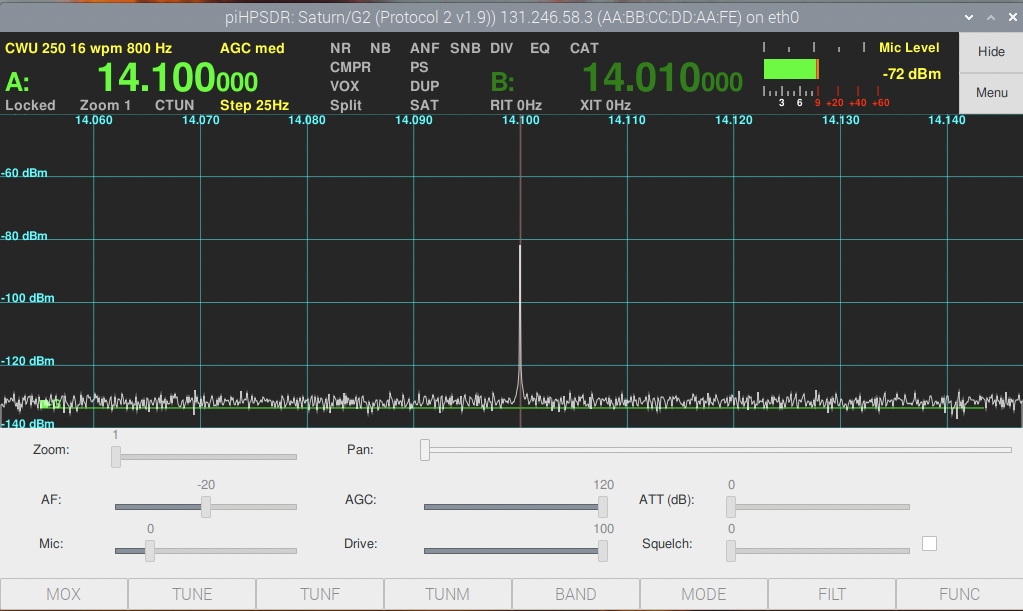
\includegraphics[width=12cm]{SingleReceiver.png}
\caption{piHPSDR with a single RX and all controls (Zoom/Pan,
Sliders, Toolbar) at the  bottom.}
\label{fig:SingleReceiver}
\end{figure}

 Fig. \ref{fig:SingleReceiver} picture shows, for demonstration purpose, a piHPSDR
 window with a single receiver.
 The RX panel only contains a
 spectrum scope with a white line and no waterfall (this can be changed in the
 \bltt{Display} menu. In addition, you see the toolbar
 with eight buttons at the lower edge of the window, and above
 it an area with sliders. Showing the sliders is the default
 (and necessary) if there is no GPIO or MIDI controller attached,
 since then these sliders are the only way to change, for example,
 the AF volume. If there is only one receiver, it is controlled
 by VFO-A. VFO-B then actually controls nothing (except the TX
 frequency in split mode), but the data stored in VFO-B can
 be quickly used, for example by copying VFO-B to VFO-A (the
 \bltt{A<B} command), or by swapping the two VFOs (the \bltt{A<>B} command).

%%%%%%%%%%%%%%%%%%%%%%%%%%%%%%%%%%%%%%%%%%%%%%%%%%%%%%%%%%%%%%%%%%%%%%%%%%%%%%%%%%%%%%%%%%%%%%%%%%%%%%%%%%%%
\section{Spectrum scope options}
\label{sec:FillingGradient}

You have already seen two different spectrum scopes: in the first
picture, the  spectrum was a filled green area, while in the last
picture, there only was a white line (this is similar to what you
would see on a spectrum analyzer). This can be adjusted to your
personal preference in the \bltt{Display} menu (see below). There
are two options which you can enable or disable, such that there
are four different outcomes. The first option is the ,,Filled'' option
which discriminates between a line spectrum and a spectrum which is
filled below the line. In the picture below, the first and third
example have no filling, while the second and fourth spectrum
are filled:

\begin{figure}[ht]
\center
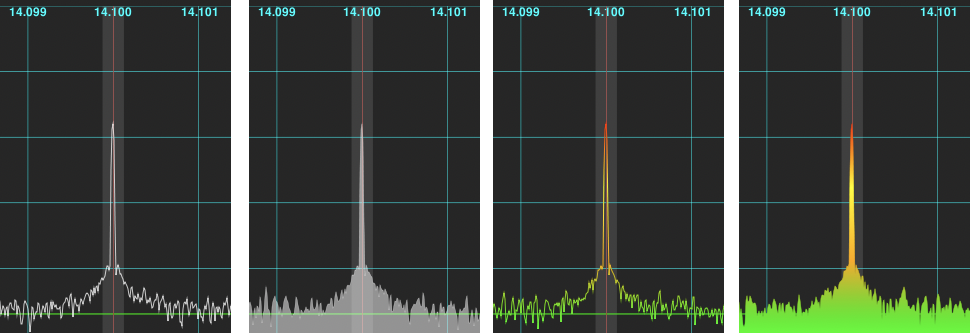
\includegraphics[width=12cm]{ScopeFilling.png}
\caption{Display options for the spectrum scope.}
\end{figure}

Then there is the ,,Gradient'' option. Without this option, the
spectrum is displayed in white colour. With the gradient option,
the colour changes from green over yellow towards red depending
on the signal strength (red colour is reached for S9). The above
picture demonstrates the four possible combinations, and in
the \bltt{Display} menu, you can make your choice. This setting
refers to both receivers when there are two. Note that the TX
spectrum can be a filled one or a line spectrum, but that the
gradient option does not apply.

%%%%%%%%%%%%%%%%%%%%%%%%%%%%%%%%%%%%%%%%%%%%%%%%%%%%%%%%%%%%%%%%%%%%%%%%%%%%%%%%%%%%%%%%%%%%%%%%%%%%%%%%%%%%
\section{Zoom and Pan}

\begin{figure}[ht]
\center
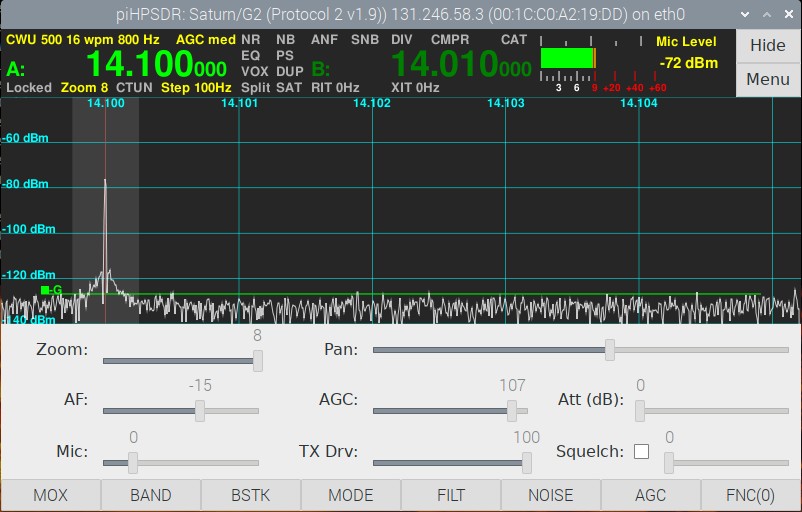
\includegraphics[width=12cm]{ZoomPan.png}
\caption{The spectrum scope of Fig. \ref{fig:SingleReceiver} with a
large Zoom value.}
\end{figure}

The width of the RX spectrum equals the sample rate
of the receiver. This means that if you use, say,
a sample rate of 96 kHz for a receiver, its spectrum
will be 96 kHz wide, which may encompass a larger part
of the spectrum than you are interested in. As a drawback,
the part which is relevant to you may look a little bit
compressed. This is where the \bltt{Zoom} command
comes in. The zoom value can adopt integral values between
1 (no zoom) and 8. In the latter case, only 1/8 of the
overall spectrum is displayed on the screen. In the
picture below, you see that the RX scope is only 12 kHz
wide (which is 1/8 of the RX sample rate, 96 kHz in our
example). Note that what is displayed is in full resolution.
Internally, a spectrum with 8 times the number of pixels
of the screen width is created and only a part of it is
displayed. The zoom value can be changed using the \rett{Zoom}
slider (at the left edge below the RX panel).


When using a zoom value larger than one, this means that
a spectrum with more pixels than the actual screen width
is produced. One can select which part of that area
is displayed on the screen with the \rett{Pan} slider
(below the RX panel at the right side). Normally (Zoom=1),
the VFO dial frequency is exactly in the middle of the
RX scope, and marked with a thin red line. On the picture
above, the dial frequency (14.100 MHz) is found in the RX
panel close to the left edge, and this has been done
by moving the \rett{Pan} slider.

%%%%%%%%%%%%%%%%%%%%%%%%%%%%%%%%%%%%%%%%%%%%%%%%%%%%%%%%%%%%%%%%%%%%%%%%%%%%%%%%%%%%%%%%%%%%%%%%%%%%%%%%%%%%
\section{The \texttt{Hide} button}
\begin{figure}[ht]
\center
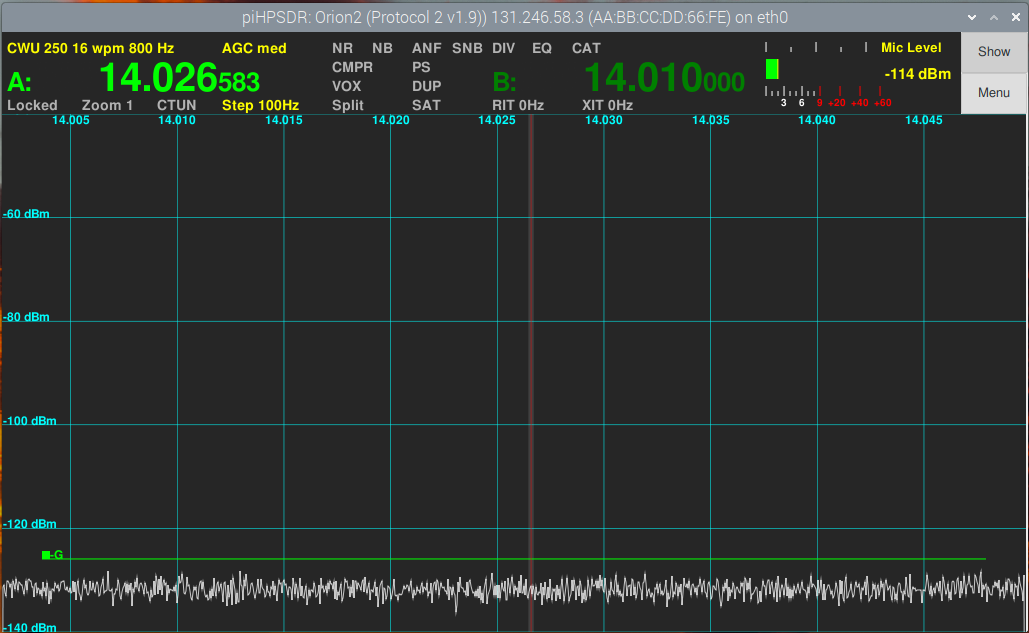
\includegraphics[width=12cm]{Hidden.png}
\caption{piHPSDR window with the Toolbar/Sliders/Zoom
area ,,hidden''.}
\end{figure}

On small screens, space is scarce. This in in particular true
for the vertical space if one used two RX panels and both
with a spectrum scope and a waterfall. I this case, it may be
hard to actually watch the signals if the screen is small.
This is where the \rett{Hide} button comes in. Clicking on
this button ,,hides'' the toolbar and slider area:


The text on the button then changes to \rett{Show}, and
clicking this button again will then return to the
previous display.

%%%%%%%%%%%%%%%%%%%%%%%%%%%%%%%%%%%%%%%%%%%%%%%%%%%%%%%%%%%%%%%%%%%%%%%%%%%%%%%%%%%%%%%%%%%%%%%%%%%%%%%%%%%%
\section{Window areas}

Look again at Fig. \ref{fig:SingleReceiver}! Starting from the
top, you see the title bar of the window. This bar is not visible
in full screen mode, where the size of the piHPSDR window matches
the display size. The title bar contains some basis information
about the radio, e.g.  its type, the protocol used, the  IP
and the hardware address of the radio. If you are really interested
in this information, it is recommended to open the
\bltt{About} menu.

Between the title bar and the RX spectrum scope, you see
a small vertical area, most of  which is taken by the VFO bar
(containing the large frequency dials). At the rightmost
end of this area, you see two buttons \rett{Hide} (already
discussed) and \rett{Menu}. Clicking on the latter button opens
the main menu, which will be discussed in detail in the following
chapters. The \rett{Menu} button is really important, since it
enables access to one of the menus used for configuring piHPSDR.
Between the VFO bar and the \rett{Hide}/\rett{Menu} buttons,
you see the meter area where you find the S-meter (during RX)
and information about output power, SWR, etc. during TX.

Below the RX  spectrum scope, you see the Zoom/Pan area with
the  Zoom and Pan sliders, as already discussed. This area
can be ,,hidden'' with the \bltt{Display} menu to save some
vertical space. Below the
Zoom/Pan sliders you see a larger  Sliders area containing
several sliders for adjusting AF volume, TX  drive level,
RX  AGC threshold, etc. Although the Sliders area can also
be hidden via the \bltt{Display} menu, you should not do so
unless you have a GPIO or MIDI controller which knobs that
you can asssign to the slider functions. This is so since
for  normal operation, having access to the sliders is vital.
Remember that for temporarily enlarging the space for
the RX  panel, there is the \rett{Hide} button!

\begin{figure}
\center
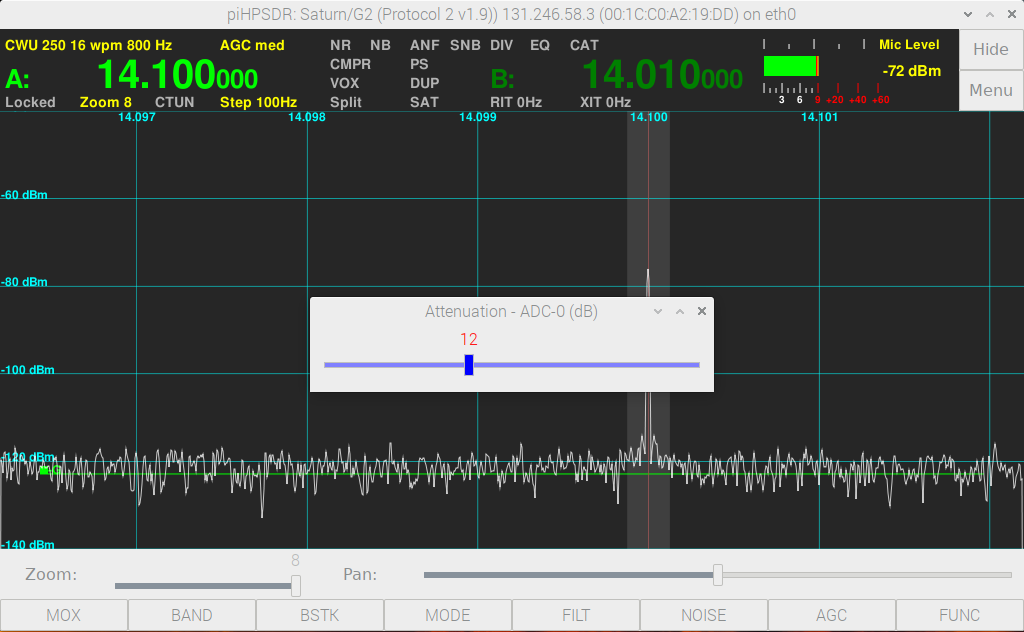
\includegraphics[width=12cm]{SliderOnScreen.png}
\caption{A pop-up attenuation slider.}
\label{fig:SliderOnScreen}
\end{figure}

If you have a GPIO or  MIDI  console, and, say, assigned
a knob there to control the AF volume, then turning the
knob will auto-magically also move the AF slider if its
on display (that is, if the sliders area is not hidden).
If you turn a knob for which function there is slider
on display, either because the slider area is hidden or
because this function does not have a slider in that area,
then a graphical slider will temporarily pop up in the
middle of the window to inform you about the changes
you have  made. To give one example, a knob at a
MIDI console has been assigned to the RF attenuator (\bltt{Atten}
function, see Appendix A), which controls the step
attenuator in the RF front-end (if there is one). As long
as the  sliders  are  on display, the \rett{Att} slider
in the right part of the slider area moves when turning
the knob. But when the sliders are not displayed, then a slider image
pops up  on the middle of the screen, and the
bar contained therein moves when turning the knob,
and the numerical value is displayed as well (Fig. \ref{fig:SliderOnScreen}).
Such a pop-up slider always occurs if a knob on the GPIO or MIDI
console is turned and no slider associated with the value changing is
on display.

At the very bottom of the window, there it the toolbar. This can also be
individually hidden/shown via the \bltt{Display} menu. The toolbar consists
of eight ,,buttons'' which you can click with a mouse or on a touchscreen.
If you are using the original (V1) piHPSDR GPIO controller, is has eight
push buttons below the screen and pressing those is equivalent to clicking
the buttons on the screen. You might still want to keep the toolbar on display
even if you are using the Controller1 since it shows you to which functions
the buttons are actually assigned. This assignments consists of six ,,layers''
(0 through 5). The rightmost button is hard-wired to the \bltt{Function}
action which cycles through the layers. The button text includes the
number of the currently active layer, and the button text of the other buttons
reflect the functions assigned to the buttons in the current layer.

\textbf{Bonus for mouse users only.} For the first seven toolbar buttons,
there is no difference if you do a primary or secondary mouse click on that
button (that is, it does not matter whether you use the left or right mouse
button). But for the rightmost toolbar button, a normally mouse click cycles
forward through the layers, while a secondary mouse click cycles backwards.
If you use a V2 or G2-frontpanel GPIO controller or a MIDI console, then you
can also map this function (\bltt{FuncRev}) to a spare button.


%%%%%%%%%%%%%%%%%%%%%%%%%%%%%%%%%%%%%%%%%%%%%%%%%%%%%%%%%%%%%%%%%%%%%%%%%%%%%%%%%%%%%%%%%%%%%%%%%%%%%%%%%%%%
\section{Mouse clicks in the main window}
The main window ,,accepts'' mouse or touchscreen click events.
Some of them come from the standard handlers of the GUI. It is
clear, for example, that clicking the \rett{Hide} or
\rett{Menu} buttons, as well as clicking one of the
toolbar buttons, will activate the function associated with
these buttons. Furthermore, the sliders (and the squelch enable/disable
checkbox) in the sliders and Zoom/Pan are are operated as usual.
But there are additional functions coded into piHPSDR:

If there are two receivers, a mouse click (press and release) into
the panel of the non-active receiver makes it active. On the other
hand, a mouse click in the panel of the active receiver changes
the VFO frequency of that receiver to the value clicked on.
This means, if you see a signal in the spectrum scope, click
on that signal and your VFO will move (\textit{jump}) to that signal.
Note the VFO frequency will be  rounded to the next multiple of
the VFO step size when jumping by a mouse  click or
touch screen press.

The second option to change the VFO frequency of the active receiver
is to click (and hold) into its panel, then drag the mouse to the left
or to the right, and then release the button. This will shift the
VFO frequency by the amount dragged, it makes no difference
where the first click actually occured, only the difference
in horizontal position between click and release is used. You must
drag at least three pixels so there is clear discrimination between
a ,\textit{VFO jump} (click then release) and a \textit{VFO drag} (click, drag,
and release) operation. Finally, the VFO frequency of the active
receiver can be changed by the scroll wheel of the mouse, if there
is any. Using the scroll wheel lets the VFO frequency move in multiples
of the VFO step size, while mouse dragging can also be used for
finer tuning.

Clicking into the VFO bar opens the \bltt{FREQ} (VFO) menu,
for the VFO-A if clicked into the left half of the bar, and for
VFO-B if clicked into the right half. This menu not only offers
the possibility for direct frequency entry, but also lets you
alter the RIT/XIT or VFO step size, or alter the Lock, Duplex,
CTUN, or Split states. So a simple click in the VFO bar
gets you quick access to often-used functions.

Clicking in the meter section (between the VFO bar and the
Hide/Menu buttons) opens the \bltt{METER} menu, where
you can change the meter properties (see below).

When operating with a mouse, there are usually two mouse buttons,
the primary button (for right-handed mouses, this is usually
the left button) and a secondary one. Secondary mouse clicks
are difficult to apply with a touch-screen. Although there are
touch-screen drivers which convert long presses to secondary clicks,
they generate, for a long press, a primary click first and a
secondary one later, so it is not possible to generate a
single ,,secondary press'' event. But for the benefit of
mouse users, secondary mouse clicks are handled in a special way:

A secondary click into the VFO bar will open the \bltt{BAND} menu,
so a band change can be made with really few mouse clicks. Likewise,
a secondary click into the panel of a receiver (no matter if it
the active or the non-active one) will open the \bltt{RX} menu
for that receiver. This can be used to change the settings of a
non-active receiver without making it temporarily active. In the
same way, a secondary click in the TX panel will open the
\bltt{TX} menu.

%%%%%%%%%%%%%%%%%%%%%%%%%%%%%%%%%%%%%%%%%%%%%%%%%%%%%%%%%%%%%%%%%%%%%%%%%%%%%%%%%%%%%%%%%%%%%%%%%%%%%%%%%%%%
\section{VFO bar and status  indicators}
\label{sec:VFObar}
\begin{figure}[ht]
\center
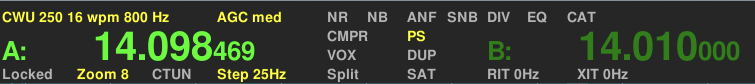
\includegraphics[width=12cm]{VFObar.png}
\caption{The VFO bar}
\label{fig:VFObar}
\end{figure}

Fig. \ref{fig:VFObar} shows the VFO bar layout in more  detail.
The example shown is a VFO bar whose width is 745 pixels and
thus suitable for screens that are 1024 pixels wide (or more),
since the meter area has a fixed width of 200 pixels, and
the \rett{Hide}/\rett{Menu} buttons are 65 pixels wide. This layout is
denoted \texttt{Large dials for 1024px windows}, as to the choice
of VFO bar layouts, see the description of the \bltt{Screen} menu.

The large dials indicating the frequencies of VFO-A and VFO-B
are easily recognized. The number to the left of the decimal
point is the MHz part of the frequency, the three  large digits
to the right  of  the decimal point is the kHz part, and
the last three (smaller) digits offer sub-kHz resolution.
You may wonder why there is  so much space to the left of
the frequencies. This is so because with the advent of
the QO-100 satellite, frequencies above 10 GHz can be
used (with the transverter bands) and therefore eleven
digits are needed!

Apart from the frequencies, you see a lot  of text, most in
light grey colour. As a general rule, a text  in grey
colour indicates a feature that is currently disabled,
while features currently active are normally shown in
yellow and sometimes in red.

At the top left  corner of the VFO bar, the mode and
filter of the currently active receiver is displayed.
In Fig. \ref{fig:VFObar}, the text is \rett{USB Var1}
which indicates that the  mode
is USB using the Var1 filter with variable width (see the \bltt{Filter} menu).
For the CW (CWU and CWL) modes, the CW speed (in wpm) and the side tone
frequency (in Hz) is stated as well. For CW, the filter size may be appended
by a ,,P'', which indicates whether the CW audio peak filter (see the
\bltt{Filter} menu) is effective on top of the normal filter.
For the FMN mode, an indicator of the form C=xxx.y is added if
CTCSS is enables, and then xxx.y shows the CTCSS frequency.

Now we continue line by line, from left to right and find
the string \rett{AGC med} printed in yellow. This means
that automatic gain control (AGC)  is effective  in the
active receiver, and that the AGC time constant is
intermediate. Possible values for the time constant
are Long, Slow, Medium and Fast which can be selected
in the \bltt{AGC} menu. Here one can  also disable AGC,
in this case the VFO bar shows \rett{AGC off} in grey
colour.

Continuing to the left, we see the noise reduction settings,
all printed in grey (that is, they are not effective). This
can be changed in the \bltt{Noise} menu. We have two different
noise reduction capabilities \rett{NR1} and \rett{NR2}, these
strings are printed in yellow instead of the grey \rett{NR} if
they are effective. There are also two different noise blankers
\rett{NB1} and \rett{NB2}, the automatic notch  filter
\rett{ANF} and the spectral  noise blanker \rett{SNB}.
Besides enabling/disabling these functions, there are  further parameters
you can tweak in the \bltt{Noise} menu.

The next strings whether Diversity reception is enabled or disabled
(\rett{DIV}), or whether an equalizer is effective \rett{EQ}.
Since there is a separate equalizer for the RX and TX audio chain,
the equalizer indicator, if it is effective, not only turns yellow
but reads \rett{RXEQ} while receiving and \rett{TXEQ} while
transmitting. This means, if only the TX equalizer is enabled,
the indicator will show a  grey \rett{EQ} while receiving
and a yellow \rett{TXEQ}  while  transmitting.

The last indicator in the top row  is \rett{CAT} which indicates
if the CAT module  (see the \bltt{RIGCTL}  menu) has accepted at least
one connection. In total, piHPSDR can be CAT-controlled simultaneously
by five different sources, two of them using a serial line and
three of them a TCP connection.

The indicators in the middle, between the VFO dials, are related to
transmitting. \rett{CMPR} indicates if a speech processor
(compressor) is enabled, if so, it prints in yellow, followed
by a number between 1 and 20 indicating the compression value in dB.
\rett{PS} indicates whether adaptive pre-distortion (,,PureSignal'')
is enabled, PS settings can be made in the \bltt{PS} menu.
 \rett{VOX} indicates whether VOX (voice control) is enabled. VOX means
 that if  the microphone delivers an amplitude above a certain threshold,
 the radio is automatically put into TX mode. Enabling/Disabling VOX
 and setting the correct threshold can be done in the \bltt{VOX} menu.
 Finally, \rett{DUP} indicates whether duplex mode is active.
 In duplex mode, the receiver(s) continue to work during transmit. Duplex
 mode when using the same antenna for RX and TX is  no fun: you not only hear
 your own signal with a delay (from the cross-talk at the TRX relay), but
 this cross-talk signal is  usually so strong that it leads to ,,AGC pumping'', so
 your receiver is virtually deaf during the first second after TX/RX
 transition. For satellite operation, on the other hand, duplex  mode
 is very convenient. Here you usually have two separate and well-decoupled
 antennas for RX and TX.

 The bottom line of the VFO bar  indicators are related to the VFO status.
 If the \rett{Locked} string is red, it indicates that the VFO is locked
 and will not accept changes. There is a LOCK action which toggles the
 LOCK status and which can be assigned to a toolbar button or a push-button
 on a GPIO or MIDI console, but the Lock status can also be set/unset
 via the \bltt{FREQ} menu, accessibly by the main menu window, or just by
 clicking into the VFO bar.

The next indicator in the bottom  line indicates the Zoom factor. If the
Zoom factor is 1, the indicator is grey, otherwise it is yellow and
also indicates the factor. Then there is a string \rett{CTUN} which
indicates whether the CTUN (,,click to tune'') mode is off or on (the string
is yellow in the latter case). The step size of the VFO controlling the
active receiver is displayed next, this string is always yellow.

The split status is displayed by the next indicator, which is red in
split mode. If split mode is off, transmitting is done on the frequency
and the mode of the active receiver (if there are two receivers), or
on the frequency/mode of VFO-A (if there is only one receiver). If
split mode is on, transmitting occurs on the frequency/mode of the
non-active receiver (if there are 2) or on VFO-B (if there is only  one
receiver).

The next indicator shows the SAT (satellite) mode, which can be off
(then the indicator reads \rett{SAT} in grey), or which can be SAT or RSAT
(then the indicator displays this string). Once SAT mode is engaged,
the two VFOs are tied together such that any frequency change of one
of the two VFOs also applies to the other VFO. This is the best way
to do cross-band operation with, e.g. the QO-100 satellite which is at
a fixed position. In RSAT mode, a frequency change of one of the VFOs
is applied to the other VFO with an opposite sign (so if you move up
VFO-A by 2 kHZ, then VFO-B moves down by the same amount). This is
what one needs for low-flying satellites which have inverting
transponders which offer some sort of Doppler correction.

Finally there are the \rett{RIT} (receiver incremental tuning) and \rett{XIT}
(transmitter incremental tuning) indicators. If RIT is off,
receiving occurs on the VFO dial frequency. If RIT is on, the
indicator becomes yellow and also indicates the RIT offset, that is,
the frequency offset used while receiving. RIT is used, for example,
if during your CW QSO the frequency of the transmitter of your
QSO partner drifts and you want to follow without altering the
frequency of your own transmitted signal. The RIT indicator
corresponds to the active receiver. If XIT is active, the
indicator becomes yellow and shows the offset of the true
TX frequency from the VFO dial frequency.

Finally, in the top right corner you see a symbol with a green and a red line
that only occurs if
one of the variable filters (\texttt{Var1} or \texttt{Var2}) have been
selected. The green caret indicates the default filter edges,  while the
red one above denotes the current filter edges.

%%%%%%%%%%%%%%%%%%%%%%%%%%%%%%%%%%%%%%%%%%%%%%%%%%%%%%%%%%%%%%%%%%%%%%%%%%%%%%%%%%%%%%%%%%%%%%%%%%%%%%%%%%%%
\section{Meter section}
\label{sec:MeterSection}
Fig. \ref{fig:MeterDesigns} shows the different designs that exist for
the meter. To the left (right) there are the digital (analog) meters,
while the top panels show the meter during RX and the lower panels
during TX.

\begin{figure}[ht]
\center
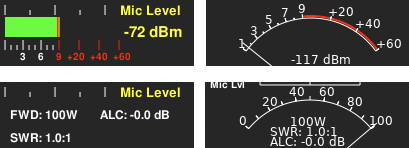
\includegraphics[width=8cm]{MeterDesigns.png}
\caption{Different designs for the meter.}
\label{fig:MeterDesigns}
\end{figure}

The design can be switched between digital and analog in the \bltt{Meter}
menu, which can be accessed quickly just by clicking into the meter area.
During RX, an S-meter is shown together with the signal level in dBm. Note
that -73 dBm corresponds to S9 for frequencies up to 30 MHz, while above
30 MHz, S9 corresponds to -93 dBm. Since the S meter is in steps of
6 dB, a signal level of S1 (below 30 MHz) corresponds to -121 dBm.

During TX, the output power is displayed, provided that the radio actually
reports this power. The output power meter can be calibrated (see the \bltt{PA}
menu). If the SWR exceeds a threshold for SWR warnings (the default is 1:3, but
this can be changed in the \bltt{TX} menu), the SWR indicator turns red. If,
in addition, SWR protection is enabled in the \bltt{TX} menu, the output
drived  will be reduced to zero if the SWR exceed that threshold.
Furthermore, the ALC (automatic level control) value of the transmitter is
shown. Negative ALC values (at least in peak mode) indicate that the volume of the TX input audio
could be increased to get full output  power.

Further info on the meters (e.g. switching between ,,peak'' and ,,average'' reporting)
is described in the \bltt{Meter} menu.

%%%%%%%%%%%%%%%%%%%%%%%%%%%%%%%%%%%%%%%%%%%%%%%%%%%%%%%%%%%%%%%%%%%%%%%%%%%%%%%%%%%%%%%%%%%%%%%%%%%%%%%%%%%%
%%%%%%%%%%%%%%%%%%%%%%%%%%%%%%%%%%%%%%%%%%%%%%%%%%%%%%%%%%%%%%%%%%%%%%%%%%%%%%%%%%%%%%%%%%%%%%%%%%%%%%%%%%%%
\chapter{The Main Menu: introduction}

\begin{figure}[ht]
\center
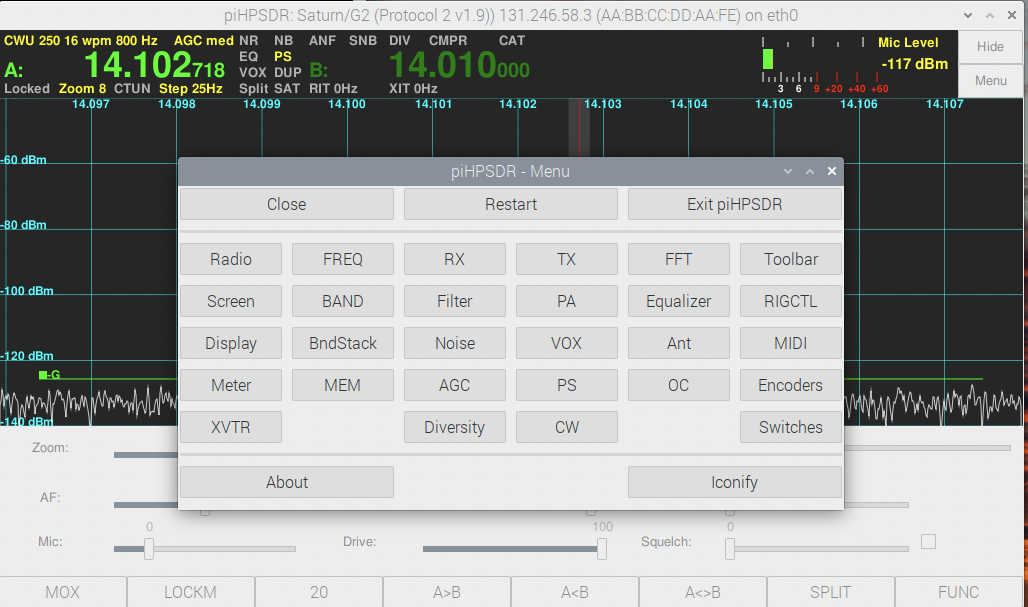
\includegraphics[width=12cm]{MainMenu.png}
\caption{The Main men, opened by the \rett{Menu} button.}
\label{fig:MainMenu}
\end{figure}

Now we have a series of chapters that discuss all the piHPDSR menus. Many menus can be
opened by a button click (or a push-botton on an external controller), e.g. hitting the
 \rett{MODE}, \rett{FILT}, or \rett{NOISE} button on the
toolbar you have seen in the last picture. You already know that the VFO and Meter
menus can be opened by clicking into the VFO or meter section at the top of the window.
When operating with a mouse, a secondary click in the RX or TX panadapter opens the
RX or TX menu. But there is one place from which \textit{all} piHPSDR menus are at hand,
and this is the "Main Menu". It can be opened by clicking into the \rett{Menu} button at the
top right corne of the piHPSDR window, the outcome is shown in Fig. \ref{fig:MainMenu}.

Some remarks have to be made about menus in general. Since piHPSDR is optimized for
working with small screens, only one menu can be open at a time. If a menu is open
and one tries to open another one, the first menu will be destroyed (closed) and the
new one will be opened. For example, if you hit the \rett{FILT} button in the toolbar
when starting from Fig. \ref{fig:MainMenu}, the main menu closes and the \bltt{Filter} menu
opens. If you try to open a menu that is already open, then the menu will be closed.
So, starting from Fig. \ref{fig:MainMenu} hitting the \rett{Menu} button again will close
the menu. Likewise, when the Filter menu has been opened, either via the Main Menu
or with the \rett{FILT} button, then hitting this button again will close the
\bltt{Filter} menu.

While the menus are looking quite diverse, some effort has been invested to keep
some things consistent throughout. For example, at the top left corner of the menu
you usually find the "Close" button which closes the menu. The close button is somewht
emphasised (slightly larger letters, and a thin border) so you will always quickly find it.
Of course, it it possible to close a menu by deleting the menu window (on RaspberryPi,
this is the small cross at the left of the title bar) but this is neither necessary nor
recommended.

There are some commands available here that do not directly affect the radio operation,
so these commands are found in the top and bottom line of the Main Menu. We first
mention the \rett{Restart} button in the middle of the top line. This restarts the
radio protocol. While not needed under normal circumstances, it my happen (especially
with beta releases of radio FPGA firmware) that the data exchange between piHPSDR and
the radio gets out-of-sync. I observed such problems with early versions of the P2
firmware for Orion2 boards and that is the reason the \rett{Restart} button is
there, since this made a quick recovery possible without loosing the QSO.
At the bottom right, there is the \rett{Iconify} button which ,,minimizes'' the
piHPSDR window. Normally, if needed, one can do so by standard methods of the
operating system in the title bar of the piHPSDR window. If piHPSDR, however,
runs in full-screen mode (this is the case on very small touch screens), then the
\rett{Iconify} button to make the piHPSDR window temporarily disappear without
breaking the connetion to the radio, do some work with the operating system, and
get the piHPSDR window back. Note in earlier versions of piHPSDR this function was
associated with the "Hide" button in the top right corner of the main window.
Then, there are two menus (\bltt{Exit} and \bltt{About}) which are described in due course and which
one can open by clicking either \rett{Exit piHPDSR} or \rett{About} in the main menu.

The other buttons, between the two horizontal separator lines, give access to piHPSDR
control and fine tuning. They are organized in six columns, namely radio related
menus (first column), VFO related menus (second column), RX and TX related menus (third
and fourth column), menus affecting both RX and TX (fifth column) and, finally,
menus for adjusting how you can control piHPSDR (sixth column), either via Toolbar,
MIDI, or GPIO encoders or switches. \textbf{,,Encoders''} are knobs which you can turn, and which
can be used to change AF volume or TX output power. \textbf{,,Switches''} are push-buttons which
can be used to trigger a function such as transmitting a carrier for tuning, toggle
between RX and TX, open a menu, and so forth.

%%%%%%%%%%%%%%%%%%%%%%%%%%%%%%%%%%%%%%%%%%%%%%%%%%%%%%%%%%%%%%%%%%%%%%%%%%%%%%%%%%%%%%%%%%%%%%%%%%%%%%%%%%%%
\section{The \texttt{Exit} Menu}

\begin{figure}[ht]
\center
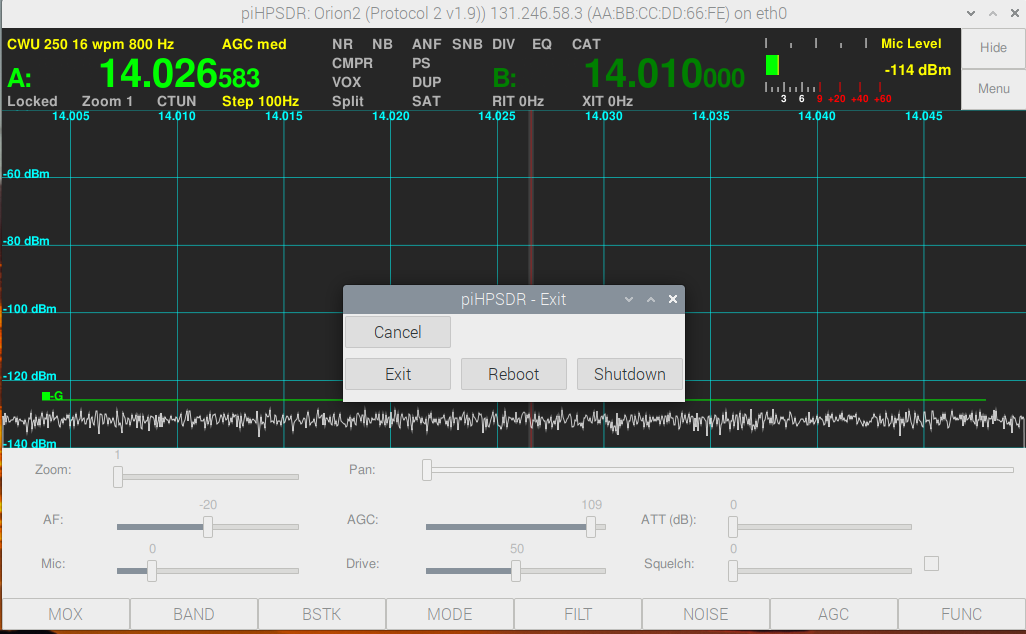
\includegraphics[width=12cm]{ExitMenu.png}
\caption{The \bltt{Exit} menu.}
\end{figure}

Via the \bltt{Exit} menu, you can leave the piHPSDR program. When leaving the program,
the radio protocol is stopped and all the settings are written to a preferences file. This
file is located in the piHPSDR directory and takes the name xx-xx-xx-xx-xx-xx.props, where
the xx encode the MAC address for the radio. So the preferences for different radios (if you
have more than one) are stored in different files. To leave the program, just click the
"Exit" button in this menu. If you decide you want to continue, you can leave the \bltt{Exit}
menu by clicking the "Cancel" button. This is the button which closes the menu and has
the same position and look as the "Close" buttons in all the other menus.

If piHPSDR runs with administrator privileges, you can even leave the program and either re-boot
or switch off the computer via the "Reboot" and "Shutdown" buttons. This makes sense for setups
where a Raspberry Pi running piHPSDR, a small SDR radio, a touch-screen and several encoders
and switches are built into a single common enclosure. On the other hand, when running
piHPSDR on desktop or laptop computers, clicking "Reboot" or "Shutdown" both leave the piHPSDR
program but no re-boot or shutdown takes place, due to missing administrator privileges.

%%%%%%%%%%%%%%%%%%%%%%%%%%%%%%%%%%%%%%%%%%%%%%%%%%%%%%%%%%%%%%%%%%%%%%%%%%%%%%%%%%%%%%%%%%%%%%%%%%%%%%%%%%%%
\clearpage
\section{The \texttt{About} Menu}

\begin{figure}[ht]
\center
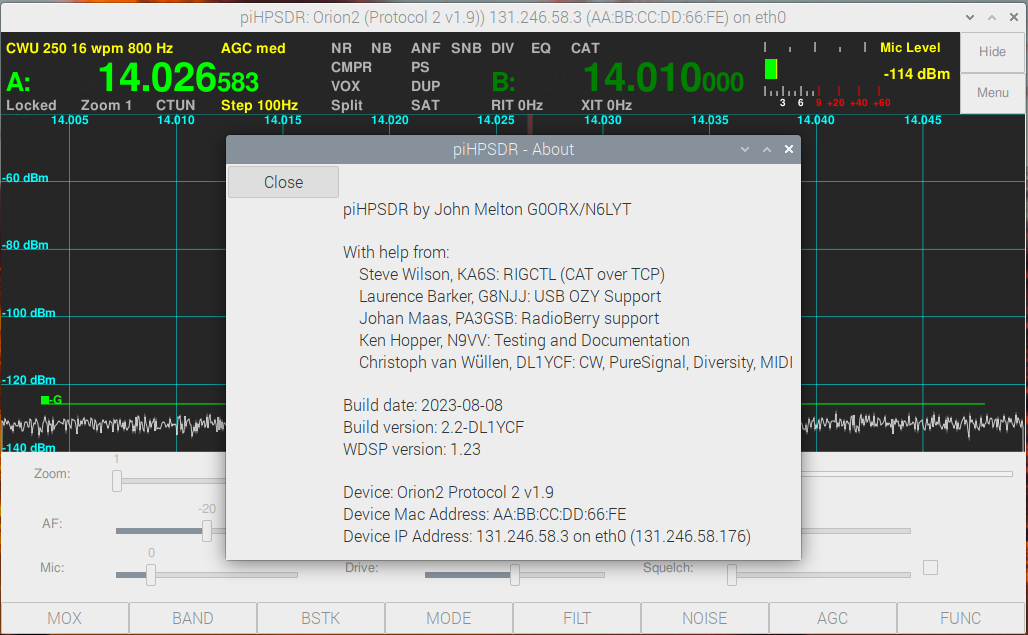
\includegraphics[width=12cm]{AboutMenu.png}
\caption{The \bltt{About} menu.}
\end{figure}

The about menu gives you some information about piHPSDR, first the original author
and an (incomplete) list
of persons who contributed to the code, and then a statement which version of piHPSDR
is working here, and when it has been compiled. Here you also find the version number of the WDSP
 library which is the ,,engine''
running under the hood, and which does nearly all of the signal processing. Finally, there is
some data on the radio, namely the device type and version numbers, and which protocol is running.
For diagnostic purposes, you also see the MAC address of the radio, its IP address and the
IP address of the computer running piHPSDR. The MAC address is of interest since the radio-specific
preferences are stored in a file whose name is derived from the radio's MAC address.

%%%%%%%%%%%%%%%%%%%%%%%%%%%%%%%%%%%%%%%%%%%%%%%%%%%%%%%%%%%%%%%%%%%%%%%%%%%%%%%%%%%%%%%%%%%%%%%%%%%%%%%%%%%%
%%%%%%%%%%%%%%%%%%%%%%%%%%%%%%%%%%%%%%%%%%%%%%%%%%%%%%%%%%%%%%%%%%%%%%%%%%%%%%%%%%%%%%%%%%%%%%%%%%%%%%%%%%%%
\chapter{The Main Menu: Radio-related menus}
\section{The \texttt{Radio} Menu}

\begin{figure}[ht]
\center
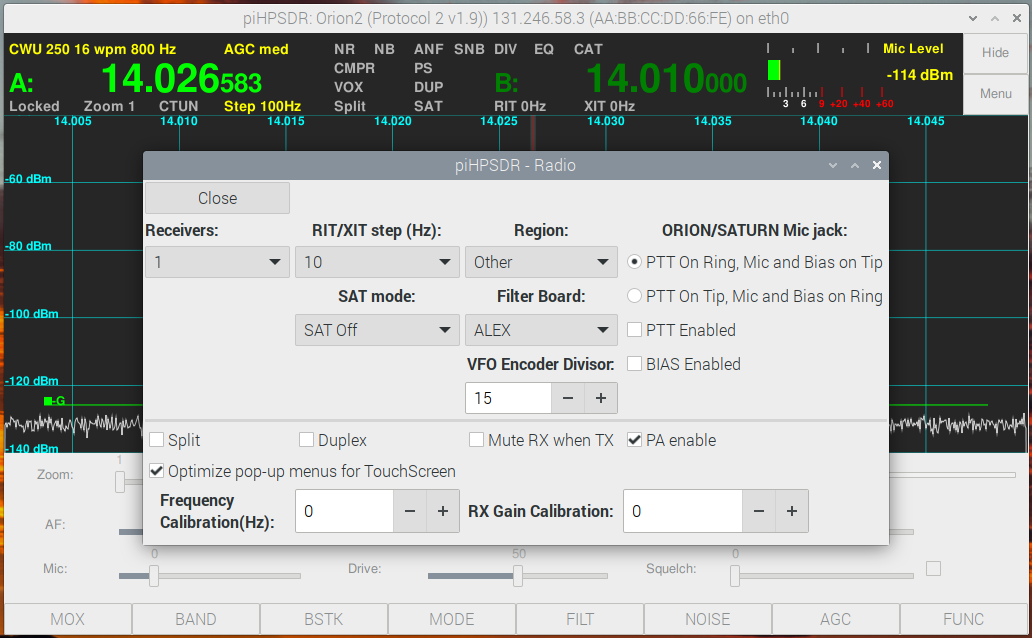
\includegraphics[width=12cm]{RadioMenu.png}
\caption{The \bltt{Radio} menu.}
\label{fig:RadioMenu}
\end{figure}


The \bltt{Radio} menu lets you make settings which affect the general setting, and the hardware of the
radio.
The following figure (Fig. \ref{fig:RadioMenu}) shows the menu as it opens on an Anan G2 radio.
Note this menu looks slightly different for different radios and protocols, this will be discussed
at the end of the section. First, we go through all the elements we see in Fig. \ref{fig:RadioMenu},
they will be colored red in the following list.

\rett{Receivers:} In the pop-down menu (GTK combo-box) below this string, you can select the number
of receivers that are running (well, you can choose between 1 and 2). When the number of receivers change,
the radio communication will shortly be stopped and then resumed, so do not be surprised if the spectrum
scope freezes for a second or so.

\rett{RIT/XIT step:} In the pop-down menu you can choose among three (1 Hz, 10 Hz, 100 Hz) step sizes
for RIT and XIT. For example, if the RIT step is 10 Hz, then you can change the RIT offset in steps of
10 Hz with the RIT+ or RIT- buttons in the toolbar or on the GPIO/MIDI controller.

\rett{Region:} Although not obvious, this selects settings for the 60m band. Possible choices are "Other",
 "UK" and "WRC15". The \texttt{Other} and \texttt{UK} choices implement the channel structure of the 60m
 band according to the regulations valid in the USA and Great Britain. "WRC15" gives you a small (15 kHz
 wide) 60m band according to the WRC15 (World Radio Conference 2015) document, which is now implemented in
 many countries.

\rett{Orion/Saturn Mic jack:} This part of the menu is not shown for pre-Orion boards.
The Orion, Orion2, and Saturn boards can switch the connections
 of the TRS microphone jack in software (hardware jumpers had to be used previously).
While the ring of the TRS plug is always connected to ground, the microphone and PTT connections are on the
ring an tip and you can choose which one is on the ring and which one on the tip. You can then separately
enable the PTT function of the jack, and select whether a bias (DC offset) is applied to the mic connetion
(this is necessary for condensor microphones and detrimental if a dynamic mirophone is connected without
a blocking capacitor).

\rett{Mic Input:} This is only shown for Saturn boards. These radios have two jacks for connecting a
microphone, either a 3.5mm TRS jack in the front panel, or an XLR connection in the back panel. The pop-down
menu lets you choose between these two options.

\rett{SAT mode:} Here you can choose between \texttt{SAT off}, \texttt{SAT}, and \texttt{RSAT}. In SAT mode,
frequency moves applied to one of the two VFOs are applied to the other VFO as well. This is convenient
for cross-band operation over satellites with (normal) linear transponders. In RSAT mode, frequency
moves applied to one of the two VFOs are applied to the other with the sign inversed, that is, if
for example you move the frequency of VFO A up by 3 kHz, the frequency of VFO B moves down by the same
amount. This is convenient for cross-band operation over satellites with inverted transponders. Inverted
transponders are sometimes find in low and fast moving satellites because this leads to some Doppler
 correction.

\rett{Filter board:} Normally SDRs have some sort of built-in PA with a filter board. Filters in the TX path
between the PA and the antenna are always required, and filters in the RX path provide some protection
against ADC overloads from strong out-of-band signals. Here you can choose between \texttt{NONE},
\texttt{ALEX},
\texttt{APOLLO}, \texttt{CHARLY25}, and \texttt{N2ADR}. Choose \texttt{NONE} if none of the other cases
apply, and hope your radio does things right automatically. \texttt{ALEX} is the most frequent choice
and applies to the largest part of current HPSDR radios. \texttt{APOLLO} is an early design of a
PA/filter combination for Hermes boards, choose this if you have one. \texttt{CHARLY25} is a filter board
used in some RedPitaya based radios (STEMlab and HAMlab). If you choose this, the Attenuator slider will
disappear from the Slider area (because this design does not have a step attenuator), instead, you get
a combined Attenuator/Preamp check-box which lets you choose between zero, preamp values of 18 and 36 dB,
and attenuation values of 12, 24, and 36 dB. \texttt{N2ADR}, finally, is the filter board usually used
in combination with a HermesLite-II radio. It is controlled by the OC (open collector) bits in the HPSDR
protocoll. This means if you use \texttt{N2ADR}, this will override your OC settings upon program startup.
It is possible to change the OC settings in the \bltt{OC} menu, and these settings are saved with the
preferences. Upon next program start, however, these preferences will again be overwritten as long
as the \texttt{N2ADR} filter board is chosen.

\rett{VFO Encoder Divisor:} This option is normally only used for GPIO controllers. Often, the
encoders of the main VFO dial generate too many ticks per revolution, such that it is difficult
to fine tune on a signal. If the VFO Encoder Divisor, as shown in the example, has a value of
15, only every 15$^\textrm{th}$ tick will we processed. The Divisor is also effective if you
control piHPSDR with an ANDROMEDA console. So, if the frequency moves too fast if you turn
the VFO knob, you have to increase the Divisor, and if it moves too slowly, decrease it.

\rett{Split} Use this checkbox to enable/disable Split mode. In Split mode, the frequency of
the non-active receiver (when using two receivers) or the frequency of VFO-B (when using one
receiver) controls the TX frequency. In normal (non-Split) mode, it is the frequency of
the active receiver (2 RX) or the frequency of VFO-A (1 RX) that matters.

\rett{Duplex} Use this checkbox to enable/disable Duplex mode. In Duplex mode, the receiver(s)
continue working during TX. In normal setup, this is detrimental since the very strong
signal that originates from the crosstalk at the T/R relay will lead to AGC pumping,
making your receiver(s) essentially deaf for a short period after TX/RX switching.
However, when using different and well-decoupled antennas for RX and TX (this is typical
for some satellite operations), Duplex mode gives you important information, as you can
see your own downlink signal. In contrast to what is often stated, Duplex mode does not
affect the data stream between the computer and the radio, it \textit{only} determines
whether the receivers (within the WDSP library) are shut down during transmit or not.

\rett{Mute RX when TX} This option mutes the RX audio while transmitting. It is important
to note that the RX continue to work, so you can see the signals on the RX panel, the
S-meter works, etc. This option is largely equivalent to moving the AF slider to the
minimum position while transmitting.

\rett{PA enable} This enables/disables the PA in the radio. In addition to this global
flag, there is a per-band PA enable option for the transverter bands (see the \bltt{XVTR}
menu).

Note that the last four options (\rett{Split}, \rett{Duplex}, \rett{Mute RX when TX},
and \rett{PA enable} are not shown for RX-only radios.

\rett{Optimize for TouchScreen} The normal procedure to make a selection from a
pop-down menu (such as the \rett{Receivers:} button on this screen) is to click
(and hold) it with a mouse, then drag the mouse to your choice, and then the selection
is made by releasing the mouse button. This is very difficult to achieve on a touch
screen. Therefore, if \rett{Optimize for TouchScreen} checkbox is checked, the pop-down
menus are modified as follows: You click and release on the menu button, then it pops
down and stays open. Then you make your selection by a second click/release sequence
on your choice. While this is (only a little bit) more involved than the normal procedure
when using a mouse, it is a great helper when using a touch screen. Therefore this
option is set by default, but you can uncheck it here if you prefer normal
mouse operation. Note that this option becomes effective when the next menu is opened.

\rett{Frequency Calibration} Here you can set a frequency offset (in Hz). This offset
will be added to all frequencies sent to the radio. This means that if you discover that
a reference signal occurs in your RX panel at 10001 kHz where it should occur at 10000
kHz, you have to set the calibration value to -1000. Note it is an absolute value,
which will we applied to all frequences.

\rett{RX Gain Calibration} Here you can calibrate your RF front end. To this end, you
need a highly accurate signal source of, say, -73 dBm. Connect this source to your
radio and tune on the signal. If the signal appears at, say, -70 dBm, decrease the
calibration value. At -3 dBm, your S-meter should then state the correct signal
strength. The value is the  amplification/attenuation of  a virtual device you
would need in your RF front end. Therefore, you need a negative value (attenuation)
if the signal shown is too strong. For normal HPSDR radios, the default value is
 zero. For the HermesLite-II and other radios using the AD9866 chip, the default
 value is 14.

 There are some further check boxes in the \bltt{Radio} menu that you cannot see
 in Fig. \ref{fig:RadioMenu}, since they only appear for specific radio hardware.
 They appear to the right of the touch screen optimization check box
 and will be listed here.

 \rett{HL2 audio codec} This box only appears if the radio is a HermesLite-II (HL2). Some
 of these radios are equipped with an audio codec and a modified firmware. The
 audio codec must be enabled by setting a specific bit in the HL2 protocol,
 and this check box enables/disables this bit. Furthermore, if this check box
 is enabled, RX audio data is sent to the HL2.

 \rett{Anan-10E/100B} This box only appears for Hermes boards. While the Anan-10E and
 the Anan-100B identify themselves as Hermes boards, they have a FPGA with limited
 resources and this affects the allocation of PureSignal feedback channels. To make
 PureSignal work on these machines, you have to check this box in the \bltt{Radio} menu.

 \rett{Swap IQ} This box only appears for radios connected via the SoapySDR library. If checked
 the I and Q samples are exchanged, both in the receivers and in the transmitter. An indication
 that this is necessary is if you see signals with a frequency above your dial frequency in
 the left half of the RX panel, or if you have to go to LSB to receive USB signals. If you
 observe this behaviour, check this box.

 \rett{Hardware AGC} This box only appears for radios connected via the SoapySDR library.
 If checked, automatic gain control (AGC) that is implemented in hardware in the radio is enabled.

 \textbf{ATLAS bus options.} For legacy ATLAS bus radios, a number of additional settings have to be
 made. Therefore, the area where we have seen the Orion microphone options now contains ATLAS bus
 settings, as shown in Fig. \ref{fig:RadioMenuMetis}. You will see this only if the radio identifies
 itself as a METIS board.

\begin{figure}[ht]
\center
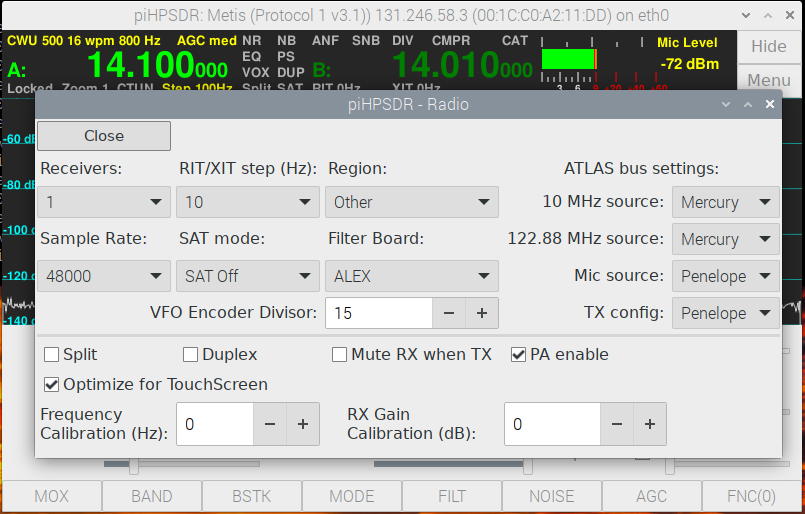
\includegraphics[width=12cm]{RadioMenuMetis.png}
\caption{The \bltt{Radio} menu for a legacy HPSDR board.}
\label{fig:RadioMenuMetis}
\end{figure}

The first difference you notice is that at the left edge of the menu, in the middle,
there is a new \rett{Sample Rate:} pop-down menu. This has nothing to do with the
ATLAS bus, this occurs if the radio is connected via P1, as it is often the case for
legacy radios. In P1, all receivers share the sample rate, therefore it is set in the
\bltt{Radio} menu. The same applies for SoapySDR radios. In P2 on the other hand, each
of the two receivers can have its own sample rate, therefore the sample rate is specified
in the \bltt{RX} menu. The ATLAS bus settings are at the right edge of the menu (see Fig.
\ref{fig:RadioMenuMetis}. The ATLAS bus has separate receiver and transmitter plug-in boards.
To build a radio, they must be synchronized somehow, and therefore their clocks cannot run
independently, but there must be a master clock.

\rett{10 Mhz source:} This selects the 10 Mhz master clock, which can be either \texttt{ATLAS}
(the bus itself is the source), \texttt{Penelope} (the transmitter board is the source),
or \texttt{Mercury} (the receiver board is the source).

\rett{122.88 MHz source:} This selects the 122.88 Mhz master clock, which can be either
\texttt{Penelope} or \texttt{Mercury}.

\rett{Mic source:} This selects where the microphone samples that are sent to the computer
originate, that is, where your microphone has to be connected. The default is
\texttt{Penelope}, this means the microphone is connected to the transmitter board. The
other choice is \texttt{Janus}. The \texttt{Janus} board is simply an ADC/DAC board (not
a radio) and used in some very early setups.

\rett{TX config:} This indicates which transmitter board is present on the bus. It can
be \texttt{No TX}, if this is a receive-only radio, \texttt{Penelope} or \texttt{Pennylane}.
The \texttt{Pennylane} is a later version of the Penelope transmitter board, the essential
difference is that it can control the output signal level. In the Penelope case,
piHPSDR will scale the IQ samples to provide TX drive control.

\rett{Janus Only} This box is for ATLAS systems that only have an OZY and a Janus board,
and will only appear for OZY (USB-connected) boards. While this hardware is not a radio,
external hardware such as the SDR-1000 can be connected to the Janus interface. If this
option is checked, piHPSDR assumes that the radio is controlled outside piHPSDR, and
will thus only process the data stream but not try to send any commands to the radio.

Note that I have no access to such legacy radios, so the piHPSDR code to handle these radios
is partly built on speculation (that is, studying the specs) and exchanging e-mails with
people who still run such hardware. If you meet any inconsistencies, please contact
the author.

%%%%%%%%%%%%%%%%%%%%%%%%%%%%%%%%%%%%%%%%%%%%%%%%%%%%%%%%%%%%%%%%%%%%%%%%%%%%%%%%%%%%%%%%%%%%%%%%%%%%%%%%%%%%
\section{The \texttt{Screen} Menu}

The \bltt{Screen} menu lets you dynamically change the size of the piHPSDR main
window, and choose between different VFO bar layouts. The possibility to adjust
the screen size has been the most frequent feature request in the last years,
so I finally decided to implement it. The menu is opened
via the main menu and the \bltt{Screen} button and is shown in Fig. \ref{fig:ScreenMenu}.

\begin{figure}[ht]
\center
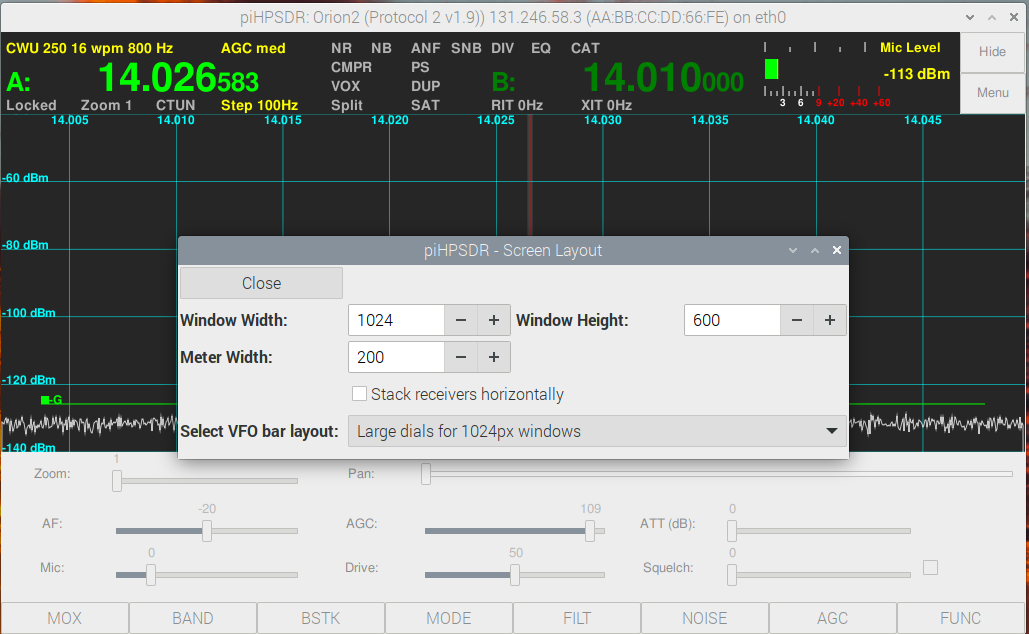
\includegraphics[width=12cm]{ScreenMenu.png}
\caption{The \bltt{Screen} menu.}
\label{fig:ScreenMenu}
\end{figure}

The window width and height can be chosen with the spin buttons shown. The minimum
values for width and height are 640 and 400, the maximum values are determined by
the resolution of the monitor. If more than one monitor is attached, the dimension
of the monitor on which the initial piHPSDR window was opened determines
the maximum width and height. Changes made in the spin buttons become effective
immediately. If piHPSDR is in full screen mode (see below), you can change the
values of the window width and height, but they do not become effective until
you leave the full screen mode.

\begin{figure}[ht!]
\center
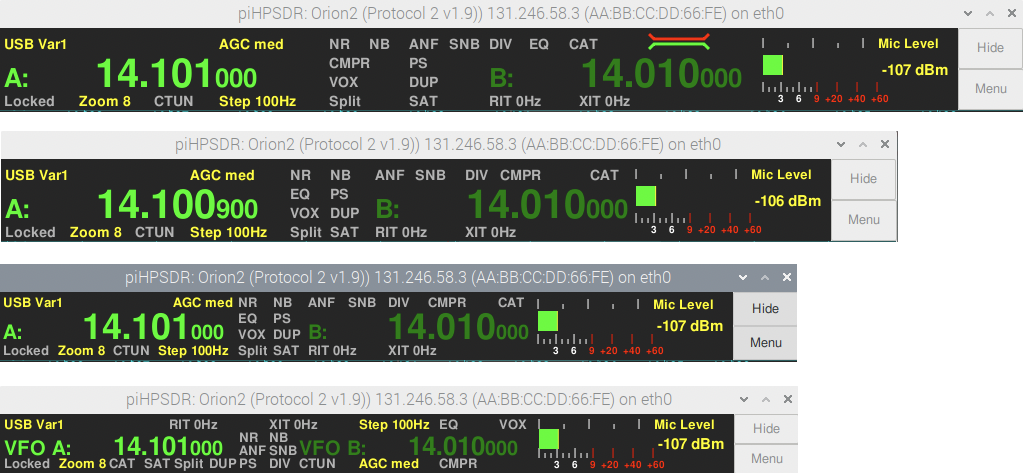
\includegraphics[width=12cm]{VFObarChoice.png}
\caption{Four choices for the VFO bar built into piHPSDR.}
\label{fig:VFObarChoice}
\end{figure}

If the window width is decreased such that the VFO bar chosen does no longer fit,
the first one in the list that does fit is automatically selected, and the
current choice shown in the
 pop-down menu \rett{Select VFO bar layout} is updated. This menu lets you choose
 the layout of the VFO
bar. In Fig. \ref{fig:VFObarChoice} the pre-defined layouts are shown.



These layouts require a screen size of 1010, 895, 795, and 635 pixels (from top to
bottom).
The VFO bar has been described in detail in chapter
\ref{sec:VFObar}. If you choose a VFO bar layout that is wider than the current
window width allows, the window width is automatically adjusted (increased). On the
other hand, choosing a VFO bar layout that is smaller than before does not affect
the screen dimensions.

\begin{figure}[ht!]
\center
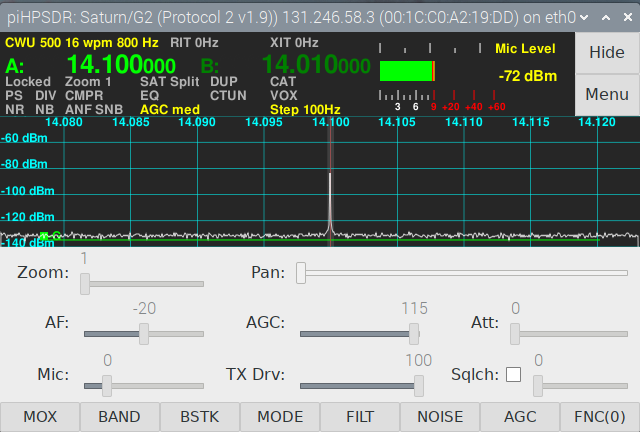
\includegraphics[width=9cm]{640x400.png}
\caption{piHPSDR running in a 640 x 400 window.}
\label{fig:640x400}
\end{figure}

Fig. \ref{fig:640x400} shows, as an example, piHPSDR running in a window as small
as 640*400 pixels. It is admitted that this looks rather squeezed, and this
will only be useful if a single receiver is run with no waterfall. However, for
portable operations such small windows are often desired,
if piHPSDR is to be run alongside with a logbook and/or digimode program on a small laptop.
Note that the piHPSDR menus are designed to fit on a window 800*480 pixels large, so
it is not recommended to run piHPSDR on a \textit{screen} that small. On the other hand,
if piHPSDR is run on a laptop in a small 640*400 window, then menus may be larger than
that but still fit well on the screen (thus hiding, momentarily, the window of,
say, your logbook program) and are perfectly usable.

\rett{Stack receivers horizontally}. If checked, this puts the panels
of the two receivers (if two receivers are used) side-by-side instead of on top
of each other.

\rett{Full Screen Mode}. If you check this option, piHPSDR goes to full screen mode.
In this mode, the window width and height is ignore, instead, piHPSDR occupies
the whole area of the screen. In a multi-monitor setup, the area of the monitor
on which the piHPSDR window was opened upon program start is filled.
If you leave full screen mode, the size of the piHPSDR window is again
determined by the width and height chosen above.

%%%%%%%%%%%%%%%%%%%%%%%%%%%%%%%%%%%%%%%%%%%%%%%%%%%%%%%%%%%%%%%%%%%%%%%%%%%%%%%%%%%%%%%%%%%%%%%%%%%%%%%%%%%%
\section{The \texttt{Display} Menu}

The \bltt{Display} menu is used to customize the overall layout of the piHPSDR
window and the RX panadapters. Adjustments
for the TX panadapter must be done in the \bltt{TX} menu. The menu is shown
in Fig. \ref{fig:DisplayMenu}.

\begin{figure}[ht]
\center
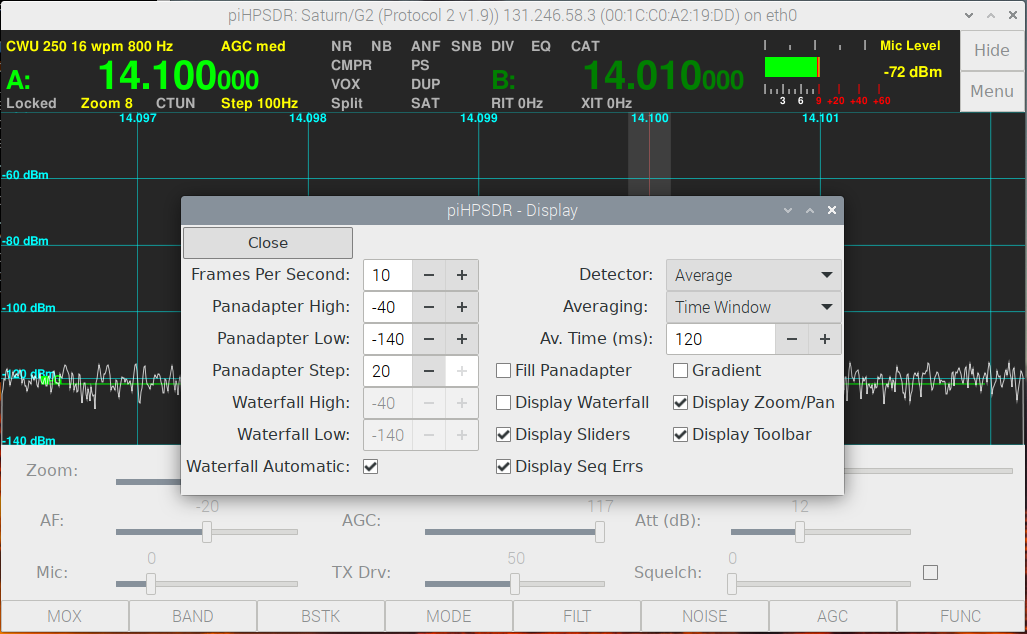
\includegraphics[width=12cm]{DisplayMenu.png}
\caption{The \bltt{Display} menu.}
\label{fig:DisplayMenu}
\end{figure}

\rett{Frames Per Second:} This adjust how often the RX and TX (!) displays are re-drawn.
10 frames per second (the default) is a good value.

\rett{Panadapter High:} This value is the dBm value of the RX signal strength at the
top of the RX spectrum scope. A value of -40 dBm corresponds to S9 + 33 dB for HF
signals.

\rett{Panadapter Low:} This value is the dBm value of the RX signal strength at the
bottom of the RX spectrum scope. A value of -140 dBm is usually low enough such that
the noise floor is still on display.

\rett{Panadapter Step:} This value is the spacing of the horizontal lines on
the spectrum scope. Lines are drawn at dBm values that are multiples of the step
size.

\rett{Waterfall High:} This is the RX dBm value that will lead to the brightest
color (yellow) in the waterfall.

\rett{Waterfall Low:} This is the RX dBm value below which the waterfall will be black.

\rett{Waterfall Automatic:} If this box is checked, the \rett{Waterfall High} and
\rett{Waterfall Low} controls are inactive and the values are not used. Instead,
the lowest and highest signal strength in the RX spectrum are automaticall determined
in each update of the waterfall, and these min/max values
 are then used instead of the waterfall High/Low control values to determine which
 colour belongs to which signal strength.

\rett{Detector:} Here one can choose between Peak, Rosenfell, Average and Sample. The
Rosenfell detector is probably closest to what one knows from a spectrum analyzer.
The Average detector is usually preferred since it is less ,,nervous''.

\rett{Averaging:} Here the possible choices are None, Recursive, Time Window and
Log Recursive. For the details, see the WDSP manual.

\rett{Av. Time (ms):} If averaging is used for the spectrum scope, the time
constant involved in averaging can be set here.

\rett{Fill Panadapter} This is used to enable/disable the ,,Filling'' option
for the RX and TX spectrum scopes (see chapter \ref{sec:FillingGradient}).

\rett{Gradient} This is used to enable/disable the ,,Gradient'' option
(color coding) for the RX spectrum scope (see chapter \ref{sec:FillingGradient}).
 Note color coding is not available for the TX panel.

 \rett{Display Waterfall} This option enables/disables the waterfall display
 of the RX panels. Note the spectrum scope is always shown (you cannot have the
 waterfall alone).

 \rett{Display Zoom/Pan} This option can be used to show/hide the Zoom and
 Pan slider below the RX or TX panel. If you do not use Zoom, or control
 Zoom via an external GPIO or MIDI controller, this can be used to save
 some vertical space.

 \rett{Display Sliders} This option can be used to show/hide the slider area
 (that is where the AF or TX Drive slider resides).
 Hiding them makes little sense unless you
 have a GPIO or MIDI controller. For temporarily gaining vertical space,
 use the \rett{Hide} button at the top right of the main window.

 \rett{Display Toolbar} This option can be used to show/hide the toolbar. This
 only makes sense of using an external GPIO or MIDI controller. Note that
 when using the piHPSDR Controller1, the toolbar should remain on display since
 this then serves as an indication which function is associtated with each of
 the 8 push buttone immediately below the screen.

\rett{Display Seq Errs} All data packets from the radio to the PC contain
a sequence number that is increased  for each packet sent. piHPSDR
checks for each incoming data packet whether the sequence number is
exactly larger by 1 than the number of the previous packet. If this is not
the case, this is a \textit{sequence error}. Sequence errors may be caused
by loosing packets on the way from the radio to the computer, or
(this is what is usually the reason) packets lost within the computer due
to the computer being busy with something else (e.g. writing to disk).
 If the \rett{Display Seq Errs} is checked, a red
,,Sequence error'' message appears in the RX panel for two seconds.
Sequence errors during RX often cause cracks in the RX audio. Unless this
happens regularly, it is no reason to worry.


%%%%%%%%%%%%%%%%%%%%%%%%%%%%%%%%%%%%%%%%%%%%%%%%%%%%%%%%%%%%%%%%%%%%%%%%%%%%%%%%%%%%%%%%%%%%%%%%%%%%%%%%%%%%
\section{The \texttt{Meter} menu}

\begin{figure}[ht]
\center
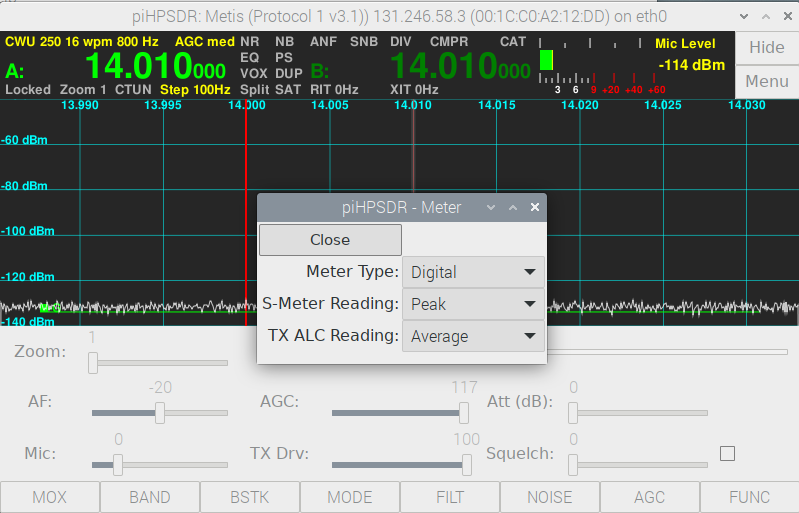
\includegraphics[width=12cm]{MeterMenu.png}
\caption{The \bltt{Meter} menu.}
\label{fig:Meter}
\end{figure}

The \bltt{Meter} can either be opened simply by clicking in the meter
area, or through the main menu. Only few choices can be made here.

\rett{Meter Type:} Here you can select between a digital and an analog
meter. The four different designs (either analog or digital, and during
RX or TX) have already been shown in Sec. \ref{sec:MeterSection}.

In both cases, there is a choice between Peak and Average reading, which
refers to peak envelope power and average power. Here averaging is done
over relatively short times. For a two-tone signal for example, the peak
reading is 3 dB above the average reading.

\rett{S-Meter Reading:} Here you can choose whether the S-meter reports
a Peak or an Average value (default is Average).
Note, however, that in order to make the
display less ,,nervous'' a moving average with a rather long time constant
(about 0.5 sec) has been implemented on top of both the Peak and Average
S-meter readings.


\rett{TX ALC reading:} Here, the possible values are Peak, Average, and
ALC gain. For a two-tone signal with maximum audio amplitude the Average
ALC value is -3.0 dB, while the Peak value is 0.0 dB. Therefore I personally
prefer the Peak value here and made it the default in piHPSDR:
 if the value is less than zero, one can and should
increase either the amplitude of the incoming audio signal (e.g. boost the
microphone preamp) or move the Mic gain slider to the right. The reason is,
that PureSignal only works if the TX audio input has maximum amplitude,
so you can put the drive slider to zero, then put the radio into TX mode,
whistle into the microphone and slowly increase the Mic gain until the
ALC value shown is only slightly less than zero.

For RX-only radios, the TX ALC setting will not be shown in the menu.

%%%%%%%%%%%%%%%%%%%%%%%%%%%%%%%%%%%%%%%%%%%%%%%%%%%%%%%%%%%%%%%%%%%%%%%%%%%%%%%%%%%%%%%%%%%%%%%%%%%%%%%%%%%%
\section{The \texttt{XVTR} (Transverter) Menu}

The \bltt{XVTR} menu lets you define additional bands
that you can work on using transverters. The bands
should normally be beyond the standard frequency range of
the radio, otherwise the calculation of a band from
a given frequency will sometimes not work. To give an example,
suppose you have a transverter which you can drive with frequencies
between 28 and 30 MHz and which will convert them to the frequency
range 144 to 146 MHz, and which will receive frequencies in that
range and mix them down to the 10m band. The data you have to enter
in the \bltt{XVTR} menu (use the first free entry) are as follows:
\begin{figure}[ht]
\center
\includegraphics[width=12cm]{XVTRMenu.png}
\caption{The \bltt{XVTR} (transverter) menu.}
\label{fig:XVTRMenu}
\end{figure}



\rett{Title} In this column, enter a name for your band. You can choose
whatever name you want, this is the one that will be displayed in the
\bltt{Band} menu. In the present example, use "144" or "144 MHz" or "2m".

\rett{Min Freq} Enter the lowest frequency of the transverter band in MHz,
in the present case, 144.

\rett{Max Freq} Enter the highest frequency of the transverter band in MHz,
in the present case, 146.

\rett{LO Freq} This is the frequency offset (in MHz) between the radio frequency and
the operating frequency. In this case, use 116. From this offset, radio frequencies
between 28 and 30 MHz will be used for operating frequencies between 144 and 146 MHz.

\rett{LO Err} This entry can be used for a fine calibration of the frequency. The value
(in Hz) is added to the local oscillator (LO) freq in MHz.

\rett{Disable PA} This checkbox indicates that the PA of the radio should be disabled
when using the transverter band. This implies that the radio has some sort of
low-power output that is used to drive the transverter.

\begin{figure}[h!]
\center
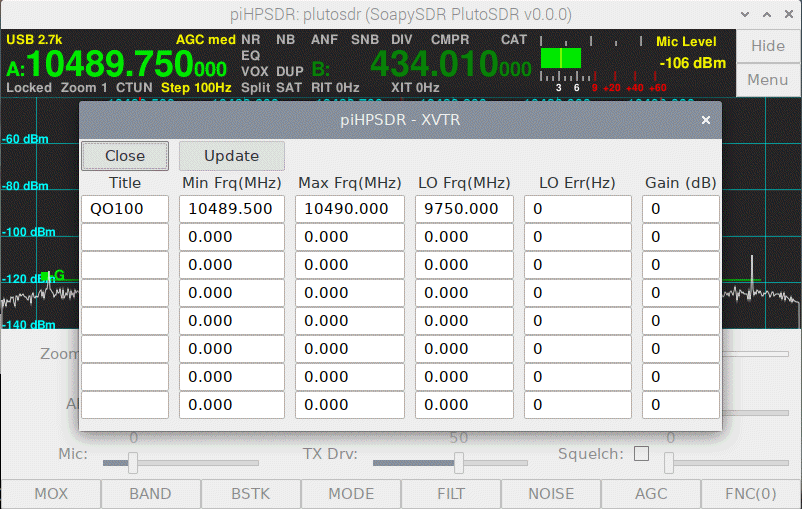
\includegraphics[width=12cm]{QO100-XVTR.png}
\caption{\bltt{XVTR} setup for QO-100 operation.}
\label{fig:QO100-XVTR}
\end{figure}

To give an example of how to setup transverter operation, a sample setup for QO-100 operation
with an Adalm Pluto is given.
The Pluto is
operated via the SoapySDR interface. For receiving in the 10 GHz band, one uses a so-called
LNB (low noise block) in the focus of the parabol antenna which converts the 10 GHz signal down
to about 740 MHz. The setup for defining the "QO100" transverter band is shown in Fig.
\ref{fig:QO100-XVTR}.

The LO (local oscillator) frequency is always chosen such that it is below the RX frequency,
and the difference between the RX frequency and the LO frequency is the frequency the radio
is operating on. The name (here: QO100) can be chosen as one likes, but it cannot be left
empty. Once the transverter band has been defined, it shows up in the \bltt{BAND} menu
(see Chapter \ref{sec:bandmenu}), as shown in Fig. \ref{fig:QO100-BandMenu}.

\begin{figure}[ht]
\center
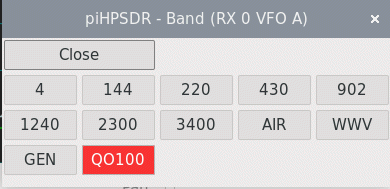
\includegraphics[width=6cm]{QO100-BandMenu.png}
\caption{The \bltt{Band} menu after defining the QO100 band.}
\label{fig:QO100-BandMenu}
\end{figure}

To make QO-100 Operation easy, the working frequencies, the CTUN mode etc. should be
stored in the first bandstack entry of the QO100 and the 13 cm band. To this end,
click on the QO100 in the band menu (Fig. \ref{fig:QO100-BandMenu} and adjust the VFO-A
frequency until the display reads 10489.500 MHz. Now swap VFO-A and VFO-B (\bltt{A<>B} command)
and enter 2400 MHz into VFO-A using the \bltt{VFO} menu (Chapter \ref{sec:vfomenu}). and
swap the VFOs again. SAT mode will now ensure the 10.489 GHz Receive
 Frequencies and the 2.4GHz Transmit frequencies track correctly when changes are made
 to the Receive frequency. PiHPSDR will now remember these settings when you select
 the bands. The complicated swapping was necessary since band stack entries will
 only be stored from VFO-A.

Fig. \ref{fig:QO100-Waterfall} gives an impression of how this actually works. Note that the
default setup
is working Split, Duplex and SAT. Split mode implies that VFO-B is used for transmitting.
Duplex mode implies that the receiver continues to work while transmitting so you can watch
and hear your own signal.
The TX spectrum scope then appears during transmitting in a small separate window.
\begin{figure}[ht]
\center
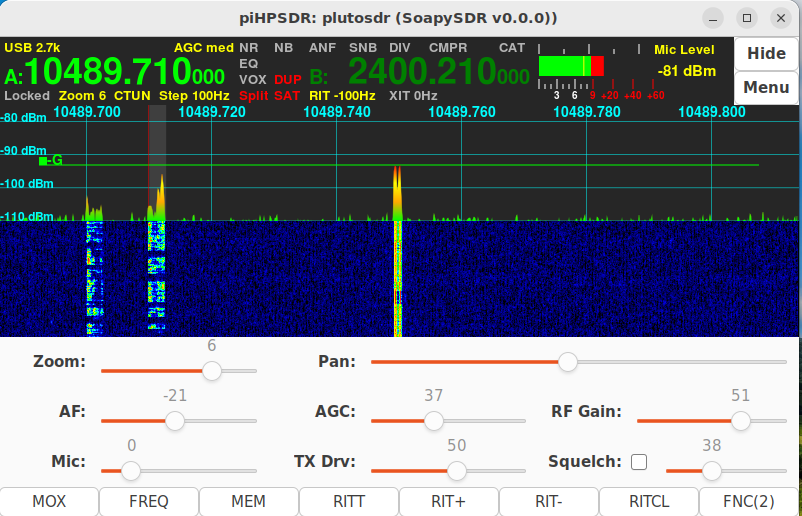
\includegraphics[width=12cm]{QO100-Waterfall.png}
\caption{Working QO100 with piHPSDR and the Pluto.}
\label{fig:QO100-Waterfall}
\end{figure}
%%%%%%%%%%%%%%%%%%%%%%%%%%%%%%%%%%%%%%%%%%%%%%%%%%%%%%%%%%%%%%%%%%%%%%%%%%%%%%%%%%%%%%%%%%%%%%%%%%%%%%%%%%%%
%%%%%%%%%%%%%%%%%%%%%%%%%%%%%%%%%%%%%%%%%%%%%%%%%%%%%%%%%%%%%%%%%%%%%%%%%%%%%%%%%%%%%%%%%%%%%%%%%%%%%%%%%%%%
\chapter{The Main Menu: VFO-related menus}

In this chapter we discuss the menus from the second column
of the main menu. These are all VFO-related menus.


\section{The \texttt{VFO}  menu}
\label{sec:vfomenu}
\begin{figure}[ht]
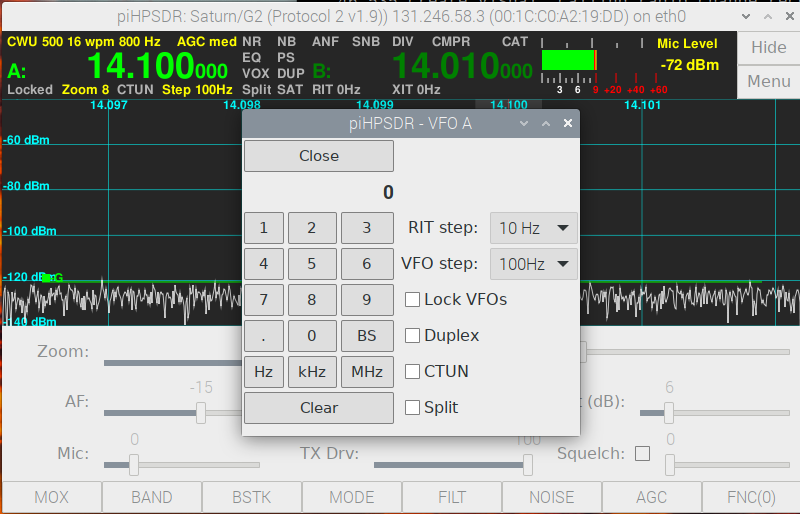
\includegraphics[width=12cm]{VFOmenu.png}
\caption{The \bltt{VFO} menu.}
\label{fig:VFOmenu}
\end{figure}

The \bltt{VFO} menu can be used for direct frequency entry and to
enable/disable some frequently used options. If the menu is opened,
it refers either to VFO-A or VFO-B. If opened via the main menu,
it automatically refers to the VFO controlling the active receiver.
The easiest (and therefore recommended) way to open the \bltt{VFO}
menu is just to make a mouse click (or a touch screen press) into the
VFO bar. If clicked in the left half of the VFO bar, the menu is opened
for VFO-A and if clicked in the right half, it is opened for VFO-B.
The \bltt{VFO} menu is shown in Fig. \ref{fig:VFOmenu}.


The ,,keypad'' is used for direct frequency entry. You can enter
digits and a decimal point. While entering a number the string
entered so far is not only shown in the upper part of the
\bltt{VFO} menu, but also (in yellow digits) in the VFO bar.
The other buttons of the ,,keypad'' have a special meaning:



\rett{BS} Backspace. This cancels the last entered character
(digit or decimal point).

\rett{Hz} This enters the frequency ,,as is''.

\rett{kHz} This multiplies the frequency just entered with 1000 and
enters it. This means, the number entered is interpreted as a
frequency in kHz.

\rett{MHz} The string typed in so far is interpreted as a frequency in MHz
and this frequency is transferred to the VFO.

\rett{Clear} The string typed in so far is deleted, the VFO frequency is not
updated.

The commands entered by clicking the buttons of the keypad in the VFO menu
can also be entered by push-buttons from a GPIO or MIDI controller, see
the NumPad commands in Appendix A.

In addition to frequency entry, the VFO menu offers a convenient way of changing
some piHPDSR settings, simply because the VFO menu can be opened by a simple
mouse click into the VFO bar.

\rett{Rit Step:} In this pop-down menu, the RIT/XIT step size can be chosen
 (1/10/100 Hz).

\rett{VFO Step:} In this pop-down menu, the VFO step size can be chosen. The VFO step
sizes range from 1 Hz to 1 MHz.

\rett{Lock VFOs} With this check box enabled, VFO frequencies cannot be changed by
turning a VFO dial (GPIO or MIDI controller), or by clicking/dragging in the RX panel.
Band changes (via the \bltt{Band} menu) and other VFO related functions still work.

\rett{Duplex} and \rett{Split}. With these check boxes, you can put the radio
in Duplex or Split mode, see the \bltt{Radio} menu.

\rett{CTUN}. With this check-box, you can put the VFO this menu is referring to into
CTUN mode. In CTUN mode, the spectrum scope does not move when changing the frequency,
rather, the RX ,,window'' moves. CTUN mode does not affect TX operation.

%%%%%%%%%%%%%%%%%%%%%%%%%%%%%%%%%%%%%%%%%%%%%%%%%%%%%%%%%%%%%%%%%%%%%%%%%%%%%%%%%%%%%%%%%%%%%%%%%%%%%%%%%%%%
\section{The \texttt{Band} menu}
\label{sec:bandmenu}
The \bltt{Band} menu lets you change the band of the active receiver. It is shown
in Fig. \ref{fig:BandMenu}. When the menu opens, the button of the current band
is highlighted.

\begin{figure}[ht]
\center
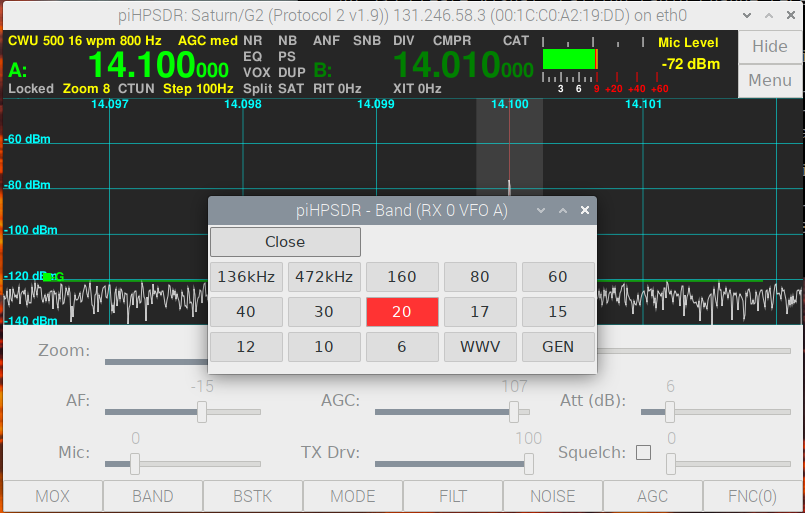
\includegraphics[width=12cm]{BandMenu.png}
\caption{The \bltt{Band} menu.}
\label{fig:BandMenu}
\end{figure}

Pressing a button corresponding to another band, two things happen: first, if the
active receiver is controlled by VFO-A, the current frequency is stored in the current
bandstack (which is thus updated). Then, the new band is chosen, the frequency and mode
are from the active bandstack entry of the new band. This means that if you switch
to another band and shortly thereafter switch back to the original band, the
frequency and mode is restored to what you had before.

If you hit the highlighted button, you will not change the band (since you hit the
button of the current band) but instead will cycle through the band stack of that band
(see the \bltt{BndStack} menu).


Note that the band menu may look different from the one shown here: there are many bands
(24 bands plus up to 8 transverter bands) defined in piHPSDR. However, the bands that
are outside of the radio's frequency limits are not shown. For example, a radio
whose maximum frequency is 30 Mhz will not show the 6m band. The \rett{GEN} (General)
band encompasses the whole frequency range of the radio. If you set the frequency
(e.g. via the \bltt{VFO} menu) to a frequency outside of any of the other bands, you
will end up in the General band. If you have defined transverter bands (see the
\bltt{XVTR} menu) they will be shown, with the title you have chosen, in the
\bltt{Band} menu.

%%%%%%%%%%%%%%%%%%%%%%%%%%%%%%%%%%%%%%%%%%%%%%%%%%%%%%%%%%%%%%%%%%%%%%%%%%%%%%%%%%%%%%%%%%%%%%%%%%%%%%%%%%%%
\section{The  \texttt{BndStack} (Bandstack) menu}

\begin{figure}[ht!]
\center
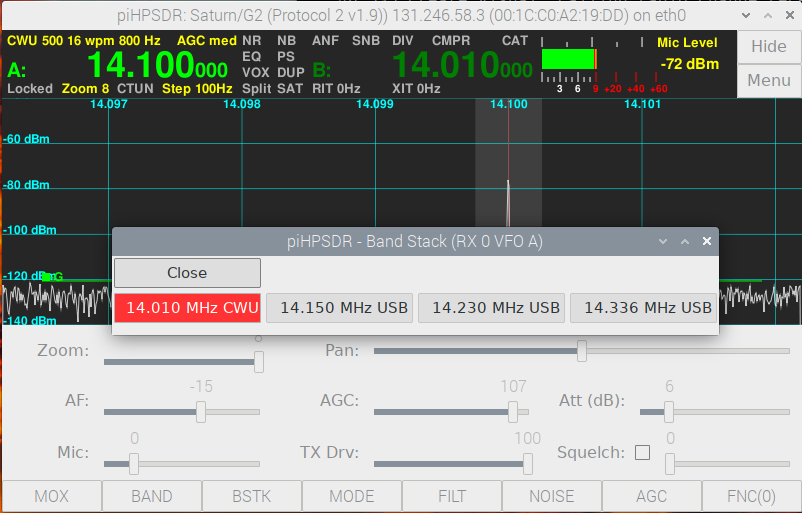
\includegraphics[width=12cm]{BandstackMenu.png}
\caption{The \bltt{BndStack} (Bandstack) menu.}
\label{fig:BandstackMenu}
\end{figure}

For each band, the band stack is collection of operating frequencies/parameters. The idea is that
you can have preferred or recently visited frequencies to which you can easily come back.
The parameters that are actually stored are the frequency, the mode (e.g. USB or FMN),
the filter, and whether CTUN is enabled or disabled. The bandstack parameters
also encompass some FMN-specific parameters,  namely the deviation and
the  CTCSS setting.
If you open the \bltt{BndStack} menu (Fig. \ref{fig:BandstackMenu}), the buttons
tell you about the frequency and the mode, and the band stack entry currently selected is highlighted.

If you press the highlighted button, the parameters which are currently effective are stored in that band stack
entry. If you press another (non highlighted) bandstack button, then first the current
parameters are stored in the highlighted band stack entry, and then the parameters of the
new entry become effective. Note that parameters in bandstack entries are only changed if the active
receiver is controlled by VFO-A.

%%%%%%%%%%%%%%%%%%%%%%%%%%%%%%%%%%%%%%%%%%%%%%%%%%%%%%%%%%%%%%%%%%%%%%%%%%%%%%%%%%%%%%%%%%%%%%%%%%%%%%%%%%%%
\section{The \texttt{Mode} menu}
\begin{figure}[ht]
\center
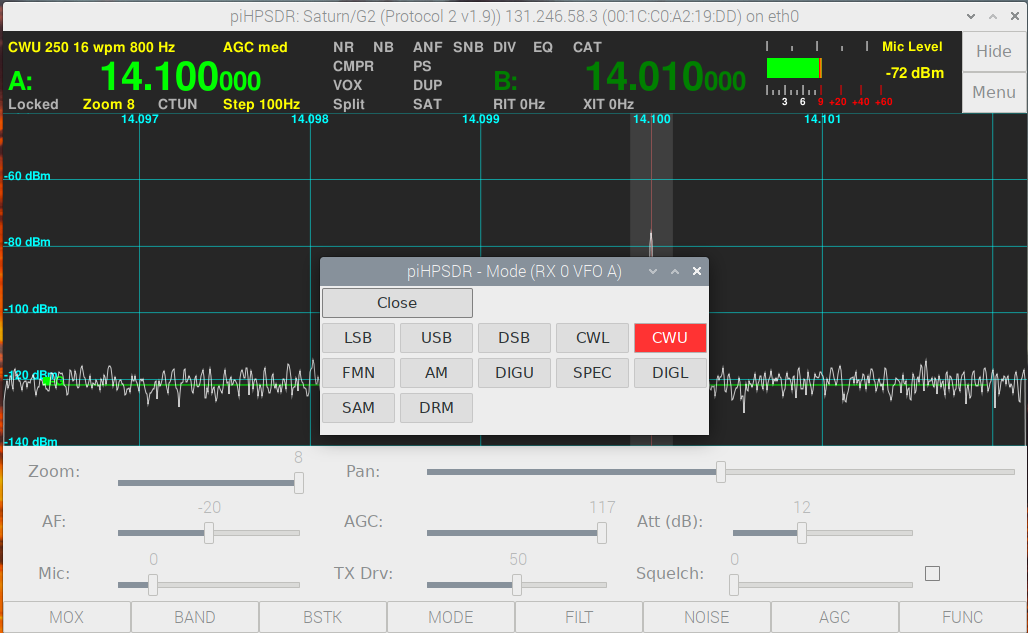
\includegraphics[width=12cm]{ModeMenu.png}
\caption{The \bltt{Mode} menu.}
\label{fig:ModeMenu}
\end{figure}

The \bltt{Mode} menu lets you change the mode of the active receiver, so you can switch,
say, from LSB to CWU or DIGU. The mode menu simply lists the available modes, the current
one is highlighted (Fig. \ref{fig:ModeMenu}).

\textbf{Settings stored with the mode.} Many settings such as filter choices, noise reduction
and equalizer settings, and TX compressor settings
 are only reasonable with a specific mode in mind. Therefore, these settings are stored with
 the mode. If you later switch back to this mode, the settings that were effective the last
 time you used that mode are restored. This is the main reason why the USB and DIGU modes
 are separate (although technically they are the same), the same applies for LSB and DIGL.
 For digital operation, you will normally choose DIGU and have no noise reduction, no TX
 compressore, and no equalizer. For voice operation (USB/LSB) you may then have the
 noise reduction, equalizer and TX compressor settings as you like it. Then you can easily
 switch between DIGU and USB/LSB and have the correct settings automatically. The same applies
 to CWL/CWU where you will normally use different settings compared to both USB/LSB and DIGU.

%%%%%%%%%%%%%%%%%%%%%%%%%%%%%%%%%%%%%%%%%%%%%%%%%%%%%%%%%%%%%%%%%%%%%%%%%%%%%%%%%%%%%%%%%%%%%%%%%%%%%%%%%%%%
\clearpage
\section{The \texttt{Memory}  menu}

The \bltt{Memory} menu gives you access to five memory slots. The menu is shown in Fig. \ref{fig:MemMenu}.
You can store the current
operating frequency  of the active receiver in any of the five slots by clicking a
button in the leftmost columns (e.g. "Store M2"), or you can restore
data from any slot. Parameters stored in the memory slot are
the frequency and the mode, the filter used, the deviation, and the CTCSS setting.
The right column shows the frequency, the mode,
and filter currently stored in the memory slot and clicking on of the five buttons there will restore
the data. So if you have some often used frequencies (e.g. for a net), the
\bltt{Memory} menu allows you to become QRV there with only few mouse clicks.

 \begin{figure}[ht]
\center
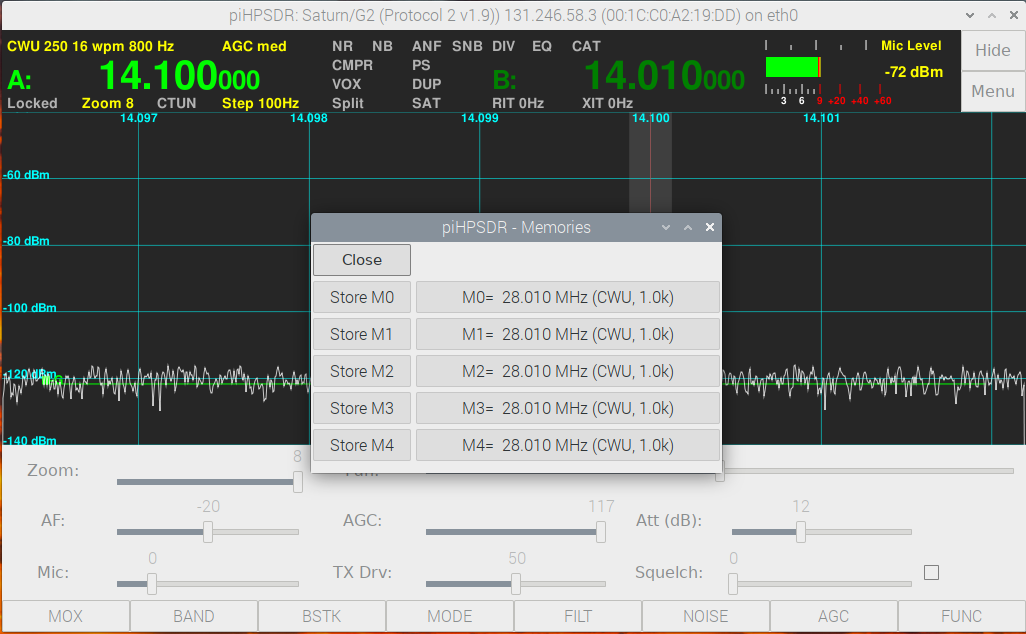
\includegraphics[width=12cm]{MemMenu.png}
\caption{The \bltt{Memory} menu.}
\label{fig:MemMenu}
\end{figure}

%%%%%%%%%%%%%%%%%%%%%%%%%%%%%%%%%%%%%%%%%%%%%%%%%%%%%%%%%%%%%%%%%%%%%%%%%%%%%%%%%%%%%%%%%%%%%%%%%%%%%%%%%%%%
%%%%%%%%%%%%%%%%%%%%%%%%%%%%%%%%%%%%%%%%%%%%%%%%%%%%%%%%%%%%%%%%%%%%%%%%%%%%%%%%%%%%%%%%%%%%%%%%%%%%%%%%%%%%
\chapter{The Main Menu: RX-related menus}

The second column of tghe main menu contains menus which allow you to change
receiver settings.

\section{The \texttt{RX} Menu}

Invoking the \bltt{RX} menu through the main menu always implies that the settings
of the active receiver are to be modified. Using a mouse, you can also open the menu
by a secondary click (using the right mouse button) into the receiver panel. This way,
if piHPSDR is running two receivers, you can open the \bltt{RX} menu for both receivers
(the active receiver as well as the other one), depending on in which panel you have
right-clicked. Note secondary clicks are usually not possible with a touch screen.
The menu is shown in Fig. \ref{fig:RXMenu}.

\rett{Sample Rate} This box is only shown for radios running P2, since only there the
receivers can have an individual sample rate. For radios running P1 or radios accessed
through the SoapySDR library, the sample rate is a global quantity that is modified
throught the \bltt{Radio} menu (see above).

\rett{Select ADC} This box is only shown if the radio has more than one analog-to-digital
converter (ADC), such as Orion, Orion-II and Saturn boards. These radios have two ADCs so
you can choose whether the receiver gets data from ADC0 or ADC1. For these radios, nearly
all antenna jacks go to ADC0, while there is a jack denoted "RX2" (or similar) that
is connected with ADC1. In most cases, ADC0 is used for normal operation, while ADC1
can be used for connecting a dedicated RX antenna.

\textbf{Note: Diversity}. When using \bltt{Diversity} reception, the ADC setting is
overridden, since there data streams from ADC0 and ADC1 are combined (mixed).

\begin{figure}[ht!]
\center
\includegraphics[width=12cm]{RXMenu.png}
\caption{The \bltt{RX} menu.}
\label{fig:RXMenu}
\end{figure}

\rett{Dither}. When checked, the ,,dither'' bit is set which affects the operation of
the ADC converter in some HPSDR boards.

\rett{Random}. When checked, the ,,random'' bit is set which affects the operation of
the ADC converter in some HPSDR boards.

\rett{Preamp}. This checkbox is not shown in Fig. \ref{fig:RXMenu}, it only occurs
for some legacy HPSDR boards which had a switch-able RX preamp.

\rett{Mute when not active}. If checked, the audio from this receiver is muted when
it is not the active receiver.

\rett{Mute audio}. If checked, the audio from this receiver is muted, no matter whether
it is active or not.

\rett{Local Audio Output:} If checked, the audio from this radio is sent to a local
sound card (or virtual audio cable). The sound card itself is selected in the
pop-down menu below this check box. One line below, one can select between
\texttt{STEREO}, \texttt{LEFT} and \texttt{RIGHT}, and select whether the RX
audio should be sent to both channels or to the left or right one only. This way,
one can use one sound device for the first receiver and select LEFT,
and choose another sound device for the second
receiver and choose RIGHT. If one then mixes these two audio streams (either by
operating system facilities or in hardware), one gets the first receiver audio
on the left ear and the second receiver audio on the right ear, which may help
in split operation in DX chasing.

In the example shown, checking the Local Audio box would send the RX audio
samples to the HDMI monitor attached to the RaspPi, but one could equally
well choose the headphone output or a virtual cable, if one wants to use
digital modes.

%%%%%%%%%%%%%%%%%%%%%%%%%%%%%%%%%%%%%%%%%%%%%%%%%%%%%%%%%%%%%%%%%%%%%%%%%%%%%%%%%%%%%%%%%%%%%%%%%%%%%%%%%%%%
\section{The \texttt{Filter} menu}

\begin{figure}[ht]
\center
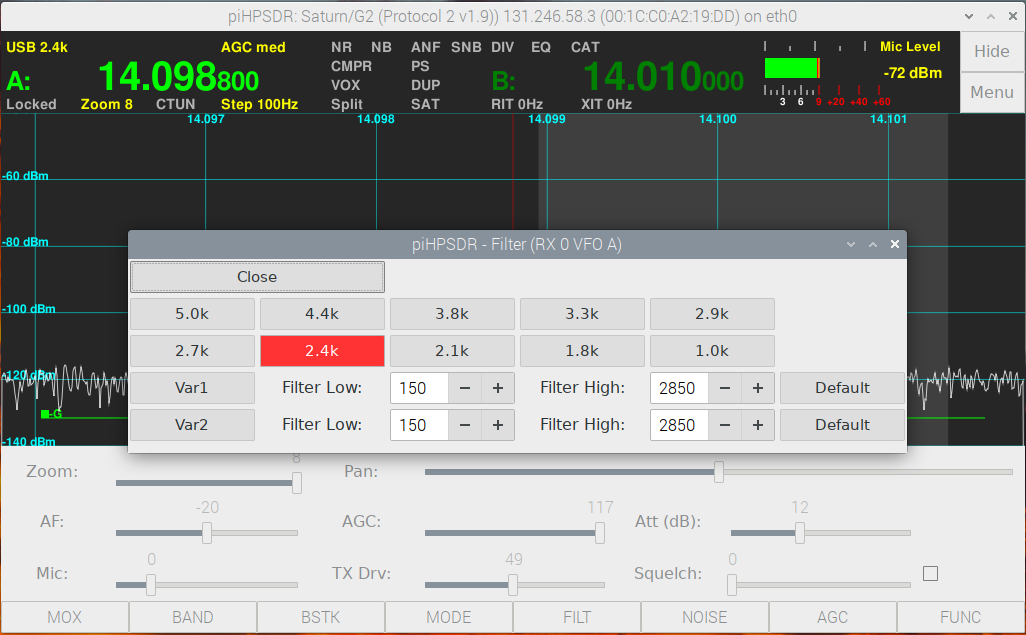
\includegraphics[width=12cm]{FilterMenuUSB.png}
\caption{The \bltt{Filter} menu (single side band modes).}
\label{fig:FilterMenuUSB}
\end{figure}

With the \bltt{Filter} menu, you can change the filter of the active receiver. There
are ten fixed filters and two variable filters, see Fig. \ref{fig:FilterMenuUSB}. It
depends on the current mode which filters are at your disposal, and Fig. \ref{fig:FilterMenuUSB}
is what you see for USB and LSB modes. The filter currently active is highlighted, and
you can choose another filter simply clicking the button. For USB and LSB, the filters
are such the low-frequency cut (in the audio domain) is at 150 Hz, so a 2.7k filter
actually encompasses audio frequencies from 150 to 2850 Hz. With the variable filters
(Var1 and Var2) you can be more flexible in the low audio frequency range. Here you
can individually select the low- and high frequency cut (both frequencies refer to
the audio domain, and are thus both positive value for USB and LSB).

The pre-defined filters for the digital modes DIGU and DIGL are a little bit different.
For filter widths up to 3 kHz, the filter is centered around 1500 Hz. For example,
a 1.0k filter for DIGU/DIGL passes audio frequencies between 1000 and 2000 Hz.

\begin{figure}[ht]
\center
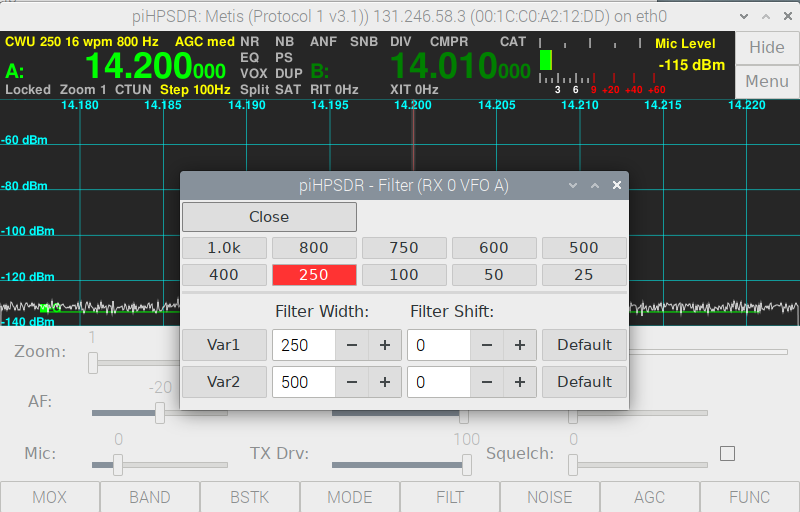
\includegraphics[width=12cm]{FilterMenuCW.png}
\caption{The \bltt{Filter} menu for CWL/CWU.}
\label{fig:FilterMenuCW}
\end{figure}

For modes such as CW and AM, low/high cutoff frequencies have little meaning, so the
\bltt{Filter} menu looks slightly different (Fig. \ref{fig:FilterMenuCW}). The fixed
filters are designated by their width, they are centered around zero (for AM) or around
the CW side tone frequency (for CWU and CWL). For the variable filters Var1 and Var2,
the spin buttons can set the filter width and the filter shift. Normally you will not
want to change the filter shift, but it may help in special cases.

\rett{Enable additional CW Audio peak filter}. If the mode of the
active receiver is CWL or CWU, there will be an addition check box in the
top row of the menu. Here you can enable/disable an audio peak filter that
is applied to the final audio output of the receiver, that is, on top of
the regular filtering. The audio peak filter will only be effective in
the CW modes, its center frequency is given by the CW side tone frequency
and its width is automatically calculated, depending on the
width of the primary filter. The audio peak filter can be used to dig out
the CW signal from the noise (making the regular filter narrower also
does this job). The audio peak filter can also help to tune to the correct
frequency: the regular filters have a flat pass band so the received
signal equally loud as long as it is in the pass band. The audio peak filter
has a marked peak at the side tone frequency so you can tune for maximum
signal volume to adjust your frequency to the received signal.

There is the function \bltt{CW Audio Peak Filter} that can be mapped on toolbar
buttons or GPIO/MIDI buttons so you can quickly enable/disable the audio peak
filter.

\textbf{Filter menu and FM mode.} In FM mode, the \bltt{Filter} menu only lets you
choose between a deviation of 2500 Hz or a deviation of 5000 Hz.
Irrespective of whether the box \rett{Use RX Filter} in the TX menu (see
Chapter \ref{sec:txmenu}) is checked, the deviation setting is used both for RX and TX.
Filter edges (both for
TX and RX) are then calculated according to Carson's rule. Assuming a maximum audio
frequency of 3000 Hz, a filter width of 11 kHz and 16 kHz result for deviations of 2500
and 5000 Hz.

%%%%%%%%%%%%%%%%%%%%%%%%%%%%%%%%%%%%%%%%%%%%%%%%%%%%%%%%%%%%%%%%%%%%%%%%%%%%%%%%%%%%%%%%%%%%%%%%%%%%%%%%%%%%
\section{The \texttt{Noise} Menu}

\begin{figure}[ht]
\center
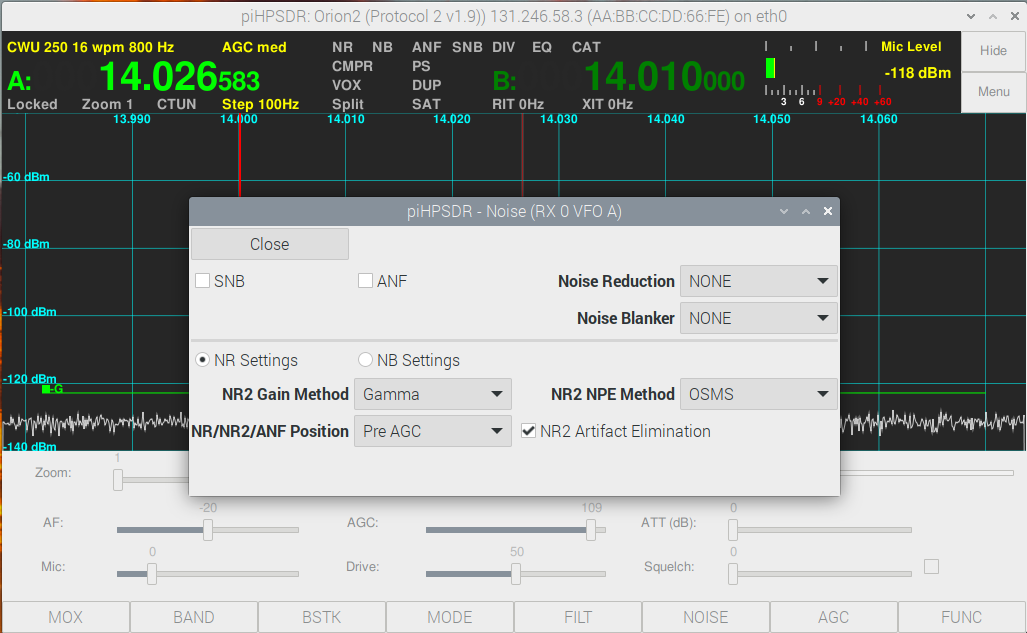
\includegraphics[width=12cm]{NoiseMenu1.png}
\caption{The \bltt{Noise} menu (with NR settings).}
\label{fig:NoiseMenu1}
\end{figure}

With the \bltt{Noise} menu you can select a variety of noise reduction and/or
noise blanker capabilities (Fig. \ref{fig:NoiseMenu1}). The upper part of the
menu always looks the same, the lower part lets you fine-tune noise reduction
or noise blanker parameters. For an in-depth explanation of the noise reduction
and noise blanker capabilites, the reader is referred to the WDSP manual.

\rett{SNB} This check box lets you enable/disable the spectral noise blanker.

\rett{ANF} This check box enables/disables the automatic notch filter. The ANF is
very good at eliminating a single-tone QRM carrier in SSB modes. It goes without
saying that activating the ANF in CW is detrimental rather than beneficial, because
here the signal is of the type the ANF tries to eliminate.

\rett{Noise Reduction} With this pop-down menu, you can choose the type of noise reduction
(no noise reduction, NR1 or NR2).

\rett{Noise Blanker} With this pop-down menu, you can choose the type of noise blanker
(no noise blanker, the preemptive wideband blanker NB or the interpolating widetband
blanker NB2 ).

\rett{NR Settings/NB Settings} Choosing one of the two buttons determines whether the
lower part of the menu offers fine-tuning of the noise reduction or noise blanker settings.
The set up for changing the noise reduction settings is shown in Fig. \ref{fig:NoiseMenu1},
below (Fig \ref{fig:NoiseMenu2}) you find the set up for changing the noise blanker settings.
We discuss the noise reduction settings first, but note again for the details you have
to study the WDSP manual.

\rett{NR2 Gain Method} The available choices for the NR2 noise reduction here are Linear, Log, and Gamma, where Gamma is the default.

\rett{NR2 NPE Method} The available choices for the NR2 noise reduction here are OSMS and MMSE,
where OSMS is the default.

\rett{NR...Position} In the RX chain, the noise reduction can be placed before or after
the automatic gain control (AGC). The choice here refers to \textit{all} noise reduction
capabilities (SNB, ANF, NR1, NR2).

\rett{NR2 Artifact Elimination} The NR2 noise reduction algorithm is prone to producing
artifacts, so there is an option to reduce such artifacts which should normally be checked
(artifact elminiation ,,on'').

\begin{figure}[ht]
\center
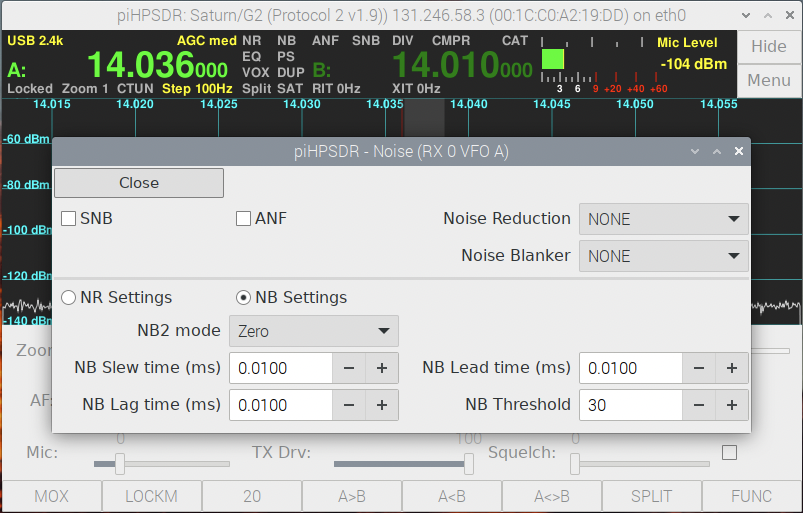
\includegraphics[width=12cm]{NoiseMenu2.png}
\caption{The \bltt{Noise} menu (with NB settings).}
\label{fig:NoiseMenu2}
\end{figure}

Note the noise blanker works very different from the noise reduction, since noise blanking
is applied to the original RX IQ samples before any frequency shifts etc. take place.
If you have a single source of noise (e.g. a Plasma TV) that drives you crazy, it is worth
the effort to play around with the NB2 parameters, especially the timings. Different
QRM sources will require different parameters! The default parameters have been proven useful
for many situations, but for you a different setting may produce better results!
The options to control the noise blanker algorithms are:

\rett{NB2 Mode} The available choices for the interpolating NB2 noise blanker here are Zero,
Sample\&Hold, Mean Hold, Hold Sample, and Interpolate.

\rett{NB Slew time/Lag time/Lead time/Threshold} These parameters apply both to NB and NB2.
piHPSDR currently does not allow to have a separate set of parameters for NB and NB2.


%%%%%%%%%%%%%%%%%%%%%%%%%%%%%%%%%%%%%%%%%%%%%%%%%%%%%%%%%%%%%%%%%%%%%%%%%%%%%%%%%%%%%%%%%%%%%%%%%%%%%%%%%%%%
\section{The \texttt{AGC} Menu}

Only few parameters can be controlled via the automatic gain control (AGC) menu.
The first is the AGC time constant, which can be Off (no AGC), Long, Slow, Medium,
and Fast. A very long AGC time constant protects your ears, but it also means that
the receiver becomes ,,deaf'' for a rather long time after a strong QRM burst. This
phenomenon is known as "AGC pumping". Generally, if you do SSB on a quiet band, the
AGC time constant can be longer, for CW on the other hand, I personally prefer short
time constants (Medium or Fast).

The \rett{AGC Hang Threshold} is only effective if the AGC time constant is Long or Slow,
since the AGC hang time is turned off for Medium and Fast.
In this case, the RX spectrum scope not only shows the ,,normal'' AGC line in green,
but also the hang threshold line in orange.

\begin{figure}[ht]
\center
\includegraphics[width=12cm]{AGCMenu.png}
\caption{The \bltt{AGC} menu.}
\label{fig:AGCMenu}
\end{figure}

%%%%%%%%%%%%%%%%%%%%%%%%%%%%%%%%%%%%%%%%%%%%%%%%%%%%%%%%%%%%%%%%%%%%%%%%%%%%%%%%%%%%%%%%%%%%%%%%%%%%%%%%%%%%
\section{The \texttt{Diversity} Menu}

\bltt{Diversity} is a very powerful tool to improve reception by using two different
antennas and two ADCs. To explain how it works, suppose you live in a house which produces
a lot of local QRM. Your ,,normal'' antenna will pick up the wanted DX signals, but also
a lot of noise that originates somewhere in your house. Now suppose you have a second
receive-only antenna placed in your house that will predominantly pick up your local
QRM and only very little DX signal.

\begin{figure}[ht]
\center
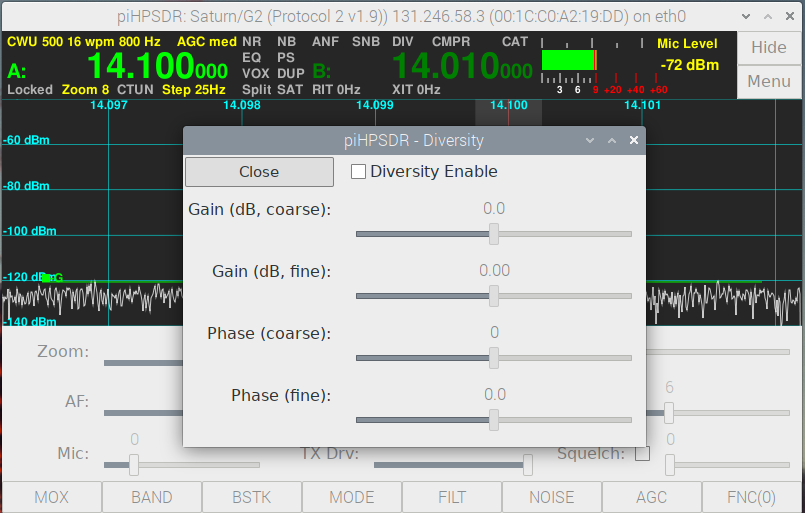
\includegraphics[width=12cm]{DiversityMenu.png}
\caption{The \bltt{Diversity} menu.}
\label{fig:DiversityMenu}
\end{figure}

Of course, this RX-only antenna does not deliver anything useful at first sight. But, imagine
you could shift the phase and the amplitude of the signal of the in-house antenna such that it
exactly opposes the local QRM picked up by your DX antenna! Adding this (phase shifted and amplitude
adjusted) signal from your in-house antenna to what comes from your DX antenna will produce
a signal where the local QRM is largely eliminated while the DX signal is only weakly affected.
This is what \bltt{Diversity} is all about.

%%%%%%%%%%%%%%%%%%%%%%%%%%%%%%%%%%%%%%%%%%%%%%%%%%%%%%%%%%%%%%%%%%%%%%%%%%%%%%%%%%%%%%%%%%%%%%%%%%%%%%%%%%%%
%%%%%%%%%%%%%%%%%%%%%%%%%%%%%%%%%%%%%%%%%%%%%%%%%%%%%%%%%%%%%%%%%%%%%%%%%%%%%%%%%%%%%%%%%%%%%%%%%%%%%%%%%%%%
\chapter{The Main Menu: TX-related menus}

Note that for RX-only radios, only the \bltt{CW} menu will be shown here
because there one can set the pitch of the CW side tone, which also affects
the RX ,,BFO frequency''.

\section{The \texttt{TX} Menu}
\label{sec:txmenu}
\begin{figure}[ht!]
\center
\includegraphics[width=12cm]{TXMenu.png}
\caption{The \bltt{TX} menu.}
\label{fig:TXMenu}
\end{figure}

The \bltt{TX} menu can be opened from the main menu, or just by a secondary mouse click
into the TX panadapter (while transmitting). The menu is shown in Fig. \ref{fig:TXMenu}.


\rett{Local Microphone}. If this box is checked, the TX audio samples come from a soundcard
attached to the host computer, or from a virtual audio cable. The sound device can be
selected from the pop-down menu to the right.
 This check box, and the pop-down menu, is absent if
there are no output sound devices available.

\textbf{Note:} If the radio has the possiblity
to connect a microphone, and if PTT comes from the radio, the radio microphone samples
and the local (sound device) microphone samples are mixed (added). This is very convenient
if one does SSB with a microphone attached to the radio, and digital modes with a
local sound device or virtual audio cable: when doing SSB, the local sound device normally
produces no audio, and while pressing PTT at the microphone, you can work SSB normally.
So you can go from digital mode to SSB without the need to change the microphone setup
in the TX menu.

\rett{Compression (dB):} With this box the TX compressor can be enabled/disabled.
The compression level (0-20 dB) can be chosen in the spin button to the right.

\textbf{Note:} The compressor on/off flag, as well as the compression level, is
,,stored with the mode''. So it is possible to have the compressor enabled for SSB
(LSB/USB)
and disabled for digi modes (DIGL/DIGU), and when switching modes, the compressor
settings for the new mode are automatically restored.

\rett{FM PreEmp/ALC}. When transmitting FM, the audio input signals are ,,emphasized''.
This means that from 300 to 3000 Hz (the usual range of audio frequencies in amateur
radio FM), there is a 6 dB per octave (20 dB per decade) that leads to a 20 dB damping
of an input signal at 300 Hz (8 dB damping at 1200 Hz, and no damping ad 3000 Hz).
This of course distorts the audio, but the reverse process is built into FM demodulators
to correct for this. Because there is a lot of damping of the audio signal, piHPDSR
applies a 15 dB boost to the TX audio input samples when the mode is FMN.

This boost is nearly ineffective if the FM pre-emphasis takes place \textit{after}
the TX ALC stage, since the ALC will cancel most of the extra boost and the FM
modulation sounds ,,thin''. If the \rett{FM PreEmp/ALC} box is checked, FM
pre-emphasis takes place \textit{before} the TX ALC, such that the ALC ,,sees''
the TX audio input after applying both the boost and the damping of the pre-emphasis. This gives the
transmitted signal a little more ,,punch''. It is generally recommended to have this box checked
if doing FM.

\rett{Radio Mic:} This text, and the pop-down menu to its right, only occurs if a microphone can
be connected to the radio. The pop-down menu lets you choose between \rett{Mic In} which means
that a microphone can be connected to the microphone input jack, \rett{Mic Boost}, which
additionally switches on a hardware 20 dB mic amp, and \rett{Line In} which means that the
"Line In" jack of the radio is used for the audio samples transferred from the radio to the
host computer. This is part of the HPSDR protocol, it may well happen that your radio has a
microphone jack but no line-in input. The optional 20 dB preamp may be necessary when connecting
a dynamic microphone whose input level (few mV) is considerably lower that that of a
condensor (electret) microphone, or a dynamic microphone with built-in preamp.

\rett{TX Filter low:} With this spin button you can set the low cut of the TX filter. The
frequency refers to the audio domain.

\rett{TX Filter high:} With this spin button you can set the high cut of the TX filter. The
frequency refers to the audio domain.

\rett{Use RX Filter} If this check box is enabled, the TX filter low/high cuts are ignored,
and the filter edges of the current RX filter are used instead.

\rett{Panadapter Low:} This spin button sets the lower edge (in dBm) of the TX panadapter.

\rett{Panadapter High:} This spin button sets the upper edge (in dBm) of the TX panadapter.

\rett{Panadapter Step:} This spin button determines how many horizontal lines are drawn on the
TX panadapter. If set to 10, for example, there will be a horizontal line for every multiple
of 10 dBm.

\rett{AM carrier level:} This sets the AM carrier level for the AM modulator. If set to zero, there is no
carrier and the
signal is a DSB signal. A reasonable value is 0.5 which leads to 100\% modulation. Values larger than
0.5 have less than 100\% modulation. This means too much power goes into the carrier.

\rett{Tune use Drive} If this box is checked, TUNEing will be done with the power that corresponds to the
current position of the drive slider, and the tune drive level is ignored.

\rett{Tune Drive Level} The value that can be adjusted with this spin box is the virtual position of the
drive slider while TUNEing. This value is ignored if the \rett{Tune use Drive} box is checked.

\rett{SWR protection} If this box is checked, a very simple SWR protection is enabled. If the SWR exceeds
the threshold value (see next point), the drive slider is set to zero. The SWR protection is disabled
while TUNEing.

\rett{SWR alarm at} The spin button to the right determines the SWR threshold. If the SWR is beyond the
threshold, the SWR reported in the meter turns red. If SWR protection is enabled, the drive slider is set to
zero if the SWR exceeds the threshold.

\rett{CTCSS Enable} (FM only!) This checkbox enables/disables CTCSS (continuous tone coded squelch system).
If enabled, a low-frequency
tone is transmitted together with the normal TX audio. This can be used to trigger repeaters, or any other
function implemented
on the other side. The frequency itself can be chosen with the following menu point:

\rett{CTCSS Frequency} This pop-down menu lets you choose the CTCSS frequency. This choice has no effect if
CTCSS is disabled.
The frequency list includes 38 standard TIA/EIA-603-D CTCSS frequencies between 67.0 and 250.3 Hz.

\rett{Mac Drive level for DIGU/DIGL} This spin button restricts the range of the drive slider from 0 to the
chosen value
for the DIGU and DIGL modes. If the value is 100, this has no effect. The primary use of this menu point is
PA protection,
since many digital modes (unlike SSB voice) are constantly transmitting at full power.

%%%%%%%%%%%%%%%%%%%%%%%%%%%%%%%%%%%%%%%%%%%%%%%%%%%%%%%%%%%%%%%%%%%%%%%%%%%%%%%%%%%%%%%%%%%%%%%%%%%%%%%%%%%%
\section{The \texttt{PA} Menu}

In the \bltt{PA} menu, you can adjust the output level of your HPSDR board
to the PA being used, and you can establish a calibration of the
power begin displayed in the meter section while transmitting.
The menu presents itself as shown in Fig. \ref{fig:PAMenuCalibrate}.

\begin{figure}[ht]
\center
\includegraphics[width=12cm]{PAMenuCalibrate.png}
\caption{The PA menu, PA calibration screen}
\label{fig:PAMenuCalibrate}
\end{figure}

In the first line, you can choose the maximum PA power of your
radio. The available values are 1, 5, 10, 30, 50, 100, 200, and
500 Watt. If your radio has a different maximum power, choose the
next largest value. The choice of this value only affects the
watt meter calibration (see below). If the  box
\rett{Transmit out of band} is checked, this allows piHPSDR
to go TX if you are outside of the amateur radio bands.



\textbf{PA calibration.} If the \rett{Calibrate} sub-menu is active
(as shown in Fig. \ref{fig:PAMenuCalibrate}) you can adjust your
HPSDR board to your PA. This has to be done for each band separately,
and you need a dummy load and a watt meter to do so. Most watt meters
used by radio amateurs are not highly accurate, so if you can borrow
an accurate one, do so. The PA calibration values are the fictious
amplification of the PA. If the value is \textit{increased},
piHPSDR assumes a higher amplification and will thus \textit{decrease}
the output power of the HPSDR board. Thus, \textit{increasing} the
PA calibration value will \textit{decrease} the output power. A calibration
value of 38.8 dB corresponds to the maximum RF output of the HPSDR board,
so the allowed range of values starts at 38.8.

To start calibration, go to the \bltt{TX} menu and check the
box \rett{Tune use Drive}. Then, hit the rightmost toolbar button
until one of these buttons reads \bltt{TUNE}. This way, when
TUNEing, you send a carrier with the power according to the drive
slider. For each band, go to the middle of the band, open the PA
menu, put the drive (\rett{TX Drv}) slider at 50 and hit the TUNE button. If the
output (measured with the Watt meter) is higher than half
 of your nominal PA power, increase the
PA calibration value of that band, otherwise decrease it. Choose
a value such that your Watt meter reads half the nominal output
power. For fine adjusting, move the drive slider to 100 and
adjust the PA calibration value until your Watt meter shows the
nominal output  power. The calibration values will  (slightly)
differ from band to band, often one needs smaller values for the
higher bands since the amplification of the PA is smaller there.
If transverter bands have been defined via the \bltt{XVTR} menu,
they will also show up in this menu. Note that the PA calibration
value affects the level of the low-power TX output of the HPSDR board
an thus affects both the PA output (if the PA is enabled) as well
as the low-power TX output (if the Xvtr port is active as RX antenna).

\textbf{Watt meter calibration.} When PA calibration is complete,
you can calibrate the power reading within the meter section of
the piHPSDR window. If you open the \bltt{PA} menu and click
on the text \rett{Watt Meter Calibrate}, the menu changes
and looks like in Fig. \ref{fig:PAMenuWatt}.

\begin{figure}[ht]
\center
\includegraphics[width=12cm]{PAMenuWatt.png}
\caption{The PA menu, Watt meter calibration}
\label{fig:PAMenuWatt}
\end{figure}

You have 10 Watt values from $\frac{1}{10}$ to the full nominal power. Initially,
the values of the spin buttons beside the Watt ratings have the nominal value.
The calibration values can always be re-set to these nominal values by hitting
the \rett{Reset} button. Watt meter calibration is not done seperately for all
bands, so it is suggested to perform the following procedure on the 20m band.
piHPSDR will convert the ,,measured'' into the ,,reported'' value by linear
interpolation between two adjacent calibration values.

Start with resetting the value by hitting the \rett{Reset} button. Then, move the
drive slider to 100 (the unit of the drive slider is per cent, not Watt!) and hit
TUNE. After the PA calibration described above, your (external) Watt meter should
show the nominal PA output power (e.g. 100 Watt for an ANAN-7000). Now look at the
forward power reported in the meter section (top right of the piHPSDR window).
Suppose you read "250 W" there although your output is 200 Watt. Then simply
insert the number 250 in the spin button to the right of the string
\rett{200W}. Now your watt meter reading should be close to 200W, you can fine-tune
it with the spin button. Note that \textit{increasing} the calibration value
with the spin button will \textit{decrease} the power indicated in the meter section.

You will observe that the calibration values for the lower powers also have changed.
This only happens if you start from nominal calibration values and change the
calibration value of the highest power. For example, if you have entered 250 in
the 200W spin button, then the value in the 100W spin button will read 125. So in a
single shot, you have roughly calibrated the Watt meter.

A finer calibration only makes sense if you have a highly accurate Watt meter. If you do,
you can now move the drive slider until your Watt meter exactly reads one of the
lower power values, and use the corresponding spin button to change the calibration
until piHPSDR exactly reports the correct power.

The procedures is the virtually the same if our nominal output power is different.
The only complication arises if your radio has a nominal power that is not in the menu,
for example 150 Watt.

In this case, choose 200W in the top line of the PA menu. TUNE and move the drive
slider until your Watt meter reads the largest value possible that occurs
in the Watt meter calibration menu (in this example, it is 140W). Adjust the
140W spin button until piHPSDR reports 140 Watt. Then go to full power
(150W) and adjust the 200W spin button until piHPSDR reports 150 Watt.
Then, proceed with 120, 100, 80, etc. Watts.

%%%%%%%%%%%%%%%%%%%%%%%%%%%%%%%%%%%%%%%%%%%%%%%%%%%%%%%%%%%%%%%%%%%%%%%%%%%%%%%%%%%%%%%%%%%%%%%%%%%%%%%%%%%%
\section{The \texttt{VOX} Menu}

VOX (voice control) means that you can just speak into the microphone and the
radio goes TX, without the need to press a PTT button. VOX can also be used
in digital modes, if there is no possiblity that the digimode program can
put piHPSDR into TX mode via CAT commands or hardware lines. The VOX menu
is shown in Fig. \ref{fig:VOXMenu}.

\begin{figure}[ht]
\center
\includegraphics[width=12cm]{VOXMenu.png}
\caption{The VOX menu}
\label{fig:VOXMenu}
\end{figure}

With the \rett{VOX Enable} check box, you can enable/disable VOX. For VOX operation,
there are two parameters, namely the VOX threshold and the VOX hang time. The VOX threshold
is the microphone amplitude required to trigger a RX/TX transition. If the radio goes TX
when the neighbour's hound starts barking, then the VOX threshold is too small. If the radio
does not go TX  although you speak loudly into the microphone, the threshold is too large.
The VOX menu features an indicator which can be green or red (in Fig. \ref{fig:VOXMenu}, this
is the green bar). This indicator flashes red if the microphone amplitude is above the VOX
threshold. Adjust the threshold with the slider such that the indicator becomes red if  you
speak into the microphone, but stays green if you don't speak.

The VOX hang time determines how long the radio stays in TX mode after the last time the
microphone delivered a signal that was above the VOX threshold. Typical values are 250 to
500 milli seconds. If your radio produces relay chatter because it goes RX between your words,
increase the hang time. However, this will also increase the turn-around between you finished
your message and go RX.

VOX is very nice for rag-chew phone QSOs, I won't recommend it for contest operation.

%%%%%%%%%%%%%%%%%%%%%%%%%%%%%%%%%%%%%%%%%%%%%%%%%%%%%%%%%%%%%%%%%%%%%%%%%%%%%%%%%%%%%%%%%%%%%%%%%%%%%%%%%%%%
\section{The \texttt{PS} (PureSignal) Menu}

\begin{figure}[ht]
\center
\includegraphics[width=12cm]{PSMenu.png}
\caption{The PureSignal (PS) menu}
\label{fig:PSMenu}
\end{figure}

PureSignal is the ,,street name'' for adaptive pre-distortion. What this means is, that
the signal from the \textit{output} of the PA (the ,,antenna signal'') is coupled
back (through an attenuator of typically 40-60 dB) to the radio and is analyzed
whether is looks like it should. If it is distorted (e.g. by non-linearities of the PA),
then the PureSignal algorithm calculates how an input signal to the PA should look like
to produce the desired output. This is usually measured and calibrated with a so-called
two-tone experiment. In this experiment, two constant carriers, for example 7100 kHz
and 7101 kHz, are transmitted. If both carriers contain 25W power, this is
a 100W PEP signal. Non-linearities of the PA first lead to the occurence of harmonics
(in this case around 14.2, 21.3, and 28.4 MHz). This is not a problem because
such harmonics are  damped by the TX low-pass filters. Higher-order non-linear effects,
however, lead to additional in-band signals, in our example they occur at
7102/7099, 7103/7098 etc. kHz. The low-pass filters cannot eliminiate these signals,
they lead to unwanted signals (,,splatter'') that disturb QSOs on neighbouring
frequencies. With PureSignal, you can greatly reduce these un-wanted signals.
If you open the \bltt{PS} menu for the first time it looks like shown in Fig.
\ref{fig:PSMenu}.



The elements have the following function:

\rett{Enable PS} With this check box, PS can be enabled/disabled.

\rett{Two Tone} With this button, a two-tone experiment can be started/stopped. The button
will be highlighted as long as the two-tone signal is transmitted.

\rett{Auto Attenuate} This enables/disables automatic adjustment of the RF input
attenuator to give the feedback level the correct strength. It is highly recommened
to use this option.

\rett{OFF} With this button, the PS correction can be stopped (the \rett{status} will
then change to RESET).

\rett{Restart} With this button, the PS correction can be resumed, for example after
it has been stopped.

\rett{MON} With this button, it can be chosen whether the TX spectrum scope shows
the signal sent to the PA (MON button not highlighted) or whether the feedback signal
from the antenna is shown (MON button highlighted).

\rett{PS Feedback ANT} Here it must be specified which antenna jack is used for the
PS feedback signal. It can be \rett{Internal} which means internal feedback
(for example as built into the Anan-7000 or  simply the cross-talk from the
TX/RX relay), or it can be \rett{Ext1} or \rett{ByPass} which refers to the
auxiliary antenna jacks.

\begin{figure}[ht]
\center
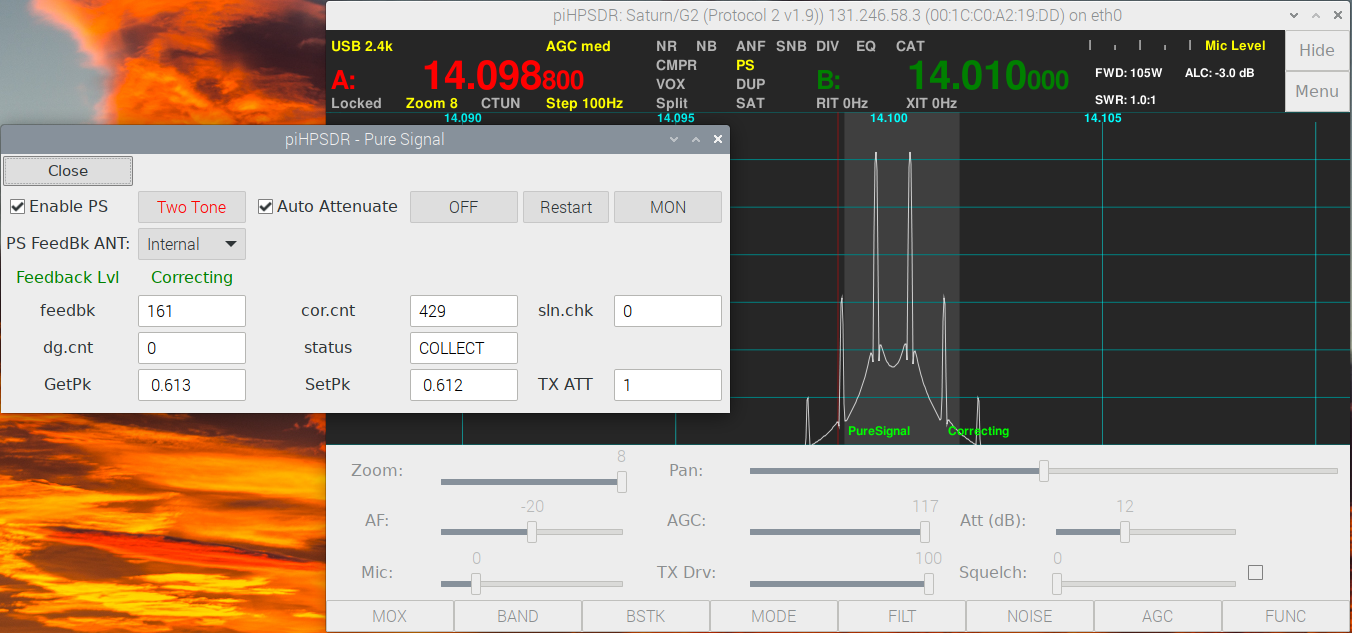
\includegraphics[width=12cm]{PSnomon.png}
\caption{PS: TwoTone without MON}
\label{fig:PSnomon}
\end{figure}

\rett{Feedback Lvl} When doing a PS calibration through a two-tone experiment, this string
turns red if the feedback level is good. It turns yellow if the feedback level is slightly
to weak and read if it is too weak. A blue colour indicates a too string feedback level.
The feedback level reported by the PS calibration algorithm is further reported in the
,,feedbk'' field. The optimum value is about 154.

\rett{Correcting} When doing a PS calibration through a two-tone experiment, this string
is green if calibration was successful and PS correction takes place, and the string is
red if no good calibration could be made.

\begin{figure}[t!]
\center
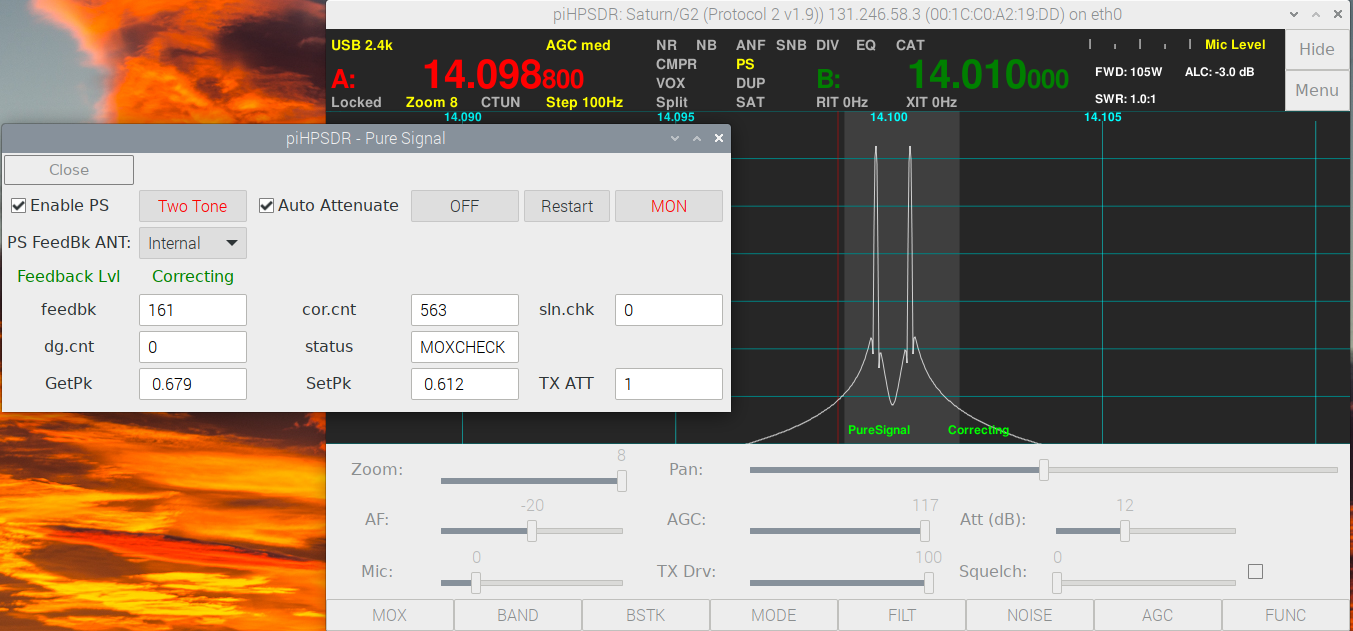
\includegraphics[width=12cm]{PSmon.png}
\caption{PS: TwoTone with MON}
\label{fig:PSmon}
\end{figure}

\rett{TX ATT} If \rett{Auto Attenuate} is not enabled, this is a spin button with which
you can manually adjust the RF attenuation. For normal HPSDR radios, this is a value
between 0 and 31, other radios such as the HermesLite have an extended range from
-29 to 31. If the feedback level is too strong, this value must be increased, if it
is too strong, it must be decreased. It is, however, recommended to enable \rett{Auto Attenuate}.
In this case, the \rett{TX ATT} just shows the current attenuation.

\rett{SetPk} This field shows the currently assumed value of the peak value of the TX DAC
feedback signal. piHPSDR chooses is automatically. It should match the value reported
by the calibration algorithm in the GetPk field. The  value
chosen by piHPSDR can be incorrect if you use a highly experimental firmware on your
HPSDR board with modified TX DAC filters, but this should normally not happen.

\begin{figure}[t!]
\center
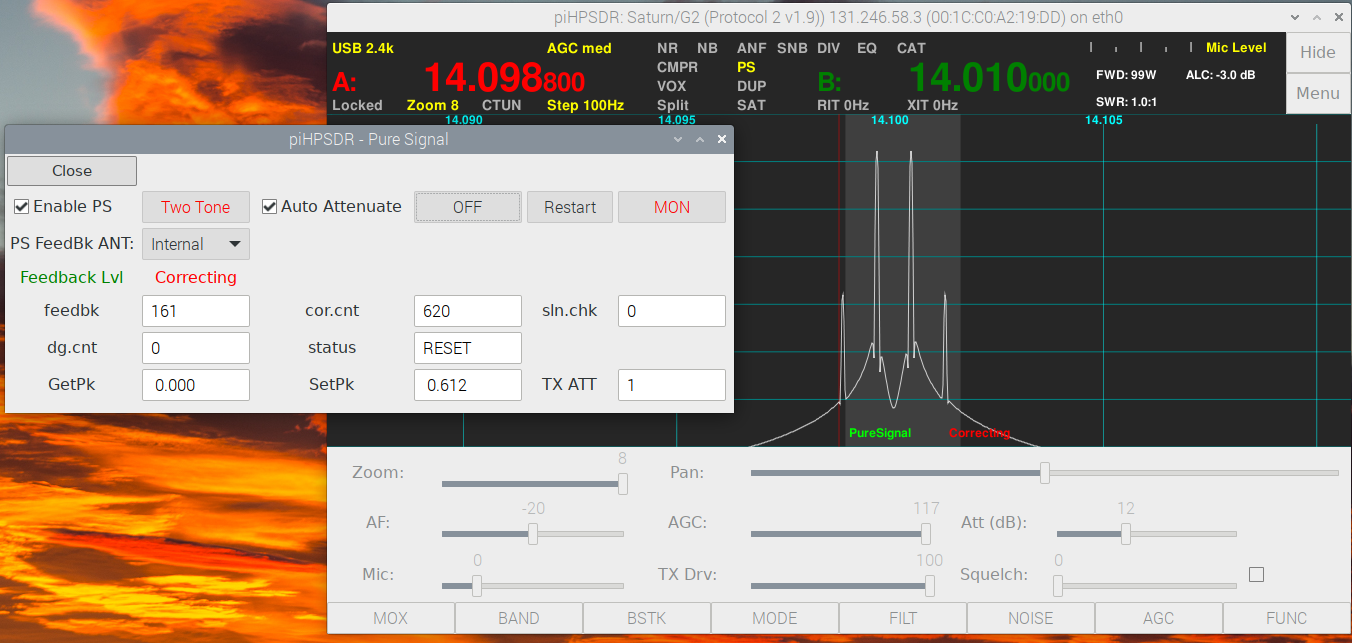
\includegraphics[width=12cm]{PSoff.png}
\caption{PS: after hitting OFF}
\label{fig:PSoff}
\end{figure}

To demonstrate what happens, I show an example. Checking both \rett{Enable PS} and
\rett{Auto Attenuation}, and hitting the \rett{Two Tone} button, it need few
seconds to stabilize and then Fig. \ref{fig:PSnomon} resulted, where the TX
spectrum scope and the PS menu window have been arranged such that they do
not cover each other. Although both the PS menu and the spectrum scope state
that PS is working and correcting, the signal does not look as a good two-tone
signal which would only have two peaks! The reason is, that the TX spectrum scope
normally shows the signal that is sent to the PA, so we see a distorted signal.
However this distortion is magically exactly such that the PA makes a nice signal
out of this. If one wants to see what one is actually transmitting, one must
push the \rett{MON} button such that it is highlighted. Then one sees that
the feedback signal that shows what is going on at the antenna (Fig. \ref{fig:PSmon}):



Here one sees that the antenna emits a clean two-tone signal (no satellites can be seen,
the IM3 value is better than 50 dBc). To demonstrate how effective the PS algorithm is,
I have pushed the \rett{OFF} button which stops the PureSignal calibration, the result
is shown in Fig. \ref{fig:PSoff}. Here we see two satellites with an IM3 value of
about 30 dBc, which reflects the non-linearity of the PA.

%%%%%%%%%%%%%%%%%%%%%%%%%%%%%%%%%%%%%%%%%%%%%%%%%%%%%%%%%%%%%%%%%%%%%%%%%%%%%%%%%%%%%%%%%%%%%%%%%%%%%%%%%%%%
\section{The \texttt{CW} Menu}
The CW menu controls parameters related to CW operation. The menu
is shown in Fig. \ref{fig:CWMenu}.

\begin{figure}[ht]
\center
\includegraphics[width=12cm]{CWMenu.png}
\caption{The CW menu}
\label{fig:CWMenu}
\end{figure}

Many radios have a connection for a paddle or at least for
a straight key, and contain firmware to do CW. CW handling by
the radio firmware is enabled by the \rett{CW handled in Radio}
check box. If unchecked, CW (that is, generating and forming
the RF pulses) is done by piHPSDR, which implies that
a Morse paddle, straight key or an external keyer is connected
to the host compute (see Appendix \ref{sec:ConnectCW}).

\rett{CW Speed}. Here the speed (in wpm) can be chosen. If CW is
handled in the Radio, the value is simply sent to the radio firmware,
which implements the (iambic) keyer. If CW is done within piHPSDR,
this value is used by piHPSDR's built-in iambic keyer. If using
a straight key, or an external keyer whose output is then treated
like a straight key, the speed has no meaning.

In either case, this speed is operative when sending CW text via
CAT commands (KY comand), and it can also be changed by CAT
(KS command).

\rett{CW Break-In} This implements some sort of ,,CW-VOX''. In
break-in mode, the radio is automatically switched to TX when
a key or paddle is pressed. The delay, to be set by the spin
button to the right, is the time the radio goes RX after the
last Morse key closure.

\rett{Sidetone Level}. This is the level of the side tone,
either generated by the radio (if CW is handled there and the radio
has an audio codec) or
by piHPSDR (if CW is not handled in the radio). The allowed range
is 0-255 (P1) or 0-127 (P1 or SoapySDR).

\rett{Sidetone Freq}. This is the frequency of the side tone and the
,,BFO offset''. That is, if a CW signal is received exactly at the
frequency one transmits on, the CW audio signal has this pitch.

\rett{Weight:} If using a iambic keyer (either in the radio or
the builtin keyer), this value (0-100) determines the dash/dot ratio.
The normal value is 50, which means that a dash is three times longer
than a dot. The dash length is proportional to this value, so it can
be from zero to six times the dot length.

\rett{Paddle Mode:} Here the choice is Iambic Mode A, Iambic Mode B,
and  Straight Key. In Straight Key mode, the key has to be connected
to the dash paddle, since the built-in keyer implements a bug mode
there (automatic dots from the dot paddle, straight key behaviour
for the dash paddle). When using an external keyer, use StraightKey
mode and connect the keyer output to the dash paddle input.

\rett{Keys reversed} When checking this box, the dot and dash contacts
are reversed.

\rett{Enforce letter spacing} This option forces you to give ,,cleaner'' CW
when in iambic mode. If at the end of an inter-element pause no key is
pressed, then there is a forced pause of two times a dot length. While this
prevents you from sending too short spaces between two letters, this
might also corrupt a letter you want to send. For example, when sending
the letter "X" and the dot paddle is pressed a little too late, you
instead send "TU". This option might be good for practising, but
I personally never use it.

%%%%%%%%%%%%%%%%%%%%%%%%%%%%%%%%%%%%%%%%%%%%%%%%%%%%%%%%%%%%%%%%%%%%%%%%%%%%%%%%%%%%%%%%%%%%%%%%%%%%%%%%%%%%
%%%%%%%%%%%%%%%%%%%%%%%%%%%%%%%%%%%%%%%%%%%%%%%%%%%%%%%%%%%%%%%%%%%%%%%%%%%%%%%%%%%%%%%%%%%%%%%%%%%%%%%%%%%%
\chapter{The Main Menu: menus for RX and TX}

\section{The \texttt{DSP} (Signal Processing) Menu}

\begin{figure}[ht]
\center
\includegraphics[width=12cm]{DSPMenu.png}
\caption{The DSP menu.}
\label{fig:DSPMenu}
\end{figure}

The \bltt{DSP} menu sets parameters related to DSP (digital signal processing)
within the WDSP library.
Filter characteristics can be specified separately for the RX1 (and RX2, if
running two receivers) and TX (if the radio does have a transmitter)
filters. In addition, enabling/disabling binaural receiver audio
is done here.  Most users will
very rarely need to invoke this menu, which is shown
in Fig. \ref{fig:DSPMenu}.

\rett{Filter Type}. Digital filters can be designed such that a signal within the
passband leaves the filter in a shape as similar as possible
to what went into the filter. This requires that the phase
difference between input and output signal is a linear
function of the frequency. Another desirable property
of a linear filter is that the time delay between a signal
going into a filter and what comes out is as small as
possible. Unfortunately there some sort of uncertainty
relation between these two properties, so you only can
trade one for the other. The options for the filter type
are thus \rett{Linear Phase} or \rett{Low Latency}.
But note that there is a lot of latency in the HPSDR data
processing which you cannot avoid, so ,,low'' latency
is not really low. Therefore, the default option
is \rett{Linear Phase}, and there should be little reason
to change this.

\rett{Filter Size}. This is the number of ,,taps'' of the digital
filter. Increasing this size will inevitably increase the latency,
but makes the filter edges steeper. The allowed values are
powers of 2, and the minimum value equals the buffer size, which
is hard-coded in piHPSDR to be 1024 (except for the transmitter in P2,
where it is reduced to 512). The default value of 2048 should be
fine in almost all cases, if you increase it, you can notice that
the filter edges become little more ,,brick wall'' like.

\rett{Binaural} The RX audio signal by default is a mono signal. Although
you have the RX audio signal on both ears if using a headphone, both the
left and right channel are the same. Checking \rett{Binaural} for a
receiver implies that its RX audio signal is stereo (left and right channel
differ). This is accomplished by copying the primary I and Q signal of the
RX output to the left and right channels instead of using the I signal
for both ears (which is the default). Some users report that in modes
such as CW and SSB, binaurel audio is more pleasant than the default.
It is up to the user to try and set this parameter according to personal
preferences. This checkbox is available for all receivers but not for the
transmitter.

%%%%%%%%%%%%%%%%%%%%%%%%%%%%%%%%%%%%%%%%%%%%%%%%%%%%%%%%%%%%%%%%%%%%%%%%%%%%%%%%%%%%%%%%%%%%%%%%%%%%%%%%%%%%
\section{The \texttt{Equalizer} Menu}

In the \bltt{Equalizer} menu, you can modify the frequency response of
the RX and TX audio. You can adjust the RX equalizer to your personal
preferences for listening to the RX audio. The TX equalizer affects
your transmitted signal. You can, for example, provide some extra
amplification to the low-frequency part of your voice. The menu
is shown in Fig. \ref{fig:EqualizerMenu}.

\begin{figure}[ht]
\center
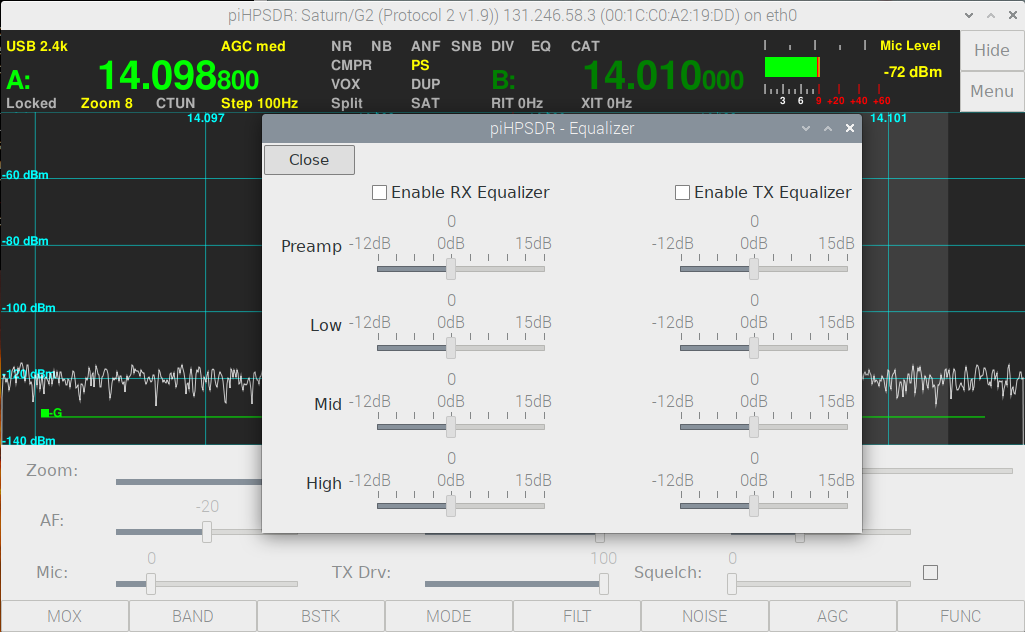
\includegraphics[width=12cm]{EqualizerMenu.png}
\caption{The Equalizer menu}
\label{fig:EqualizerMenu}
\end{figure}

Using \rett{Enable RX Equalizer} and \rett{Enable TX Equalizer},
you can individually enable/disable the RX and TX equalizer.
If the RX equalizer is enabled, the EQ indicator in the
VFO bar, upon receiving, turns yellow and reads \rett{RxEQ}.
If the TX equalizer is enabled, this indicator turns yellow
while transmitting and reads \rett{TxEQ}. So while receiving,
you cannot tell, from the VFO bar, whether the TX equalizer is
actually enabled or not!

For both equalizers, there are four sliders which affect the
overall gain (Preamp), and the amplification in the low/mid/high
frequency range. Equalizer settings are saved with the mode, so
if you adjust the Equaliziers when doing SSB, and then switch to
DIGU, the equalizers are disabled and they resume their SSB
settings upon going back to LSB/USB. This also applies to other
modes such as CWU/CWL, where the TX equalizer has no meaning
anyway, and where the RX equalizer is normally not needed because
CW filters usually are narrow.

For RX-only radios, the TX part of the equalizer menu is not shown.

%%%%%%%%%%%%%%%%%%%%%%%%%%%%%%%%%%%%%%%%%%%%%%%%%%%%%%%%%%%%%%%%%%%%%%%%%%%%%%%%%%%%%%%%%%%%%%%%%%%%%%%%%%%%
\section{The \texttt{Ant} (Antenna) Menu}

The \bltt{Ant} menu, as shown in Fig. \ref{fig:ANTmenu},
applies to HPSDR radios. For SoapySDR radios, the layout
is much simpler because there are much fewer choices possible.

\begin{figure}[ht]
\center
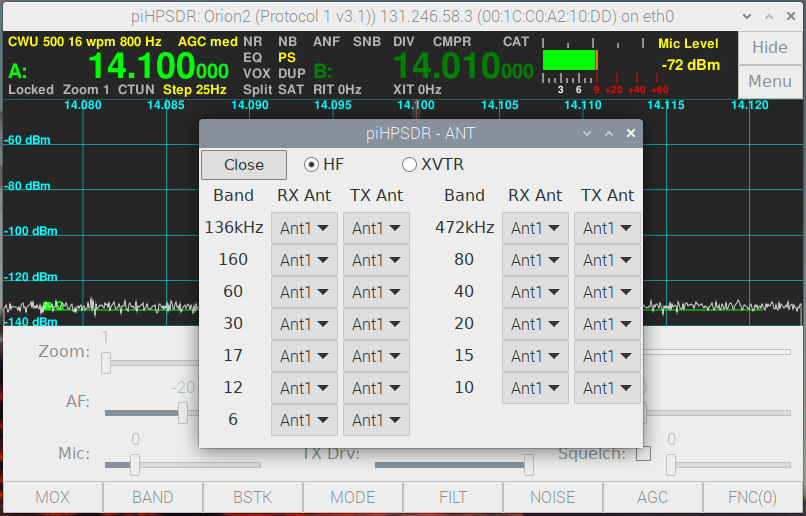
\includegraphics[width=12cm]{ANTmenu.png}
\caption{The ANT (antenna) menu.}
\label{fig:ANTmenu}
\end{figure}

 Standard HPSDR radios have, in most cases, three main antenna jacks
 denoted \rett{Ant1}, \rett{Ant2}, \rett{Ant3}, which can be used both for receiving to
 the first ADC and
 transmitting. Then there are up to additional antenna jacks (\rett{Ext1}, \rett{Ext2},
 and \rett{Xvtr}) which can only be used for receiving and are also connected
 to the first ADC. If the radio has more than one ADC, the (RX only)
 antenna jack, usually denoted RX2, is hard-wired to the second ADC.

 If the menu is opened, the \rett{HF} button is checked, and the HF bands
 are displayed. If one checks the \rett{XVTR} button, the transverter bands
 are shown (this leads to an empty window if no transverter bands have
 yet been defined), and one can go back to the HF bands by re-checking
 \rett{HF}.
 For each band, one can now choose one (out the three) antennas for
 transmitting and one (out of six) antennas for receiving. The main purpose
 of this is the possibility to connect an additional receive-only antenna
such as a beverage antenna which often has a better signal-to-noise
 ration than standard antennas used for transmitting.

\textbf{Transverter operation.} Newer radios (Anan-7000, 8000, and Saturn/G2) have a
switchable low-power TX output. This is enabled if \rett{Xvtr} is selected as the RX antenna of RX1.
The connector used for low-power TX output can also be used for receiving.



%%%%%%%%%%%%%%%%%%%%%%%%%%%%%%%%%%%%%%%%%%%%%%%%%%%%%%%%%%%%%%%%%%%%%%%%%%%%%%%%%%%%%%%%%%%%%%%%%%%%%%%%%%%%
\section{The \texttt{OC} (OpenCollector) Menu}

\begin{figure}[ht]
\center
\includegraphics[width=12cm]{OCMenu.png}
\caption{The OC (open collector) menu.}
\label{fig:OCMenu}
\end{figure}

Standard HPSDR radios have seven individually programmable outputs wired as
open collector output. In the \bltt{OC} menu, you can specify, separately
for each band, and separately for receive and transmit, which output should
be ,,set''. This can be used to switch the band filters of an external PA
or of an external RX preselector, to control an automatic antenna tuner,
and many more things, since it is
your external hardware which in the end has to make sense of the output
bit pattern.

For non-HPSDR radios, the \bltt{OC} menu does not appear in the main menu.

To facilitate control of an automatic tuner, there are seven \rett{TUNE}
bits which are ORed with the bit pattern chosen for TX on the actual band,
as long as you are TUNEing with piHPSDR. Besides the \bltt{TUNE} action,
there are the \bltt{Full TUNE} and \bltt{Memory Tune} actions which are
functionally equivalent, except that the open collector tuning pattern
is removed for \bltt{Full Tune} after the full tune delay, and for \bltt{Memory Tune}
after the memory tune delay, which can also be specified in this menu.
This can be used to send short tuning pulsed of varying length to the
external automatic tuner at the beginning of the tuning.



Note that if you have chosen the \texttt{N2ADR} filter board (see the \bltt{Radio} menu,
this is usually the
case if you are working with a HermesLite-II radio), then the necessary \bltt{OC}
settings for this filter board are enforced upon program start. The same applies if
you enable the \texttt{N2ADR} filter board in the \bltt{Radio} menu.

%%%%%%%%%%%%%%%%%%%%%%%%%%%%%%%%%%%%%%%%%%%%%%%%%%%%%%%%%%%%%%%%%%%%%%%%%%%%%%%%%%%%%%%%%%%%%%%%%%%%%%%%%%%%
%%%%%%%%%%%%%%%%%%%%%%%%%%%%%%%%%%%%%%%%%%%%%%%%%%%%%%%%%%%%%%%%%%%%%%%%%%%%%%%%%%%%%%%%%%%%%%%%%%%%%%%%%%%%
\chapter{The Main Menu: controlling piHPSDR}

In this chapter, the customization of the toolbar (at the bottom of the piHPSDR window),
as well as how to configure GPIO and MIDI controllers, is described. Furthermore, in this
chapter we discuss the RIGCTL menu which allows controlling piHPSDR by some external program
such as a logbook or contest program, via standardized CAT commands that can be sent to
piHPSDR either over a serial line or via TCP.

\textbf{Note for Controller1 owners:} The eight switches (push-buttons) of the controller,
that a positioned below the screen, are bound to the eight toolbar buttons on the screen.
Therefore, there is no "Switches" menu for this controller, and the switches are implicitly
configured via the Toolbar menu.

\begin{figure}[ht]
\center
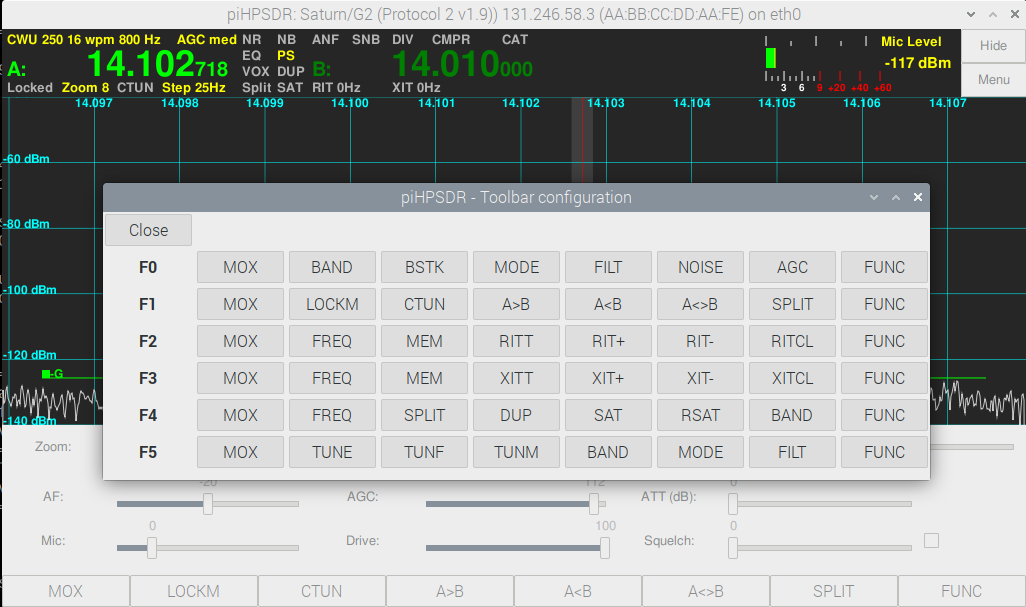
\includegraphics[width=12cm]{ToolbarMenu1.png}
\caption{The Toolbar menu, just opened.}
\label{fig:ToolbarMenu1}
\end{figure}

\section{The \texttt{Toolbar} Menu}
\label{sec:toolbarmenu}
We start with the "Toolbar" menu, that can be found at the top of the rightmost
column in the main menu. The toolbar consists of eight buttons that can be assigned
to a set of eight functions. There are six such sets, and pressing the rightmost button
of the toolbar cycles through these six sets. The text on the rightmost toolbar button, \rett{FNC(0)}, indicates which
layer is currently active.

\begin{figure}[ht!]
\center
\includegraphics[width=12cm]{ToolbarMenu2.png}
\caption{Toolbar menu. Changing second button in \texttt{F1} layer.}
\label{fig:ToolbarMenu2}
\end{figure}

If the \bltt{Toolbar} menu is opened, is looks like Fig. \ref{fig:ToolbarMenu1}.
The rows correspond to the six different layers, and the rightmost button in each
row indicates to which layer this row belongs.
 If one now clicks (just an example)
the \texttt{CTUN} button (third button in the second row) an ,,action dialog'' pops up that looks as
in Fig. \ref{fig:ToolbarMenu2}.


\begin{figure}[ht!]
\center
\includegraphics[width=12cm]{ToolbarMenu3.png}
\caption{Just selected \texttt{Band20}.}
\label{fig:ToolbarMenu3}
\end{figure}

The current action selected (\texttt{CTUN}) is high-lighted. Lists of possible actions can be rather long,
so it might be necessary that you have to scroll up or down in such an action dialog until you have
found what you were looking for. Now (again just an example) the button \texttt{Band 20} has been clicked
in the action dialog, such that it gets high-lighted (Fig. \ref{fig:ToolbarMenu3}).

If one now closes the action dialog by clicking the \texttt{OK} button, the action select menu
closes and on sees that in the toolbar menu now reappearing (Fig. \ref{fig:ToolbarMenu4}), the third button
in the second
line of the toolbar menu has changed, it now gives the short text (\texttt{20}) of the action, which will
switch the active receiver to the 20m band (see the explanation of all the actions in Appendix A).

\begin{figure}[ht!]
\center
\includegraphics[width=12cm]{ToolbarMenu4.png}
\caption{Toolbar assignment accomplished.}
\label{fig:ToolbarMenu4}
\end{figure}

You also see that the toolbar itself has not changed, because we have just changed the \texttt{FNC(1)} set,
while currently the \texttt{FNC(0)} set is active. If one now, however, clicks the rightmost
toolbar button with the text \texttt{FNC(0)} one advances to the next set and the toolbar labels
are updated (Fig. \ref{fig:ToolbarMenu5}).

\begin{figure}[ht!]
\center
\includegraphics[width=12cm]{ToolbarMenu5.png}
\caption{The new \texttt{F1} layer is operative.}
\label{fig:ToolbarMenu5}
\end{figure}

It can be seen that the text of the first seven toolbar buttons has changed to reflect
the functions of the \texttt{F1} set, and also the rightmost button (which is always mapped
to \bltt{Function}) has changed to \texttt{FNC(1)} in oder to indicate the \texttt{F1}
layer is now active. For mouse users (only), a secondary click on the rightmost toolbar
button cycles through the layers in in reverse order.

Note that it is not possible to change the assignment of the  rightmost button of the toolbar,
it will always be assigned to \bltt{Function}, since if one has no access to this
function, one is stuck and can no longer cycle through the function layers.

%%%%%%%%%%%%%%%%%%%%%%%%%%%%%%%%%%%%%%%%%%%%%%%%%%%%%%%%%%%%%%%%%%%%%%%%%%%%%%%%%%%%%%%%%%%%%%%%%%%%%%%%%%%%
\section{The \texttt{RigCtl} (Rig control, or CAT) Menu}

piHPSDR has a built-in rig control or CAT (computer aided transceiver) facility. This can be used to control
piHPSDR from
other programs or even other computers. You can have up to three simultaneous CAT connections via TCP, and
two additional CAT
connections via serial lines (provided the host computer running piHPSDR has those serial interfaces
available). It is
also possible to use FIFOs (also known as named pipes) instead of real serial devices, which offers a
hardware-free connection
of, say, a logbook program running on the same computer to piHPSDR, even if the logbook programm cannot use
TCP. On my Macintosh computer for example, using a named pipe and the Kenwood TS-2000 radio model,
I can connect the MacLogger DX logbook program with piHPSDR.
piHPSDR fully supports (thanks Rick!) the ANDROMEDA controller (see \texttt{github.com/laurencebarker/
Andromeda\_front\_panel}).
This controller (or rather the Arduino inside) is connected to the host computer via USB and appears as a
USB-to-serial
device on the host computer. The CAT command set is explained in Appendix \ref{sec:catcommands}. In most
cases, using
the Kenwood TS-2000 as the radio model would do it, if the digimode or laptop program uses hamlib to
interface with
radios, either choose TS-2000 or (preferably) the ,,OpenHPSDR PiHPSDR'' radio model because this uses time-
out values
adapted to piHPSDR. The \bltt{RigCtl} menu is shown in Fig. \ref{fig:RigCtlMenu}.

\begin{figure}[ht]
\center
\includegraphics[width=12cm]{RigCtlMenu.png}
\caption{The RigCtl (Rig Control) menu.}
\label{fig:RigCtlMenu}
\end{figure}

\rett{RigCtl TCP Port}. This sets the TCP port number for CAT connection to TCP. The default value (19090)
is rather standard,
using another one is only necessary if you are running more than one SDR program on the host computer at the
same time.
This port number must match the port number used in the (digimode or logbook) program that wants to connect.
This value
has no meaning for serial (or named pipe) connections.

\rett{RigCtl Enable}. This checkbock enables or disables the piHPSDR CAT subsystem. Disabling it
automatically also disables
all serial ports.

\rett{Debug}. If enabled, the piHPSDR CAT subsystem sends lots of debug messages to the standard output. If
piHPSDR is run
from within a terminal window, these messages appear in the terminal window. If it is run from double-
clicking a desktop icon,
these messages can be found in a log file within the piHSPDR working directory (this is the directory where
the preferences
are stored. This checkbox is only of interest for software developers to analyze programming or connection
errors, and should
not be checked for normal use.

\rett{Serial Port}. In this text field, enter the device name of the serial port or the named pipe to use.
Which names to use
is highly operating system dependent. On a RaspPi, built-in serial ports have names such as \texttt{/dev/
ttyACM0}. USB-to-serial
adapters (which are nowadays the standard way to add serial ports to a computer) have names such as
\texttt{/dev/ttyUSB0} (on RaspPi) or \texttt{/dev/tty.usbserial-....} (on MacOS). piHPSDR does not try
to ,,detect'' serial
ports, you must know the proper name (e.g. by looking at the contents of the \texttt{/dev} directory).
Named pipes can be created everywhere in the file system hierarchy using the command
,,\texttt{mkdir -p <some\_arbitrary\_name>}''.

To the right of the serial port text field, there is a pop-down menu for choosing the baud rate. Only 4800,
9600, 19200, and 38400 baud are offered, but this should cover most cases. Then, further to the right, is
the \rett{Enable} button which enables a CAT connection on that serial line. Finally, there is the
\rett{Andromeda} check box which should be checked
if that serial port is an ANDROMEDA controller.

If you enable \rett{Andromeda}, the baud rate is automatically set to 9600 baud, and you cannot
change this until you disable \rett{Andromeda}. If you change the baud rate for a serial
port that is already in use (enabled), the serial connection is closed and re-openend
(disabled and enabled).  This also applies
if you enable \rett{Andromeda} for a running serial connection with a baud rate different
from 9600 baud.

The only effect of enabling \rett{Andromeda}, besides fixing the baud rate to 9600 baud,
is that the ANDROMEDA software version is requested (and put into the piHPSDR log file)
once, and that status information is sent over the serial line such that the LEDs of
the ANDROMEDA controller always reflect the current status of piHPSDR.


%%%%%%%%%%%%%%%%%%%%%%%%%%%%%%%%%%%%%%%%%%%%%%%%%%%%%%%%%%%%%%%%%%%%%%%%%%%%%%%%%%%%%%%%%%%%%%%%%%%%%%%%%%%%
\section{The \texttt{MIDI} Menu}
\label{sec:midimenu}
MIDI (musical instrument digital interface) is a protocol designed for the communication of
musical instruments, such as keyboards and tone generators. Because of its widespread use,
support in all major operating systems, and it inherent ability to deliver real-time ,,events'',
it is also an ideal protocol to control an SDR program. The only MIDI messages piHPSDR processes
are NoteOn, NoteOff, and ControllerChange messages. Typically, a NoteOn message is sent if
a key on a keyboard is hit. The first parameter of a NoteOn/Off message is the key
it refers to. Although keyboards rarely have more than 88 keys, the allowed range for
the key is 0-127. There is an additional parameter (,,velocity'', range 0-127) that tells how
fast the key has been hit (this makes the difference between a soft and loud tone on the piano).
NoteOn/Off messages are ideally suited for indicating button press and release events. In principle,
piHPSDR does not need the velocity. However, several MIDI consoles, in a sloppy interpretation of
the MIDI standard, send a NoteOn value with zero velocity if a button is released. Therefore,
piHPSDR interprets a NoteOn message with a velocity different from zero as a ,,button press'',
and interprets both a NoteOn messages with zero velocity and a NoteOff message as a ,,button release''.

The original MIDI standard was built upon a daisy-chained serial connection. Each device
echos all messages it receives at its input side to the output. Therefore, a key-down
message that originated on one keyboard is sent to all tone generators. Likewise, a tone
generator receiving a key-down message cannot tell from which device the message
was originally sent. To resolve possible conflicts, each MIDI message contains a channel
number. There is some confusion about channel numbers: the MIDI says channel numbers
go from 1 to 16. Because this is encoded in a 4-bit data field whose numerical value
goes from 0 to 15, computer users normally refer to channel numbers from 0 to 15,
and this convention is also followed by piHPDSR. Different channel numbers can be used
to discriminate MIDI events from different sources (devices). An example of such a setup
is if you connect a DJ console as well as a microcontroller to which a CW key is attached.

The second type of messages are ControllerChange messages. Typically, they report the value of
an expression pedal, if it has changed. A ControllerChange message also has two parameters,
namely the number of the controller (0-127) and the value (0-127). A ControllerChange
message could be sent if the MIDI controller has a potentiometer, to report its position,
encoded from 0 (full counter clock wise) to 127 (full clock wise). Such a message could then be
used to control in piHPSDR, say, the AF volume or the TX drive. Such a potentiometer is
not suited to become a ,,VFO knob''. Here one uses rotary encoders, a piece of hardware which
you can turn (as long as you like) in either direction, and which reports (by hardware pulses)
how fast and it which direction it is turned. Unfortunately, there is no standard how to
encode these increments into MIDI ControllerChange messages. My Behringer CMD-PL1 console,
for examples, uses ControllerChange numbers 65, 66, 67, $\ldots$ for clockwise rotations
and 63, 62, 61, $\ldots$ for counter clock wise rotations, and further encodes the speed of
rotation in how far the value differs from 64. Other brands interpret the 7-bit number
as a signed quantity, such that values 0, 1, 2, $\ldots$ correspond to clockwise,
and numbers 127, 126, 125, $\ldots$ to counter-clockwise rotations. It is clear that
the piHPSDR MIDI configuration menu must be flexible enough to handle all these situations.

\begin{figure}[ht]
\center
\includegraphics[width=12cm]{MIDImenu1.png}
\caption{The (virgin) MIDI menu.}
\label{fig:MIDImenu1}
\end{figure}

From this it is clear that within piHPSDR, we have to distinguish three types of sources
of MIDI commands:

\rett{KEY}. This type is generated by NoteOn/Off MIDI events. piHPSDR functions (,,Actions'') that
can be assigend to this type are typically those which can also be assigned to toolbar
buttons.

\rett{KNOB/SLIDER}. This type is generaged by ControllerChange MIDI events. It can be used
for piHPSDR functions that are usually controlled by a slider, such as adjusting the AF
volume, setting the TX drive, setting the AGC gain, etc.

\rett{WHEEL}. This type is also generated by ControllerChange MIDI events. This means
that if such an event is configured, the user has to decide whether this event
originated from a potentiometer or from a rotary encoder. The prototypical piHPSDR
function controlled by a WHEEL is a VFO knob, which you can spin forever. However,
you can also assign to to the AF volume control. piHPSDR takes care that the
AF volume stops at the extreme cases (-40 and 0 dB for AF volume) even if you continue
spinning.

The first kind of MIDI device which is often used for SDRs are the so-called MIDI DJ
consoles. If you search the internet for ,,Hercules DJ controller'' or ,,Behringer
DJ controller'' you will find lots of examples. For a very decent price, you
can obtain a device which features lots of controls which you can conveniently use
as VFO knobs, smaller knobs for controlling the AF volume etc., and push buttons
to be used, for example, instead of toolbar buttons. The second kind of MIDI devices
are small MIDI-capable microcontrollers, starting with Teensy and Arduino devices
which have a 32U4 microcontroller which has built-in MIDI capability. With such a
microcontroller, you can build your own "DJ controller". Let the 32U4 control
lots of push buttons and rotary encoders, and send the MIDI messages via USB to the
computer. Using such a micro controller is also the most convenient and general way
to connect a Morse key or paddle to the host computer running piHPSDR (see
Appendix \ref{sec:ConnectCW}, you can but need not use the same micro controller
for taking care of the buttons/encoders and the CW key).

If you open the \bltt{MIDI} menu for the first time, it presents itself as shown
in Fig. \ref{fig:MIDImenu1}.



At the top of the menu, besides the close button, you find a list of MIDI devices
in the system, each of which with a check box. In Fig. \ref{fig:MIDImenu1}, there is only
one such device with name ,,CMD PL-1 MIDI 1''. You will find all MIDI devices attached
to the host computer here. With the check box(es), enable those you want to use.
This way it is possible to run two instances of piHPSDR on the same computer, both
connected to different radios, and control them independently with two different MIDI
consoles. The first thing you have to do is to check all MIDI devices you want to use.

\begin{figure}[ht]
\center
\includegraphics[width=12cm]{MIDImenu2.png}
\caption{The MIDI menu, VFO wheel turned.}
\label{fig:MIDImenu2}
\end{figure}

It is important to note that as long as the MIDI menu is open, piHPSDR cannot be
operated through MIDI. Instead all MIDI messages are captured by the menu and
displayed. This is used to implement a ,,self-learning'' configuration. To explain
this in detail, we demonstrate how to configure MIDI such that the big wheel on the
controller is used as a VFO knob. After I have activated the checkbox of our
MIDI device, I just turned the big wheel of the MIDI console a bit. This resulted
in a menu window that is shown in Fig. \ref{fig:MIDImenu2}. In the third line,
below \rett{Event}, you see \texttt{CTRL} which indicates that the last MIDI messages
received was a ControllerChange message. In the case of a NoteOn/Off messages, this
field would read \texttt{NOTE}. You should rotate the knob in both directions to
see what happens: below \rett{Value} the ControllerChange value of the latest
message is recorded, while the \rett{Min} and \rett{Max} fields report the smallest
and largest value seen (all in the range 0-127). By playing around, it became
quickly clear that this is a rotary encoder, sending messages in the range 65, 66, 67,
$\ldots$ for clockwise rotation and values 63, 62, 61, $\ldots$ for counter clockwise
rotation. If it were a potentiometer, you would see values between 0 and 127
depending on the position of the potentiometer.

Below \rett{Channel}, you see the value zero which
indicates that the channel number of that MIDI message was 1 (see above on the
different channel numberings). Below \rett{Type}, you see a pop-down menu, here
you can choose between \rett{WHEEL} and \rett{Knob/Slider}. In the example shown,
it must be a \rett{WHEEL} since this is a rotary encoder. Because there is no
standard how the values map to increments, a separate panel
\rett{Configure WHEEL parameters} pops up when a wheel is to be configured.
Here one has to define ranges of values that apply for very fast left turns,
fast left turns, normal left turns, normal right turns, fast right turns,
and very fast right turns. Specifying an interval from $-1$ to $-1$ means that
this case will never be realized. In the example shown (Fig. \ref{fig:MIDImenu2}),
we have chosen to map all values from 0-63 to a left turn, and all values from 65-127
to a right turn.
\begin{figure}[ht!]
\center
\includegraphics[width=12cm]{MIDImenu3.png}
\caption{The MIDI menu, selecting VFO action}
\label{fig:MIDImenu3}
\end{figure}

\begin{figure}[ht!]
\center
\includegraphics[width=12cm]{MIDImenu4.png}
\caption{The MIDI menu, VFO action selected}
\label{fig:MIDImenu4}
\end{figure}
Now we have to specify which piHPSDR function should be triggered when moving the wheel.
The current action is shown in a button below the string \rett{Action} and defaults to \bltt{NONE}.
By clicking this button, a dialog to choose the function opens as described for the
\bltt{Toolbar} menu (chapter \ref{sec:toolbarmenu}), with the current choice (\bltt{NONE})
highlighted. The only difference is that now only functions are listed that can be
assigned to encoders.
Because we want to assign the wheel to the \bltt{VFO} function, we click
the \bltt{VFO} button, which then becomes highlighted (Fig. \ref{fig:MIDImenu3}).



 Then one has to click the OK button to make the choice, and one returns to the
 MIDI menu (see Fig. \ref{fig:MIDImenu4}).

One sees that the choise has entered the MIDI configuration, as documented by the
list in the bottom right part of the menu. At this stage, we can continue
assigning more encoders, potentiometers, or buttons. If we close the menu at
this point, then the big wheel on the MIDI console can immediately be used
to change the VFO frequency.

%%%%%%%%%%%%%%%%%%%%%%%%%%%%%%%%%%%%%%%%%%%%%%%%%%%%%%%%%%%%%%%%%%%%%%%%%%%%%%%%%%%%%%%%%%%%%%%%%%%%%%%%%%%%
\section{The \texttt{Encoders} Menu}
\begin{figure}[ht!]
\center
\includegraphics[width=12cm]{g2_frontpanel.png}
\caption{A picture of the G2 frontpanel (image courtesy of Apache Labs).}
\label{fig:g2_frontpanel}
\end{figure}

\begin{figure}[ht]
\center
\includegraphics[width=12cm]{EncoderMenuG2.png}
\caption{The Encoder menu for the G2 frontpanel controller}
\label{fig:EncoderMenuG2}
\end{figure}
The encoders menu can be used to assign functions to the encoders of a
piHPSDR Controller1, Controller2 or the G2 front panel controller.
If \texttt{No Controller} has been chosen in the initial discovery screen
(Fig. \ref{fig:Start}), this menu is not available.
Note that the ,,large knob'' of these controllers
cannot be assigned a function, it is hard-wired to the \bltt{VFO} function.



While the function of this menu is the same in all three cases (Controller1, Controller2,
G2 frontpanel), the layout is different, because the position of the menu buttons
are meant to indicate which encoder is referred to.



The G2 frontpanel (Fig. \ref{fig:g2_frontpanel}) has,
in addition to the large VFO knob at the bottom right,
four small knobs, two (one above the other)
at the left edge and two at the right edge. All four knobs are double encoders with
a switch. This means that there is an inner/upper knob (,,top encoder'')
and an outer/lower knob (,,bottom encoder''), which
are two separate encoders. Furthermore, you can push the knob and have and additional
push button function (,,Switch''). If you open the \bltt{Encoders} menu for
a G2 frontpanel controller, the menu opens as shown in Fig. \ref{fig:EncoderMenuG2}.
You see four groups with three buttons (Switch, Top, Bottom) each, and it should be
clear which group belongs to which encoder. With the buttons, you can choose which function
to assign, in the same way as described for the \bltt{Toolbar} (chapter \ref{sec:toolbarmenu})
and \bltt{MIDI} (chapter \ref{sec:midimenu}) menus. With the \rett{Default} button, you can
re-assign the default values (those shown in Fig. \ref{fig:EncoderMenuG2})
to the encoder functions, which match the silk printing
on the enclosure (see Fig. \ref{fig:g2_frontpanel}).

\begin{figure}[ht!]
\center
\includegraphics[width=12cm]{Apache_Controller2.png}
\caption{A picture of the Controller2 (image by courtesy of Apache Labs).}
\label{fig:Apache_Controller2}
\end{figure}

The Controller2 (see Fig. \ref{fig:Apache_Controller2}
has (besides the VFO knob at the bottom right) three knobs (arranged horizontally) at the bottom left,
and a fourth knob at the top right, all of which are double encoders with a switch.
So if you run piHPSDR with a Controller2, then the menu looks different (Fig. \ref{fig:EncoderMenuV2}).
 The menu shows
for groups with three buttons each, and it should be clear which group belongs to which button. The
\rett{Default} button again re-installs the default functions (those shown in Fig. \ref{fig:EncoderMenuV2}).

\begin{figure}[ht!]
\center
\includegraphics[width=12cm]{EncoderMenuV2.png}
\caption{The Encoder menu for Controller2}
\label{fig:EncoderMenuV2}
\end{figure}

\begin{figure}[ht!]
\center
\includegraphics[width=12cm]{Apache_Controller1.png}
\caption{A picture of the Controller1 (image by courtesy of Apache Labs).}
\label{fig:Apache_Controller1}
\end{figure}


Finally, the Controller1 (see Fig. \ref{fig:Apache_Controller1})
has (besides the big VFO knob at the bottom right)
three knobs (denoted E1, E2, E3), rranged vertically at the right edge. These knobs
are single encoders with a switch (you can turn the knob, but you can also push it). Therefore,
the \bltt{Encoders} menu in this case (Fig. \ref{fig:EncoderMenuV1}) shows three groups with
two buttons each. The \rett{Default} button again re-installs the default values shown in
Fig. \ref{fig:EncoderMenuV1}, these are chosen just for convenience since there are no default
function printed on the enclosure.

\begin{figure}[ht!]
\center
\includegraphics[width=12cm]{EncoderMenuV1.png}
\caption{The Encoder menu for Controller1}
\label{fig:EncoderMenuV1}
\end{figure}

%%%%%%%%%%%%%%%%%%%%%%%%%%%%%%%%%%%%%%%%%%%%%%%%%%%%%%%%%%%%%%%%%%%%%%%%%%%%%%%%%%%%%%%%%%%%%%%%%%%%%%%%%%%%
\section{The \texttt{Switches} Menu}

The encoders menu can be used to assign functions to the push buttons of a
piHPSDR  Controller2 or the G2 front panel controller.
If \texttt{No Controller} or \texttt{Controller1} has been chosen in the initial discovery screen
(Fig. \ref{fig:Start}), this menu is not available. This menu is not available
for the Controller1 because the eight push buttons of this controller are hard-wired to
the toolbar buttons and their functions as thus assigned via the \bltt{Toolbar} menu
(see Chapter \ref{sec:toolbarmenu}).

On the G2 frontpanel (see Fig. \ref{fig:g2_frontpanel}),
 there are a lot of push buttons: at the left edge, to the right
of the left edge encoders, are two buttons, at the bottom right, below the VFO knob,
there are two more buttons, and at the top right, to the right of the left edge
encoders, is an array of 12 (4x3) buttons. The layout of the \bltt{Switches} menu
for the G2 frontpanel (Fig. \ref{fig:SwitchMenuG2}) features (besides the Close
button) sixteen buttons, and their arrangement is such that you can easily guess
which menu button refers to which button on your G2 frontpanel. Assigning functions
to these buttons is done exactly as described for the \bltt{Toolbar} menu
(chapter \ref{sec:toolbarmenu}). With \rett{Default} one re-installs the default values
shown in Fig. \ref{fig:SwitchMenuG2} which match the functions printed on the enclosure.

\begin{figure}[ht]
\center
\includegraphics[width=12cm]{SwitchMenuG2.png}
\caption{The Switches menu for the G2 frontpanel controller.}
\label{fig:SwitchMenuG2}
\end{figure}

The Controller2 (see Fig. \ref{fig:Apache_Controller2} in the last section)
also has 16 push buttons, but they are arranged differently:
at the bottom edge there are 7 buttons arranged horizontally. At the right
edge, there is an array of 8 buttons (4x2) with one additional button
above the right column that is to the right of the fourth encoder, just
below the power button. Looking at the \bltt{Switches} menu for the
Controller2 (Fig. \ref{fig:SwitchMenuV2}), you see representations of
these 16 buttons in an arrangement for which it is self evident which
menu button refers to which Controller2 push button.
Assigning functions
to these buttons is done exactly as described for the \bltt{Toolbar} menu
(chapter \ref{sec:toolbarmenu}).
With \rett{Default} one re-installs the default values
shown in Fig. \ref{fig:SwitchMenuV2} which match the functions printed on the enclosure.

\begin{figure}[ht]
\center
\includegraphics[width=12cm]{SwitchMenuV2.png}
\caption{The Switches menu for Controller2.}
\label{fig:SwitchMenuV2}
\end{figure}


\appendix
%%%%%%%%%%%%%%%%%%%%%%%%%%%%%%%%%%%%%%%%%%%%%%%%%%%%%%%%%%%%%%%%%%%%%%%%%%%%%%%%%%%%%%%%%%%%%%%%%%%%%%%%%%%%
%%%%%%%%%%%%%%%%%%%%%%%%%%%%%%%%%%%%%%%%%%%%%%%%%%%%%%%%%%%%%%%%%%%%%%%%%%%%%%%%%%%%%%%%%%%%%%%%%%%%%%%%%%%%
\chapter{List of piHPSDR ,,Actions''}
\label{sec:actionlist}

In this chapter, we give a list of ,,actions'' implemented in the piHPSDR program. These actions can be
assigned to toolbar buttons on the screen, or pushbuttons/encoders of a GPIO-connected or MIDI controller.
Not all actions can be assigned to all control elements. Changing the AF volume, for example, can only be
assigned to a knob
which you can turn, while switching RIT on/off can only be assigned to a button that you can push. For each
action in the following table, there is a long and a short string assigned. The long string will be used
when there is enough space, while the short string is used for small buttons and to store actions in
preference files (therefore the short strings never contain a blank character or a line break). Then, for
each action we give the type of control element allowed for this action as a combination of the letters B,
P, E, which stand for

\begin{itemize}[font=\texttt, left=0pt]
\item[B] {"Button": A button in the toolbar, or a push-button or switch on a GPIO or MIDI connected console}
\item[P] {"Potentiometer": A potentiometer or a slider on a MIDI connected console}
\item[E] {"Encoder": A rotary encoder on a GPIO or MIDI connected console}
\end{itemize}

The main difference between a "potentiometer" and an "encoder" is, that the former has a min and max
position, while
an encoder can be turned in either direction without stopping. This means that a potentiometer
reports a value between min and max, while an encoder reports an increment,
that is, whether it has been turned clock wise or counter clock wise.
The existing GPIO consoles do not have potentiometers (most likely because of the lack of analog inputs),
but
many MIDI consoles do have, and Arduino-based MIDI controllers might have it because there analog inputs
to read out potentiometers are available.

To give an example, controlling the TX drive can be down both with a slider and with an encoder. While for
a slider/potentiometer, the values from min to max are simple mapped to the TX drive values from 0 to 100,
the signals from an encoder will just increase or decrease the value until one of a limits has been reached.

In the following, the actions are alphabetically sorted by their long name, with the "empty" action listed
first.

\renewcommand{\belowrulesep}{0pt}
\renewcommand{\aboverulesep}{0pt}
\def\action#1#2#3#4{
\begin{center}
\begin{tabular}{|p{7cm}|p{3cm}|p{1cm}|}
\toprule
$\phantom{\Big|}$\bltt{\large #1} & \texttt{\large #2} & \texttt{\large #3} \\\cline{1-3}
\multicolumn{3}{|p{\textwidth}|}{#4} \\
\bottomrule
\end{tabular}
\end{center}
}


\action{NONE}{NONE}{BPE}{This is an action which does nothing. It can be assigned to buttons or enco\-ders
that
are often accidentally operated. Some MIDI consoles, for example, report a button press event if the VFO
knob is touched, and this we want to ignore.}

\action{A<>B}{A<>B}{B}{Swap VFOs A and B. This will not only swap the frequencies, but also all other
settings
associated with that VFO, such as mode, filter, CTUN, and RIT settings.}

\action{A<B}{A<B}{B}{Copy VFO B to VFO A.}

\action{A>B}{A>B}{B}{Copy VFO A to VFO B.}

\action{AF Gain}{AFGAIN}{PE}{Change the AF gain (headphone volume) of the active receiver.}

\action{AF Gain RX1}{AFGAIN1}{PE}{Change the AF gain (headphone volume) of the RX1 receiver.}

\action{AF Gain RX2}{AFGAIN2}{PE}{Change the AF gain (headphone volume) of the RX2 receiver.}

\action{AGC Menu}{AGC}{B}{Opens the \texttt{AGC} menu.}

\action{ANF}{ANF}{B}{Toggels the state (on/off) of the automatic notch filter for the active receiver.}

\action{Atten}{ATTEN}{PE}{Changes the value (0-31 dB) of the step attenuator of the active receiver.
This funciton is only available for radios that have such an attenuator.}

\action{Band 10}{10}{B}
{Change band of the active receiver to the 10m band. If already on that band, move to
the next bandstack entry. This action is a no-op if the frequency of the band falls outside the frequency
range of the radio.}

\action{Band 12}{12}{B}
{Change band of the active receiver to the 12m band. If already on that band, move to
the next bandstack entry. This action is a no-op if the frequency of the band falls outside the frequency range
of the radio.}

\action{Band 1240}{1240}{B}
{Change band of the active receiver to the 1240 MHz (23 cm) band. If already on that band, move to
the next bandstack entry. This action is a no-op if the frequency of the band falls outside the frequency
range of the radio.}

\action{Band 144}{144}{B}
{Change band of the active receiver to the 144 MHz (2m) band. If already on that band, move to
the next bandstack entry. This action is a no-op if the frequency of the band falls outside the frequency
range of the radio.}

\action{Band 15}{15}{B}
{Change band of the active receiver to the 15m band. If already on that band, move to
the next bandstack entry. This action is a no-op if the frequency of the band falls outside the frequency
range of the radio.}

\action{Band 160}{160}{B}
{Change band of the active receiver to the 160m band. If already on that band, move to
the next bandstack entry. This action is a no-op if the frequency of the band falls outside the frequency
range of the radio.}

\action{Band 17}{17}{B}
{Change band of the active receiver to the 15m band. If already on that band, move to
the next bandstack entry. This action is a no-op if the frequency of the band falls outside the frequency
range of the radio.}

\action{Band 20}{20}{B}
{Change band of the active receiver to the 15m band. If already on that band, move to
the next bandstack entry. This action is a no-op if the frequency of the band falls outside the frequency
range of the radio.}

\action{Band 220}{220}{B}
{Change band of the active receiver to the 220 MHz (1.25 m) band. If already on that band, move to
the next bandstack entry. This action is a no-op if the frequency of the band falls outside the frequency
range of the radio.}

\action{Band 2300}{2300}{B}
{Change band of the active receiver to the 2300MHz (13 cm) band. If already on that band, move to
the next bandstack entry. This action is a no-op if the frequency of the band falls outside the frequency
range of the radio.}

\action{Band 30}{30}{B}
{Change band of the active receiver to the 30m band. If already on that band, move to
the next bandstack entry. This action is a no-op if the frequency of the band falls outside the frequency
range of the radio.}

\action{Band 3400}{3400}{B}
{Change band of the active receiver to the 3400 Mhz (9 cm) band. If already on that band, move to
the next bandstack entry. This action is a no-op if the frequency of the band falls outside the frequency
range of the radio.}

\action{Band 40}{40}{B}
{Change band of the active receiver to the 40m band. If already on that band, move to
the next bandstack entry. This action is a no-op if the frequency of the band falls outside the frequency
range of the radio.}

\action{Band 430}{430}{B}
{Change band of the active receiver to the 430 MHz (70 cm) band. If already on that band, move to
the next bandstack entry. This action is a no-op if the frequency of the band falls outside the frequency
range of the radio.}

\action{Band 6}{6}{B}
{Change band of the active receiver to the 6m band. If already on that band, move to
the next bandstack entry. This action is a no-op if the frequency of the band falls outside the frequency
range of the radio.}

\action{Band 60}{60}{B}
{Change band of the active receiver to the 60m band. If already on that band, move to
the next bandstack entry. This action is a no-op if the frequency of the band falls outside the frequency
range of the radio.}

\action{Band 70}{70}{B}
{Change band of the active receiver to the 70 MHz (4m)  band. If already on that band, move to
the next bandstack entry. This action is a no-op if the frequency of the band falls outside the frequency
range of the radio.}

\action{Band 80}{80}{B}
{Change band of the active receiver to the 80m band. If already on that band, move to
the next bandstack entry. This action is a no-op if the frequency of the band falls outside the frequency
range of the radio.}

\action{Band 902}{902}{B}
{Change band of the active receiver to the 902 MHz (33 cm) band. If already on that band, move to
the next bandstack entry. This action is a no-op if the frequency of the band falls outside the frequency
range of the radio.}

\action{Band AIR}{AIR}{B}
{Change band of the active receiver to the 108 MHz band, used for aircraft communication. If already on that
band, move to
the next bandstack entry. This action is a no-op if the frequency of the band falls outside the frequency
range of the radio.}

\action{Band GEN}{GEN}{B}
{Change band of the active receiver to the current bandstack entry of the "general" band. If already on that
band, move to
the next bandstack entry. This action is a no-op if the frequency of the band falls outside the frequency
range of the radio.}

\action{Band -}{BND-}{B}
{Change band of the active receiver to the next lower band in the list of bands. If already at the lowest
band, switch to the highest band (including transverter bands which have been defined) whose frequency is
with the radio's frequency range.}

\action{Band +}{BND+}{B}
{Change band of the active receiver to the next higher band in the list of bands (including transverter
bands that have been defined). If already at the highest band, switch to the lowest band whose frequency is
with the radio's frequency range.}

\action{Band WWV}{WWV}{B}
{Change band of the active receiver to the current bandstack entry of the WWV band. If already on that band,
move to the next bandstack entry. This action is a no-op if the frequency of the band falls outside the
frequency range of the radio.}

\action{BndStack -}{BSTK-}{B}
{Cylcle backward through the bandstack entries of the active receiver.}

\action{BndStack +}{BSTK+}{B}
{Cylcle forward through the bandstack entries of the active receiver.}

\action{Band Menu}{BAND}{B}
{Open the \texttt{BAND} menu.}

\action{BndStack MENU}{BSTK}{B}
{Open the \texttt{BANDSTACK} menu.}

\action{Cmpr On/Off}{COMP}{B}
{Toggle the state (on/off) of the compressor used in the TX audio input.}

\action{Cmpr Level}{COMPVAL}{PE}
{Change the value of the compressor (0-20 dB) used in the TX audio input. The compressor is automaticall
switched on (off) if the "new" value of the compressor is larger then  (equal to) zero.}

\action{CTUN}{CTUN}{B}
{Toggle the state (on/off) of the CTUN state of the active receiver. CTUN stands for "click to tune". In
CTUN mode, you can move
the RX frequency over the whole spectrum scope, whose center then remains at a fixed frequency.}

\action{CW Audio Peak Fltr}{CW-APF}{B}
{Toggle (on/off) the CW audio peak filter for the active receiver. Note that the width of this
filter (default: 75 Hz) can only be modified through the \bltt{CW} menu.}

\action{CW Frequency}{CWFREQ}{PE}
{Change the CW side tone frequency in the range 300-1000 Hz. This also changes the BFO frequency upon
receive.}

\action{CW Left}{CWL}{B}
{This action indicates the closure/opening of the left paddle of a CW key. It is usually assigned to a GPIO
line or a MIDI
controller to which a Morse paddle is attached, and works with the iambic keyer that is built into piHPSDR.
This keyer
is only active if CW is \textit{not} handled in the radio (see CW menu).}

\action{CW Right}{CWR}{B}
{This action indicates the closure/opening of the right paddle of a CW key. It is usually assigned to a GPIO
line or a MIDI
controller to which a Morse paddle is attached, and works with the iambic keyer that is built into piHPSDR.
This keyer
is only active if CW is \textit{not} handled in the radio (see CW menu).}

\action{CW Speed}{CWSPD}{PE}
{Change the CW side tone frequency in the range 1-60 wpm. This affect the built-in iambic keyer or the keyer
inside the radio,
depending on whether CW is handled in the radio or not (see CW menu).}

\action{CW Key (keyer)}{CWKy}{B}{Straith key key-down or key-up event. Usually assigned to a GPIO line of
MIDI controller to
which a straight key or an external keyer is attached. Note that this action does not automatically switch
to TX, so it must
be used together with either manual RX/TX switching, or with the "\texttt{PTT (CW Keyer)}" action.}

\action{PTT (keyer)}{CWKyPTT}{B}{This very similar to the \texttt{PTT} action (see below) with the exception
that CW handling in the radio is temporarily disabled (thus, CW handling in piHPSDR is enabled). This allows
to have, e.g. a paddle attached
to the radio while a contest logging program ,,talks'' to piHPSDR.}

\action{DIV On/Off}{DIVT}{B}{Toggles (enabled/disabled) DIVERSITY reception.}

\action{DIV Gain}{DIVG}{E}{Adjust DIVERSITY gain. One tick of the encoder increments of decrements the gain
by an amount of 0.5}

\action{DIV Gain Coarse}{DIVGC}{E}{Adjust DIVERSITY gain (coarse adjustment).  One tick of the encoder
increments of decrements the gain by an amount of 2.5}

\action{DIV Gain Fine}{DIVGF}{E}{Adjust DIVERSITY gain (fine adjustment).  One tick of the encoder
increments of decrements the gain by an amount of 0.1.
Since adjusting the DIVERSITY gain (or phase) is sometimes difficult, assigning one encoder to a coarse and
another encoder to a fine adjustment may
help in locating the ,,sweet spot''.}

\action{DIV Phase}{DIVP}{E}{Adjust DIVERSITY phase (fine adjustment). One tick of the encoder increments of
decrements the gain by an amount of 0.5}

\action{DIV Phase Coarse}{DIVPC}{E}{Adjust DIVERSITY gain (coarse adjustment). One tick of the encoder
increments of decrements the gain by an amount of 2.5}

\action{DIV Phase Fine}{DIVPF}{E}{Adjust DIVERSITY gain (coarse adjustment). One tick of the encoder
increments of decrements the gain by an amount of 20.1}

\action{DIV Menu}{DIV}{B}{Open the DIVERSITY menu.}

\action{Duplex}{DUP}{B}{Toggle (on/off) DUPLEX status. IN the DUPLEX mode, the receivers continue to work
during TX, and the RX panels are not
removed during TX. Instead, a separate TX window opens during transmitting. Generally, DUPLEX only make
sense when using different and well
decoupled RX and TX antennas.}

\action{Filter -}{FL-}{B}{Cycle forward (!) through the list of filters for the current mode of the active
receiver. Normally, this means switching
to a narrower filter (hence the name \texttt{FILTER -}). When reaching the last filter in the list, further
cycling switches to the first
(widest) filter.}

 \action{Filter +}{FL+}{B}{Cycle backward (!) through the list of filters for the current mode of the active
receiver. Normally, this means switching
to a wider filter (hence the name \texttt{FILTER +}). When reaching the first filter in the list, further
cycling switches to the last
filter which is the variable \texttt{Var2} filter.}

\action{Filter Cut Low}{FCUTL}{E}{Adjust the low-cut of the current filter. Note that the notion of ,,low''
edge of the filter refers to
audio frequencies for the single side band modes LSB, CWL, DIGL. This action is a no-op unless the current
filter is one of the two variable filters
 \texttt{Var1} or \texttt{Var2}.}

\action{Filter Cut High}{FCUTL}{E}{Adjust the high-cut of the current filter. Note that the notion
of ,,high'' edge of the filter refers to
audio frequencies for the single side band modes LSB, CWL, DIGL. This action is a no-op unless the current
filter is one of the two variable filters
 \texttt{Var1} or \texttt{Var2}.}

 \action{Filter Cut Default}{FCUTDEF}{B}{Reset the low and high cut of the current filter to the default
 values. This action is a no-op unless the current filter is one of the two variable filters
 \texttt{Var1} or \texttt{Var2}.}

 \action{Filter Menu}{FILT}{B}{This opens the \texttt{Filter} menu.}

 \action{VFO Menu}{FREQ}{B}{This opens the \texttt{FREQ} (VFO) menu.}

 \action{Function}{FUNC}{B}{Cycle through the six toolbar sets. For the piHPSDR GPIO Controller1, where
 the eight switches follow the toolbar buttons, this also affects the function
 of the switches. Note that this action is \textit{always} connected with the right-most toolbar button.}

  \action{FuncRev}{FUNC-}{B}{Cycle backwards through the six toolbar sets. For the piHPSDR GPIO Controller1,
   where the eight switches follow the toolbar buttons, this also affects the function
 of the switches. When using a mouse, this action can be invoked by a secondary mouse click
 on the rightmost toolbar button.}

 \action{IF Shift}{IFSHFT}{E}{This command is effective only if one of the variable filters Var1 or Var2 is
 currently used in the  active receiver, and shifts the  filter, that is,
 it affects  the low and high cut in the same way.}

 \action{IF Shift RX1}{IFSHFT1}{E}{This command is effective only if one of the variable filters Var1 or
 Var2 is currently used in VFO-A, and shifts the filter, that is,
 it affects  the low and high cut in the same way.}

 \action{IF Shift RX2}{IFSHFT2}{E}{This command is effective only if one of the variable filters Var1 or
 Var2 is currently used in VFO-B, and shifts the filter, that is,
 it affects  the low and high cut in the same way.}

 \action{IF Width}{IFWIDTH}{E}{This command is effective only if one of the variable filters Var1 or Var2 is
 currently used in the  active receiver, and changes the  filter width, that is,
 it affects  the low and high cut in an opposite way.}

 \action{IF Width RX1}{IFWIDTH1}{E}{This command is effective only if one of the variable filters Var1 or
 Var2 is currently used in VFO-A, and changes the  filter width, that is,
 it affects  the low and high cut in an opposite way.}

 action{IF Width RX2}{IFWIDTH2}{E}{This command is effective only if one of the variable filters Var1 or
 Var2 is currently used in VFO-B, and changes the  filter width, that is,
 it affects  the low and high cut in an opposite way.}

\action{Linein Gain}{LIGAIN}{PE}{Change the line-in gain of the radio. If the
     radio does not have a line-in input, this control has no effect.}

\action{Lock}{LOCK}{B}{Lock the VFOs. A locked VFO will not accept VFO frequency steps in either direction,
and cannot be moved by dragging with the  mouse. Band changes etc.
are still possible, though. The command is intended to guard against accidentally moving the VFO dial.}

\action{Memory Menu}{MEM}{B}{Open the \texttt{MEM} (Memory) menu.}

\action{Mic Gain}{MICGAIN}{PE}{Change the mic gain (from -12 to 50 dB). The amplification of the microphone
audio data is done in software, and applies to the TX audio
input samples whereever they come from. (See the discussion of local microphones in the \texttt{TX} menu.}

\action{Mode -}{MD-}{B}{Cycle backwards through the list of modes for the active receiver. When the first
mode (LSB) has been reached, jump to the last one (DRM). Note that when
changing the mode, the current filter, noise reduction, equalizer, VFO step size, and TX compressor settings
are stored for the old mode, and the settings last used with the
new mode are restored. This allows to quickly switch between SSB and CW, or between SSB and digi modes,
without re-adjusting these settings.}

\action{Mode +}{MD+}{B}{Cycle forward through the list of modes for the active receiver. When the last mode
(DRM) has been reached, jump to the first one (LSB). Note that when
changing the mode, the current filter, noise reduction, equalizer, VFO step size, and TX compressor settings
are stored for the old mode, and the settings last used with the
new mode are restored. This allows to quickly switch between SSB and CW, or between SSB and digi modes,
without re-adjusting these settings.}

\action{Mode Menu}{MODE}{B}{Open the \bltt{Mode} menu.}

\action{MOX}{MOX}{B}{Toggle between TX and RX. Unlike the PTT action, which puts the radio into TX when
pressed and into RX when released, this button toggles the PTT state
when pressed.}

\action{Mute}{MUTE}{B}{Toggles the ,,mute'' state of the active receiver. If a receiver is muted, it
produces zero-amplitude audio output.}

\action{NB}{NB}{B}{Cycles through the noise blanker states (NB off/NB1/NB2).}

\action{NR}{NR}{B}{Cycles through the noise reduction states (NR off/NR1/NR2).}

\action{Noise Menu}{NOISE}{B}{Opens the \texttt{NOISE} menu.}

\action{NumPad 0}{0}{B}{Used for direct frequency entry. This is the same as hitting the corresponding
button ,,0'' in the \texttt{VFO} (VFO) menu.}

\action{NumPad 1}{1}{B}{Used for direct frequency entry. This is the same as hitting the corresponding
button ,,1'' in the \texttt{VFO} menu.}

\action{NumPad 2}{2}{B}{Used for direct frequency entry. This is the same as hitting the corresponding
button ,,2'' in the \texttt{VFO} menu.}

\action{NumPad 3}{3}{B}{Used for direct frequency entry. This is the same as hitting the corresponding
button ,,3'' in the \texttt{VFO} menu.}

\action{NumPad 4}{4}{B}{Used for direct frequency entry. This is the same as hitting the corresponding
button ,,4'' in the \texttt{VFO} menu.}

\action{NumPad 5}{5}{B}{Used for direct frequency entry. This is the same as hitting the corresponding
button ,,5'' in the \texttt{VFO} menu.}

\action{NumPad 6}{6}{B}{Used for direct frequency entry. This is the same as hitting the corresponding
button ,,6'' in the \texttt{VFO} menu.}

\action{NumPad 7}{7}{B}{Used for direct frequency entry. This is the same as hitting the corresponding
button ,,7'' in the \texttt{VFO} menu.}

\action{NumPad 8}{8}{B}{(Used for direct frequency entry. This is the same as hitting the corresponding
button ,,8'' in the \texttt{VFO}  menu.}

\action{NumPad 9}{9}{B}{Used for direct frequency entry. This is the same as hitting the corresponding
button ,,9'' in the \texttt{VFO}  menu.}

\action{NumPad BS}{BS}{B}{Used for direct frequency entry (BS = backstep). This is the same as hitting the
corresponding button  in the \texttt{VFO} menu. It cancels the last-entered digit.}

\action{NumPad CL}{CL}{B}{Used for direct frequency entry (CL = clear). This is the same as hitting the
corresponding button  in the \texttt{VFO}  menu. It cancels all entered digits so far.}

\action{NumPad Dec}{DEC}{B}{Used for direct frequency entry (DEC = decimal point). This is the same as
hitting the corresponding button  in the \texttt{VFO} menu.}

\action{NumPad kHz}{KHZ}{B}{Used for direct frequency entry. This is the same as hitting the corresponding
button  in the \texttt{VFO}  menu. The VFO frequency is changed to the value entered so far, multiplied with
1000. For example, to go to 7.040 MHz, one can enter the sequence ,,7'', ,,0'', ,,4'', ,,0'', ,,KHZ''.}

\action{NumPad MHz}{MHZ}{B}{Used for direct frequency entry. This is the same as hitting the corresponding
button
in the \texttt{VFO}  menu. The VFO frequency is changed to the value entered so far, multiplied with
1,000,000.
For example, to go to 7.040 MHz, one can enter the sequence ,,7'', ,,DEC'', ,,0'', ,,4'', ,,MHZ''.}

\action{NumPad Enter}{EN}{B}{Used for direct frequency entry. This is the same as hitting the corresponding
button  in the \texttt{VFO}  menu. The VFO frequency is changed to the value entered so far.
For example, to go to 7.040 MHz, one can enter the
sequence ,,7'',  ,,0'', ,,4'', ,,0'', ,,0'', ,,0'', ,,0''. This
is rarely used but offers Hz-resolution for the direct frequency entry.}

\action{PanZoom}{PAN}{E}{Change the Pan value. This control is only effective when the Zoom value is larger
than 1.}

\action{Pan-}{PAN-}{B}{Decrease the PAN value by 100. This control is only effective when the Zoom value is
larger than 1.}

\action{Pan+}{PAN+}{B}{Increase the PAN value by 100. This control is only effective when the Zoom value is
larger than 1.}

\action{Panadapter High}{PANH}{PE}{Change the dBm value (from -60 to +20) at the top of the spectrum scope
of the active receiver. Values outside
this range can be set in the \texttt{DISPLAY} menu.}

\action{Panadapter Low}{PANL}{PE}{Change the dBm value (from -160 to -60) at the bottom of the spectrum
scope of the active receiver.
Values outside this range can be set in the \texttt{DISPLAY} menu.}

\action{Panadapter Step}{PANS}{PE}{Change the step size (from 5 to 30) of the panadapter of the active
receiver. This is the spacing
of the thin horizontal  lines in the spectrum scope.}

\action{Preamp On/Off}{PRE}{B}{Toggle the preamp of the active receiver. Although the preamp switching is
part of the HPSDR protocol,
this has no effect in current radio models since the preamp is hard-wired ,,on''.}

\action{PS On/Off}{PST}{B}{Toggle (on/off) adaptive predistortion (PureSignal).}

\action{PS Menu}{PS}{B}{Open the \texttt{PS} (PureSignal) menu.}

\action{PTT}{PTT}{B}{Put the radio  into TX mode when the button is pressed, and go back to RX when the
button is released. This is
one of the few actions where a button release event is significant. When attaching, say, the PTT contact of
a microphone to
a GPIO line for this purpose, take care of proper debouncine, since piHPSDR is not good at debouncing
switches where both
the press and release events are significant.}

\action{RF Gain}{RFGAIN}{PE}{Set the gain of the RF front end of the active receiver. Only effective for
radios that have such a
gain control. Most HPSDR radios do not have RF  gain, they have a step attenuator in the RF front end
instead. Small SDR radios
using the AD9866 chip (HermesLite, RadioBerry) and radios connected via the SoapySDR library usually do have
an RF gain control.}

\action{RF Gain RX1}{RFGAIN1}{PE}{Set the gain of the RF front end of RX1. Only effective for radios that
have such a
gain control. Most HPSDR radios do not have RF  gain, they have a step attenuator in the RF front end
instead. Small SDR radios
using the AD9866 chip (HermesLite, RadioBerry) and radios connected via the SoapySDR library usually do have
an RF gain control.}

\action{RF Gain RX2}{RFGAIN2}{PE}{Set the gain of the RF front end of RX2. Only effective for radios that
have such a
gain control. Most HPSDR radios do not have RF  gain, they have a step attenuator in the RF front end
instead. Small SDR radios
using the AD9866 chip (HermesLite, RadioBerry) and radios connected via the SoapySDR library usually do have
an RF gain control.}

\action{RIT}{RIT}{E}{Change the RIT value of the active receiver in the range -9999 to 9999 Hz. If a zero
value is set, RIT is
automatically disabled, if a non-zero value ist set, RIT is enabled.}

\action{RIT Clear}{RITCL}{B}{Set the RIT value of the active receiver to zero. As a side effect, RIT is
disabled for the active receiver}

\action{RIT On/Off}{RITT}{B}{Toggle RIT (enabled/disabled) for the active receiver. Note the RIT value is
not changed, so you can
temporarily disable RIT, and then enable it with the same offset (RIT value) used before.}

\action{RIT -}{RIT-}{B}{Decrement the RIT value of the active receiver by the RIT step size, in the range
-9999 to 9999 Hz. If a value of zero
is reached, RIT is automatically disabled, and if a nonzero value is reached, RIT is automatically enabled.
Note that this action belongs to the few ones for which a button release event has an effect. If you press
and hold RIT- (either
on the toolbar, or on a GPIO or MIDI console), there is an auto-repeat such that the action will be repeated
every 250 msec until
the RIT- button is released.}

\action{RIT +}{RIT+}{B}{Increment the RIT value of the active receiver by the RIT step size, in the range
-9999 to 9999 Hz. If a value of zero
is reached, RIT is automatically disabled, and if a nonzero value is reached, RIT is automatically enabled.
Note that this action belongs to the few ones for which a button release event has an effect. If you press
and hold RIT+ (either
on the toolbar, or on a GPIO or MIDI console), there is an auto-repeat such that the action will be repeated
every 250 msec until
the RIT+ button is released.}

\action{RIT RX1}{RIT1}{E}{Change the RIT value of RX1 in the range -9999 to 9999 Hz. If a zero value is set,
RIT is automatically disabled, if a non-zero value ist set, RIT is enabled.}

\action{RIT RX2}{RIT2}{E}{Change the RIT value of RX2 in the range -9999 to 9999 Hz. If a zero value is set,
RIT is automatically disabled, if a non-zero value ist set, RIT is enabled.}

\action{RIT Step}{RITST}{B}{Cycle through the possible values (1 Hz, 10 Hz, 100 Hz) of the RIT step.}

\action{RSAT}{RSAT}{B}{If the SAT mode is either Off or SAT, change it to RSAT. If the SAT mode  is RSAT,
change it to Off. In RSAT mode
all VFO frequency \textit{changes} applied to one of the two VFOs will be applied to the other VFO with the
sign reversed.}

\action{RX1}{RX1}{B}{Make the first receiver the active one, if piHPDSR is running two receivers.}

\action{RX2}{RX2}{B}{Make the second receiver the active one, if piHPDSR is running two receivers.}

\action{SAT}{SAT}{B}{If the SAT mode is either Off or RSAT, change it to SAT. If the SAT mode  is SAT,
change it to Off. In SAT mode
all VFO frequency \textit{changes} applied to one of the two VFOs will be applied to the other VFO as well.}

\action{SNB}{SNB}{B}{Toggle (enable/diable) the spectral noise blanker for the active  receiver.}

\action{Split}{SPLIT}{B}{Toggle (on/off) the  split status of the radio.}

\action{Squelch}{SQUELCH}{PE}{Change the squelch threshold value of the active receiver. Squelch is
automatically enabled (disbled) if
the resulting value  is non-zero (zero).}

\action{Squelch RX1}{SQUELCH1}{PE}{Change the squelch threshold value of RX1. Squelch is automatically
enabled (disbled) if  the resulting value  is non-zero (zero).}

\action{Squelch RX2}{SQUELCH2}{PE}{Change the squelch threshold value of RX2. Squelch is automatically
enabled (disbled) if the resulting value  is non-zero (zero).}

\action{Swap RX}{SWAPRX}{B}{Make the inactive receiver the active one. This action is only effective if
piHPDSR is running two receivers.}

\action{Tune}{TUNE}{B}{Toggle (on/off) TUNE. If selected in the OC menu, an OC output will become active
(low). This can then be used
to start an external automatic tuner.}

\action{Tune Drv}{TUNDRV}{E}{Change the drive  level (0-100) used for TUNEing. This is equivalent to
changing the "Tune drive level"
spin button in the \texttt{TX} menu \textbf{and} to check the "Tune use drive" box.}

\action{Tune Full}{TUNF}{B}{Set the "full tune" flag and clear the "memory tune" flag. If an OC output is
assigned to the TUNE state,
it will be cleared (go  high again)  2800 msec after starting TUNE (this  time can also be adjusted  in the
OC menu).}

\action{Tune Mem}{TUNM}{B}{Set the "memory tune" flag and clear the "full tune" flag. If an OC output is
assigned to the TUNE state,
it will be cleared (go  high again)  550 msec after starting TUNE (this  time can also be adjusted  in the
OC menu).}

\action{TX Drive}{TXDRV}{PE}{Set the TX drive level (0-100).}

\action{Two-Tone}{2TONE}{B}{Toggle (on/off) the two-tone state of the transmitter. If the two-tone state is
engaged, the radio will go
TX and emit a two-tone signal.}

\action{VFO}{VFO}{E}{This is  the VFO frequency control of the active receiver.}

\action{VFO A}{VFOA}{E}{This is  the VFO frequency control of VFO-A.}

\action{VFO B}{VFOB}{E}{This is  the VFO frequency control of VFO-B.}

\action{VOX On/Off}{VOX}{B}{Toggle (on/off) vox status. If vox is enabled, you can automatically key the
transmitter
by talking into the microphone, without the need to press a PTT button. See the \texttt{VOX} menu.}

\action{VOX Level}{VOXLEV}{E}{Change the VOX level threshold. If  you operate vox, and the radio does not go
TX
while talking into the  microphone, decrease the VOX threshold. If the radio goes TX simply because the
neighbour's
hound starts barking, increase the VOX threshold.}

\action{Wfall High}{WFALLH}{E}{Change the "high" level (-100 dBm ... 0 dBm) of the waterfalls. Signal levels
between low and high are colour
coded from black to yellow, while signals above "high" are yellow and signals below "low" are black. This
value has
no effect if the automatic waterfall coloring is chosen ("waterfall automatic"), which is usually
preferable.}

\action{Wfall Low}{WFALLL}{E}{Change the "low" level (-150 dBm ... -50 dBm) of the waterfalls. Signal levels
between low and high are colour
coded from black to yellow, while signals above "high" are yellow and signals below "low" are black. This
value has
no effect if the automatic waterfall coloring is chosen ("waterfall automatic"), which is usually
preferable.}

\action{XIT}{XIT}{E}{Change the XIT value of the transceiver in the range -9999 to 9999 Hz. If a zero value
is set, XIT is
automatically disabled, if a non-zero value ist set, XIT is enabled.}

\action{XIT Clear}{XITCL}{B}{Set the XIT value of the transmitter to zero. As a side effect, XIT is
disabled.}

\action{XIT On/Off}{XITT}{B}{Toggle XIT (enabled/disabled) for the transceiver. Note the XIT value is not
changed, so you can
temporarily disable XIT, and then enable it with the same offset (XIT value) used before.}

\action{XIT -}{XIT-}{B}{Decrement the XIT value of the transmitter by the  RIT (!) step size, in the range
-9999 to 9999 Hz. If a value of zero
is reached, XIT is automatically disabled, and if a nonzero value is reached, XIT is automatically enabled.
Note that this action belongs to the few ones for which a button release event has an effect. If you press
and hold XIT- (either
on the toolbar, or on a GPIO or MIDI console), there is an auto-repeat such that the action will be repeated
every 250 msec until
the XIT- button is released.}

\action{XIT +}{XIT+}{B}{Increment the XIT value of the transmitter  by the  RIT (!) step size, in the range
-9999 to 9999 Hz. If a value of zero
is reached, XIT is automatically disabled, and if a nonzero value is reached, XIT is automatically enabled.
Note that this action belongs to the few ones for which a button release event has an effect. If you press
and hold XIT+ (either
on the toolbar, or on a GPIO or MIDI console), there is an auto-repeat such that the action will be repeated
every 250 msec until
the XIT+ button is released.}

\action{Zoom}{ZOOM}{PE}{Change the ZOOM value (1...8) of the active receiver.}

\action{Zoom -}{ZOOM-}{B}{Decrease the ZOOM value of the active receiver by one. If the ZOOM value was
already 1, this is a no-op.}

\action{Zoom -}{ZOOM-}{B}{Increase the ZOOM value of the active receiver by one. If the ZOOM value was
already 8, this is a no-op.}
%%%%%%%%%%%%%%%%%%%%%%%%%%%%%%%%%%%%%%%%%%%%%%%%%%%%%%%%%%%%%%%%%%%%%%%%%%%%%%%%%%%%%%%%%%%%%%%%%%%%%%%%%%%%
%%%%%%%%%%%%%%%%%%%%%%%%%%%%%%%%%%%%%%%%%%%%%%%%%%%%%%%%%%%%%%%%%%%%%%%%%%%%%%%%%%%%%%%%%%%%%%%%%%%%%%%%%%%%
\chapter{piHPSDR keyboard bindings}

There are a lot of keyboard bindings effective if you run piHPSDR. Most of them are
standard key bindings of the GTK user interface. For example, when using a normal
slider, you can use the up-arrow and down-arrow keys to fine adjust the value. In this
section we will only list the keyboard binding that are captured and processed by piHPSDR

\rett{space bar} Hitting the space bar will execute the \bltt{MOX} command, that is, a
transition from RX to TX or from TX to RX. Use this as the last resort for TRX switching
if your microphone does not have PTT.

\rett{u} Hitting a lower-caps letter ,,u'' moves the VFO frequency up by the current VFO
step size.

\rett{d} Hitting a lower-caps letter ,,d'' moves the VFO frequency up by the current VFO
step size.

\rett{U} Hitting a upper-caps letter ,,U'' moves the VFO frequency of the ,,other'' VFO, that is,
the VFO that is \textit{not} controlling the active receiver, up by 10 times the VFO step size.

\rett{D} Hitting a upper-caps letter ,,D'' moves the VFO frequency of the ,,other'' VFO, that is,
the VFO that is \textit{not} controlling the active receiver, up by 10 times the VFO step size.

This (U/D) is for stations chasing DX and using split mode. One can tune to the DX station,
then copy the VFO of the active receiver to the other one using \bltt{A>B} or \bltt{A<B}, then then
one can  move the TX frequency (in split mode) using these keys in large steps.

\rett{Keypad 0} $\ldots$ \rett{Keypad 9} Hitting a digit on the numerical keypad executes one of the
\bltt{NumPad 0} to \bltt{NumPad 9} commands. This can be used for direct frequency entry
via the keyboard.

\rett{Keypad Decimal} Hitting the decimal point on the keypad executes the \bltt{NumPad Dec}
command which will enter a decimal point during direct frequency entry.

\rett{Keypad Subtract} Hitting the ,,subtract'' (minus) key on the numerical keypad executes the
\bltt{NumPad BS} (back space) command.

\rett{Keypad Divide} Hitting the ,,divide'' key on the numerical keypad executes the \bltt{NumPad CL}
command which will clear any frequency entered so far.

\rett{Keypad Multiply} Hitting the ,,multiply'' key on the numerical keypad executes the \bltt{NumPad Hz}
command which will transfer the frequency entered (in Hz) to the VFO of the active receiver.

\rett{Keypad Add} Hitting the ,,add'' (plus) key on the numerical keypad executes the \bltt{NumPad kHz}
command which will transfer the frequency entered (in kHz) to the VFO of the active receiver.

\rett{Keypad Enter} Hitting the ,,enter'' key on the numerical keypad executes the \bltt{NumPad MHz}
command which will enter the frequency entered (in MHz) to the VFO of the active receiver.


%%%%%%%%%%%%%%%%%%%%%%%%%%%%%%%%%%%%%%%%%%%%%%%%%%%%%%%%%%%%%%%%%%%%%%%%%%%%%%%%%%%%%%%%%%%%%%%%%%%%%%%%%%%%
%%%%%%%%%%%%%%%%%%%%%%%%%%%%%%%%%%%%%%%%%%%%%%%%%%%%%%%%%%%%%%%%%%%%%%%%%%%%%%%%%%%%%%%%%%%%%%%%%%%%%%%%%%%%
\chapter{piHPSDR CAT commands}
\label{sec:catcommands}
The CAT model of piHPSDR largely follows that for other SDR programs. It is based upon the Kenwood TS-2000
CAT command
set, which can easily be found on the internet (see the Appendix of the Kenwood TS-2000 instruction manual)
and will not be reproduced here
for copyright reasons. So if you want to connect a logbook
or contest logging program to piHPSDR, you will normally tell this program that it has to control a Kenwood
TS-2000.

\begin{center}
\fbox{
\parbox{\textwidth - 1cm}{
\begin{center}
\textbf{\color{red} ---  piHPSDR vs. Kenwood TRX model ---}
\end{center}
Note that the tranceiver model behind the CAT commands is ,,inherited'' from the Kenwood protocol and
differs from piHPSDR's model in one important aspect: in piHPSDR, a control command such as changing
the mode, the filter, or the frequency always affects the active receiver unless the VFO is explicitly
speficied. For CAT commands on the other hand, such a command without explicit VFO speficication will
always affect VFO-A.

No rule without an exception: the special CAT commands that support the ANDROMEDA console (see below) are
such that they operate on the active receiver (ZZZD, ZZZE, ZZZP, ZZZU commands).
}
}
\end{center}



In the SDR community, there exist a heavily extended TS-2000 CAT command set known as the ,,PowerSDR CAT
command set'', the original
source is probably

\texttt{https://www.flexradio.com/documentation/}\\
\texttt{powersdr-cat-command-reference-guide/}

Many (but probably not all) of the commands listed there are implemented in piHPSDR, because it seems that
there exist SDR controllers
which communicate over the serial line. In recent years, such an open-source controller, the ANDROMEDA
controller, has been
developed by Laurence Barker G8NJJ, see

\texttt{https://github.com/laurencebarker/Andromeda\_front\_panel}

This controller uses some additional CAT commands to communicate with the radio, and these commands have
also been implemented into
the RIGCTL module of piHPSDR by Rick Koch N1GP (thanks Rick). These are the ZZZD and ZZZU commands for
moving the VFO frequency
down/up, and the ZZZP and ZZZE commands for sending information about push-buttons and encoders, and a ZZZS
command which
contains information on the ANDROMEDA version. Furthermore, if "Andromeda" is selected in the RIGCTL menu,
piHPSDR will constantly
\textit{send} status information to the ANDROMEDA controller using a ZZZI command. Status information is
sent if something
changes (active receiver,  diversity status, PTT status, TUNE mode, PS status, CTUN mode, RIT and XIT
status, and LOCK status),
such that the ANDROMEDA controller can update the corresponding LEDs.

%%%%%%%%%%%%%%%%%%%%%%%%%%%%%%%%%%%%%%%%%%%%%%%%%%%%%%%%%%%%%%%%%%%%%%%%%%%%%%%%%%%%%%%%%%%%%%%%%%%%%%%%%%%%
%%%%%%%%%%%%%%%%%%%%%%%%%%%%%%%%%%%%%%%%%%%%%%%%%%%%%%%%%%%%%%%%%%%%%%%%%%%%%%%%%%%%%%%%%%%%%%%%%%%%%%%%%%%%
\chapter[Connect a Morse Key]{How to connect a Morse key or paddle}
\label{sec:ConnectCW}

Most SDR radios have the possibility to connect a Paddle or at least a straight key to the
radio itself, and then the firmware inside the radio takes care of all the CW processing.
If, in addition, the radio has the option to  connect a headphone, you will get a low-latency
side tone, generated by the radio firmware, in this headphon.
This is the easiest case (do not forget to check \rett{CW handled in Radio} within the
\bltt{CW} menu). If the radio (such as the HermesLite-II) can only connect a straight key,
use an external keyer and connect the output of the keyer to the straight key input of the radio.
Note, however, that the HermesLite-II does not have an audio codec and thus does not produce a
side tone. You can use the keyer output to key a hardware side tone generator and mix its
output with the audio that you feed to your headphone. This gives a hardware generated low
latency side tone.

More complications arise if you have to connect the Morse key to the host computer running
piHPSDR. This is necessary, for example, if there is a considerable distance between the
radio and the host computer running piHPSDR. Imagine, for example, that the radio is
in the attic close to the antenna feed point, but that you are sitting in your living room
in front of the host computer running piHPSDR, and that there is a long ethernet cable
between your computer and your radio.

\textbf{RaspPi GPIO.} If your host computer is a RaspPi, and if you are running either no controller
or Controller1, then there are spare GPIO input lines which you can use for connecting a Morse
key. The pre-defined GPIO lines are, if there is "No Controller":

\begin{itemize}
\item{GPIO line 7 for \bltt{CW Left}}
\item{GPIO line 21 for \bltt{CW Right}}
\item{GPIO line 14 for \bltt{PTT (keyer)}}
\item{GPIO line 10 for \bltt{CW Key (keyer)}}
\end{itemize}

In the case of \texttt{Controller1} the GPIO lines are

\begin{itemize}
\item{GPIO line 9 for \bltt{CW Left}}
\item{GPIO line 11 for \bltt{CW Right}}
\item{GPIO line 14 for \bltt{PTT (keyer)}}
\item{GPIO line 10 for \bltt{CW Key (keyer)}}
\end{itemize}

All lines are active-low lines with a pull-up, so the active state is reached
by connecting the input line to ground. See Appendix \ref{sec:actionlist} for
an explanation of the commands. Briefly, use \bltt{CW Left} and \bltt{CW Right}
when using piHPSDR's internal iambic keyer, and use \bltt{PTT (keyer)} and
\bltt{CW Key (keyer)} when using an external keyer. Note when using an external
keyer, it must generate both a key-down and a PTT signal, and it must be configured
such that the PTT signal arrives about 150 msec earlier than the first key-down.
K1EL WinKey keyers and Arduino clones thereof, which are the most abundant sort
of keyers used, can easily be configured to do so. Depending on the audio subsystem,
the latency of the side tone, when using the internal keyer, may be a problem.
The ALSA audio (instead of PulseAudio) module takes special provisions to
keep this latency small.

\textbf{MIDI}
If there are no spare GPIO lines (this is the case for the RaspPi if using the
Controller2 or the G2 frontpanel), or if there are no GPIO lines at all (this is
the case for piHPSDR running on Desktop Linux or Macintosh computers), the best
choice to get "the key into the computer" is to use MIDI. There are low-cost
microcontrollers which can be programmed such that they act as MIDI input devices
if connected (via USB) to the host computer (Arduino Leonardo, Teensy LC). You can
run a Winkey Clone on the microcontroller and add code that for key-up/down and
PTT on/off sends MIDI NoteOn/Off messages to the computer. The use the
\bltt{MIDI} menu to configure. More powerful microcontrollers (e.g. the Teensy4)
can even show up at the computer as a MIDI input device \textit{and} a serial port,
in this case you can even connect from a contest logging program to  the keyer
via the WinKey protocol over the serial port, and get the key-up/down messages
via MIDI back to piHPSDR. The Teensy4 is even so powerful that it can act, in
addition to a MIDI device and a serial port, as a USB audio sound card.
Using all these three components together you can route the RX audio to the
Teensy, which then takes care of mixing the CW side tone with this audio
before sending it to the headphone attached. This is perhaps the most
sophisticated way to connect a key, see \texttt{https://github.com/softerhardware/CWKeyer}.
Using the \bltt{MIDI} menu to assign the \bltt{CW Key (Keyer)} and \bltt{PTT (keyer)}
actions is a little bit tricky, since the menu only allows to assign an action to
the latest event received. Proceed as follows:

\begin{itemize}
\item{Press and hold one of the two paddles. The keyer will start sending a NoteOn
message for PTT, and then infinitely send NoteOn/Off messages for key up/down.
Use the \bltt{MIDI} menu to assign the \bltt{CW Key (keyer)} action to this MIDI event.}
\item{Then, release the paddle. Some time (the hang time of the keyer) after the last
key-up, a NoteOff message for PTT will be sent. After this, you can assign the
\bltt{PTT (keyer)} action to this MIDI event. You should see that it has a different
Note value than you saw while the keyer was sending the infinite string of dots or
dashes.}
\end{itemize}

As an example, we show a short sketch which has been tested with the Arduino Leonardo
You must install the MIDIUSB library from within the Arduino IDE, through the
\texttt{Tools} $\to$ \texttt{Manage Libraries ...}  menu. The sketch monitors four
input lines (0, 1, 2, 3 in the example) with debouncing. You can connect a CW paddle
to lines 0 and 1, or the Key and PTT outputs of a Keyer to lines 2 and 3.

\clearpage
\begin{small}
\begin{verbatim}
/*
 * define four I/O lines for the four inputs
 */

#define CWLEFT_IO   0   // Dot paddle
#define CWRIGHT_IO  1   // Dash paddle or StraightKey
#define CWKEY_IO    2   // from Keyer: CW
#define PTT_IO      3   // from Keyer: PTT


/*
 * define MIDI channel four MIDI notes for these four events
 */

#define MIDI_CHANNEL 10
#define CWLEFT_NOTE  10
#define CWRIGHT_NOTE 11
#define CWKEY_NOTE   12
#define PTT_NOTE     13

/*
 * define a debouncing time for CWLEFT/CWRIGHT
 * and a (possibly shorter) one for CWKEY/PTT
 */

#define DEBOUNCE_PADDLE 15
#define DEBOUNCE_KEYER   5

#include "MIDIUSB.h"

/*
 * Debouncing timers
 */

static uint8_t CWLEFT_time;
static uint8_t CWRIGHT_time;
static uint8_t CWKEY_time;
static uint8_t PTT_time;
\end{verbatim}
\clearpage
\begin{verbatim}
/*
 * last reported states
 */

static uint8_t CWLEFT_last;
static uint8_t CWRIGHT_last;
static uint8_t CWKEY_last;
static uint8_t PTT_last;

void setup() {
  pinMode(CWLEFT_IO,  INPUT_PULLUP);
  pinMode(CWRIGHT_IO, INPUT_PULLUP);
  pinMode(CWKEY_IO,   INPUT_PULLUP);
  pinMode(PTT_IO,     INPUT_PULLUP);
  CWLEFT_time =255;
  CWRIGHT_time=255;
  CWKEY_time  =255;
  PTT_time    =255;
  CWLEFT_last =0;
  CWRIGHT_last=0;
  CWKEY_last  =0;
  PTT_last    =0;
}
\end{verbatim}
\clearpage
\begin{verbatim}
/*
 * Send MIDI NoteOn/Off message
 */

void SendOnOff(int note, int state) {
  midiEventPacket_t event;
  if (state) {
    // Note On
    event.header = 0x09;
    event.byte1  = 0x90 | MIDI_CHANNEL;
    event.byte2  = note;
    event.byte3  = 127;
  } else {
    // NoteOff, but we use NoteOn with velocity=0
    event.header = 0x09;
    event.byte1  = 0x90 | MIDI_CHANNEL;
    event.byte2  = note;
    event.byte3  = 0;
  }
  MidiUSB.sendMIDI(event);
  // this is CW, so flush each single event
  MidiUSB.flush();
}
\end{verbatim}
\clearpage
\begin{verbatim}
/*
 * Process an input line.
 * Note that HIGH input means "inactive"
 * and LOW input means "active"
 * This function does noting during the debounce
 * settlement time.
 * After the settlement time, if the input state
 * has changed, the settlement time is reset and
 * a MIDI message (with the new state) sent.
 */

void process(uint8_t *time, uint8_t *oldstate,
             uint8_t ioline, uint8_t note,
             uint8_t debounce) {
  if (*time < 255) (*time)++;
  if (*time > debounce) {
    uint8_t newstate = !digitalRead(ioline);
    if (newstate != *oldstate) {
      *time=0;
      *oldstate = newstate;
      SendOnOff(note, newstate);
    }
  }
}
\end{verbatim}
\clearpage
\begin{verbatim}
void loop() {
  uint8_t state;
 /*
  * For each line, do nothing during the debounce settlement
  * time. After that, look at the input line, if it changed,
  * reset debounce timer and report value
  */

  process (&CWLEFT_time,
           &CWLEFT_last,
           CWLEFT_IO,
           CWLEFT_NOTE,
           DEBOUNCE_PADDLE);

  process (&CWRIGHT_time,
           &CWRIGHT_last,
            CWRIGHT_IO,
            CWRIGHT_NOTE,
            DEBOUNCE_PADDLE);

  process (&CWKEY_time,
           &CWKEY_last,
           CWKEY_IO,
           CWKEY_NOTE,
           DEBOUNCE_KEYER);

  process (&PTT_time,
           &PTT_last,
           PTT_IO,
           PTT_NOTE,
           DEBOUNCE_KEYER);


 /*
  * Execute loop() approximately (!) once per milli-second
  */
 delayMicroseconds(950);
}
\end{verbatim}
\end{small}
\clearpage
Copy-and-Paste from an PDF file often does not give you what you think, so
this sketch is available under the name \texttt{MIDI.ino} in the \texttt{release}
directory in the piHPSDR repository. Note you can
also use this sketch to connect a microphone PTT button to input line 3. Once the
Leonardo has been programmed,
it will show up as an ,,Arduino Leonardo'' in the \bltt{MIDI} menu. As a basic test,
open the \bltt{MIDI} menu, check the box for the Leonardo device,
 and shortly ground input pin 0. Then the menu should report
that a ,,NOTE'' event on channel 10 with a note 10 occured, which you can then
(by clicking the \rett{Action} button) assign to, say, \bltt{CW Left}.

\textbf{Note}. It should be obvious how to extend this sketch to monitor additional
input lines where you can then connect push buttons to which you can assign piHPSDR
functions via the MIDI menu. Monitoring rotary encoders is more difficult and not
shown here.
%%%%%%%%%%%%%%%%%%%%%%%%%%%%%%%%%%%%%%%%%%%%%%%%%%%%%%%%%%%%%%%%%%%%%%%%%%%%%%%%%%%%%%%%%%%%%%%%%%%%%%%%%%%%
%%%%%%%%%%%%%%%%%%%%%%%%%%%%%%%%%%%%%%%%%%%%%%%%%%%%%%%%%%%%%%%%%%%%%%%%%%%%%%%%%%%%%%%%%%%%%%%%%%%%%%%%%%%%
\chapter[piHPSDR and digimode programs]{Running piHPSDR alongside with DigiMode programs}

In this section, we will cover four different scenarios, namely
\begin{itemize}
\item{piHPDSR and digimode program running on different computers.}
\item{piHPSDR and digimode program running on the same LINUX computer
(including RaspPi) using ALSA.}
\item{piHPSDR and digimode program running on the same LINUX computer
(including RaspPi) using PulseAudio.}
\item{piHPSDR and digimode program running on the same MacOS computer.}
\end{itemize}

\textbf{\color{red}Running piHPSDR and Digi on different computers}. \\
This typically is the situation if piHPSDR is running on a computer with a very small
screen, such as it is the case if you are using a piHPSDR controller or the G2 frontpanel.
This situation also occurs if you want to run the DigiMode program on a Windows computer,
since (as far as I know) piHPSDR has not yet been adapted to run with the Windows operating
system.

There is not much to say here, because this setup is largely the same as for conventional
(analog) rigs: you need a sound interface connected to the computer running the digi program,
and then you connect the sound interface either to the headphone and mic jacks of the radio,
or to the input/output of a sound card connected to the computer running piHPSDR. In the
latter case, you have to select this soundcard for local audio output in the \bltt{RX} menu,
and for local microphone input in the \bltt{TX} menu.

Unless you are using VOX, you also need a CAT command connection between the digimode program
and piHPSDR. Via CAT commands, the digimode program can induce RX/TX transitions in piHPSDR,
change frequencies or modes, etc. If both computers are connected via ethernet,
TCP is the method of choice for such a connection. piHPSDR listens on port 19090 (by default,
can be changed in the \bltt{RigCtl} menu). For standard digimode operation, choose the
Kenwood TS-2000 radio model. If your digimode program can use the hamlib CAT connection
library (for example, both Fldigi and WSJTX can), choose the ,,OpenHPSDR PiHPSDR'' radio
model.

If there is no ethernet connection between the compupter running piHPSDR and the computer
running the digimode program, you need two USB-to-serial interfaces and must connect them
via a null modem. Then use the serial port both in piHPSDR (\bltt{RigCtl} menu) and the
digimode program.

\textbf{\color{red}Running piHPSDR and Digi on the same computer}. \\
In this case it is strongly recommended that the audio never goes analog, but is
exchanged (transferred to and from)
as digital data between piHPSDR and the digimode program. To this end, you need
virtual audio devices known as {\color{red} virtual audio cables} or {\color{red}
loopbacks}. A virtual audio cable is a pair of connected (virtual) audio devices,
one input (,,microphone'') device and one output (,,headphone'') device. You can,
for example, open the output device of such a virtual cable in program X at a place
where you could also open a device driving a headphone. In another program Y, you can
open the input device of the same virtual audio cable at a place where you could also
open a device attached to a microphone. The ,,trick'' is now that all audio data which
program X sends to the output device can be retrieved by program Y by reading the input device.



For digimode operation, you need two such virtual audio cables, which we will name here
RXcable and TXcable, just to give an example. The idea behind the names is, that audio data
flows through the RXcable upon RX and through the TXcable while transmitting. Having said this,
it is clear that

\begin{itemize}
\item{In the piHPSDR \bltt{RX} menu, chose the output device of RXcable for local audio output.}
\item{In the piHPSDR \bltt{TX} menu, chose the input device of TXcable for local microphone input.}
\item{In the audio menu of the digimode program, choose the input device of RXcable for audio input.}
\item{In the audio menu of the digimode program, choose the output device of TXcable for output output.}
\end{itemize}

With this, the only question remaining is, how to create virtual audio cables, and how to access them.
This is not only different between Linux and MacOS, but also is different on Linux depending on
whether the ALSA compile time option (see Appendix \ref{sec:compiletime}) was activated during
compilation of piHPSDR. For the binary installation on a RaspPi (see Appendix \ref{sec:installbinary})
ALSA is active. If compiling from the sources you get the PulseAudio module if you
do not change the Makefile (see Appendix \ref{sec:compiletime}).


\textbf{\color{red}Virtual audio cables. ALSA case (Linux only).} \\
The command for creating the two virtual cables (put everything in one line) is

\texttt{sudo modprobe snd-aloop index=5,6 id=RXcable,TXcable\\
enable=1,1 pcm\_substreams=2,2}

The two indices chosen (5, 6) should leave enough head-room for sound devices
already present. On a ,,naked'' Pi4, indices 0 and 1 refer to the HDMI
and headphone audio output devices, but more indices may already be assigned
if you have plugged in additional sound cards. You can verify the existence of
the virtual audio cables using the command

\texttt{aplay -l}

and part of the output, as obtained on my Pi4, is printed here:

\begin{small}
\begin{verbatim}
card 5: RXcable [Loopback], device 0: Loopback PCM [Loopback PCM]
  Subdevices: 2/2
  Subdevice #0: subdevice #0
  Subdevice #1: subdevice #1
card 5: RXcable [Loopback], device 1: Loopback PCM [Loopback PCM]
  Subdevices: 2/2
  Subdevice #0: subdevice #0
  Subdevice #1: subdevice #1
card 6: TXcable [Loopback], device 0: Loopback PCM [Loopback PCM]
  Subdevices: 2/2
  Subdevice #0: subdevice #0
  Subdevice #1: subdevice #1
card 6: TXcable [Loopback], device 1: Loopback PCM [Loopback PCM]
  Subdevices: 2/2
  Subdevice #0: subdevice #0
  Subdevice #1: subdevice #1
\end{verbatim}
\end{small}
Remember that the device with index 5 is our RXcable and index 6 belongs to TXcable since
not all programs (including piHPSDR) report the names (RXcable, TXcable) assigned. It is
important to realize that each ,,cable'' offers two devices: the first one (0) is
the input device and the second one (1) is the output device.
Note that
the two devices created by ,,modprobe'' only exist until the next shut-down of the computer and
you have to re-create them each time after booting. There are ways to make this permanent (search
the internet) or to include the ,,modprobe'' in a startup script that is exected once after each
boot (again, search the internet). Now we show how to set this up and show piHPSDR's \bltt{RX} and
\bltt{TX} menu, as well as the audio menu of WSJTX.

We begin with the piHPSDR settings in the \bltt{RX} (Fig. \ref{fig:rx_settings_alsa_audio}) and
\bltt{TX} (Fig. \ref{fig:tx_settings_alsa_audio}) menu:

\begin{figure}[ht]
\center
\includegraphics[width=12cm]{rx_settings_alsa_audio.png}
\caption{RX menu settings for using loopback with ALSA.}
\label{fig:rx_settings_alsa_audio}
\end{figure}

\begin{figure}[ht]
\center
\includegraphics[width=12cm]{tx_settings_alsa_audio.png}
\caption{TX menu settings for using loopback with ALSA.}
\label{fig:tx_settings_alsa_audio}
\end{figure}

Is clearly seen that the output device of RXcable (5,1) is used for local RX audio, and the input
device of TXcable (6,0) is used for local microphone input. The corresponding WSJTX settings audio
tab looks similar (Fig. \ref{fig:wsjtx_settings_alsa_audio}, only the upper part of the
window is shown):

\begin{figure}[ht]
\center
\includegraphics[width=12cm]{wsjtx_settings_alsa_audio.png}
\caption{WSJTX audio settings for using loopback with ALSA.}
\label{fig:wsjtx_settings_alsa_audio}
\end{figure}

Here, the \textit{input} device of RXcable is used for audio input, and the
\textit{output} device of TXcable for audio output. Note this program reports the
clear names of the devices rather than its ID numbers. Finally, we show the WSJTX ,,Radio''
tab for establishing the CAT connection, although this is not specific to ALSA
(Fig. \ref{fig:wsjtx_settings_radio}):

\begin{figure}[ht]
\center
\includegraphics[width=12cm]{wsjtx_settings_radio.png}
\caption{WSJTX radio settings for CAT connection to piHPSDR.}
\label{fig:wsjtx_settings_radio}
\end{figure}

Important here is to choose the correct rig model \rett{OpenHPSDR PiHPSDR} and
port \rett{:19090} (note the colon!). The other parameters in the left side of the tab
have no meaning for a TCP connection. In the right tab, choose \rett{CAT} as
the PTT method (TRX transition controlled by CAT commands). Checking \rett{Data/Pkt}
takes care WSJTX switches piHPSDR to DIGU mode, and using \rett{Fake It} for the Split
Operation method is just my personal preference.

\clearpage
\textbf{\color{red}Virtual audio cables, PulseAudio case (Linux or MacOS).}\\
There are no explicit loopback devices with PulseAudio since they are not needed.
For \textit{every} PulseAudio output device, there is a corresponding ,,Monitor'' device
which can be used for sound input, and where the data sent to the primary (output) device
can be red. This means, you can send the RX audio to the headphone device as you would do
for normal SSB operation, and can then use the Monitor of the headphone device as audio
input in WSJTX. Then we need, however, a \textit{second} output device which we can use
as audio  output in WSJTX, and the Monitor thereof can then be chosen, in the piHPSDR
\bltt{TX} menu, as the local microphone. We could use any un-used audio output device for
this purpose, but if we do not have one, we have to create one. This is easy, since
in PulseAudio there are the so-called ,,null sink'' devices which are output devices
that are just black holes that swallow all audio output sent to them. Their only purpose
is that they also have a monitor device associated which you can then use.

\begin{figure}[ht]
\center
\includegraphics[width=12cm]{rx_settings_pa_audio.png}
\caption{RX menu settings with PulseAudio}
\label{fig:rx_settings_pa_audio}
\end{figure}

So the bottom line is: we need no RXcable, but we have to create a null-sink device which
we shall call TXcable. This is done by the command (do not enter the line break)

\texttt{pacmd load-module module-null-sink sink\_name=TXcable rate=48000 \\
sink\_properties="device.description=TXcable"
}

The effect can be controlled with the commane \texttt{pacmd list sinks}, which produces
a very long output from which only the relevant parts are reported here:

\begin{small}
\begin{verbatim}
...
3 sink(s) available.
...
    index: 2
	name: <TXcable>
	driver: <module-null-sink.c>
	flags: DECIBEL_VOLUME LATENCY DYNAMIC_LATENCY
	state: SUSPENDED
	suspend cause: IDLE
...
3 source(s) available.
...
    index: 2
	name: <TXcable.monitor>
	driver: <module-null-sink.c>
	flags: DECIBEL_VOLUME LATENCY DYNAMIC_LATENCY
	state: SUSPENDED
...
\end{verbatim}
\end{small}

As you can see, an output device with name TXcable has been created, and the corresponding
monitor device is also present. Note these null-sink devices only exist until you shut
down the machine. They can be made permanent quite easily (by inserting commands into
the \texttt{defaults.pa} file), but I recommend to have a startup script executed
exactly once upon booting that includes the above command. The reason why I prefer a startup
script is that you can have all your settings for various components (ethernet, audio,
monitor, etc.) in one file.

The necessary configuration for piHPSDR and WSJTX is not almost evident. The
piHPSDR settings are shown in Fig. \ref{fig:rx_settings_pa_audio} (\bltt{RX} menu)
and in Fig. \ref{fig:tx_settings_pa_audio} (\bltt{TX} menu).



\begin{figure}[ht]
\center
\includegraphics[width=12cm]{tx_settings_pa_audio.png}
\caption{TX menu settings with PulseAudio}
\label{fig:tx_settings_pa_audio}
\end{figure}

In the WSJTX audio tab, the input/output assigments are just reversed:

\begin{figure}[ht]
\center
\includegraphics[width=12cm]{wsjtx_settings_pa_audio.png}
\caption{WSJTX audio settings with PulseAudio}
\label{fig:wstx_settings_pa_audio}
\end{figure}

If you do not want to use the headphone output for RX audio, it should be clear how to
create an additional null-sink device with name, say, RXcable, to be used instead.
The CAT connection between WSJTX and piHPSDR is the same as in the ALSA case.

\textbf{\color{red}Using ,,loopback'' in MacOS}\\
The standard audio option for MacOS is PORTAUDIO which has no built-in virtual
audio cables. In this case
the easist, most flexible, and (from my side) most recommended option is
to buy a third-party product,  ,,loopback'' from RogueAmoeba
(\texttt{https://rogueamoeba.com/loopback/}).
Note I have no connections with that company, I am just using this product and
can recommend it. It can not only be used to create loopback devices, but you get
a patch panel so you can, for example, send the RX audio both to a headphone device
and to a virtual cable, thus eliminating the need to change piHPSDR menu settings
when switching between SSB and digi. The following picture just shows my setup
(Figs. \ref{fig:loopback_rx} and \ref{fig:loopback_tx}).

\begin{figure}[ht!]
\center
\includegraphics[width=12cm]{loopback_rx.png}
\caption{Setting up ,,loopback'' on MacOS, RXcable}
\label{fig:loopback_rx}
\end{figure}

\begin{figure}[ht!]
\center
\includegraphics[width=12cm]{loopback_tx.png}
\caption{Setting up ,,loopback'' on MacOS, TXcable}
\label{fig:loopback_tx}
\end{figure}

As one can see, two devices have been created, with name RXcable and TXcable.
While the configuration of the TXcable is the minimum (default) one, all the
output sent to RXcable is further routed to the Build-in Output (headphone
connector) of the Macintosh. One could also modify the TXcable to accept a
microphone as a second input, but then the microphone must be mutable
(On/Off switch) such that it does not pickup noise while doing digimode.
In piHPSDR, simply choose RXcable and local RX output in the \bltt{RX} menu,
and a local microphone with device TXcable in the \bltt{TX} menu. In WSJTX,
simply choose RXcable as the input and TXcable as the output device.

As an additional bonus, loopback can also mix output devices. For example, one can create
an additional loopback device with, say, name RX2, which can also be connected to
the headphone output as shown for RXcable. If piHPSDR is running two receivers,
one can use the \bltt{RX} menu to send the audio output of the first receiver to RXcable
and the audio output of the second receiver to RX2. Additionally one can activate only
the left channel for the first and only the right channel for the second receiver
(see the \bltt{RX} menu). With this setup,
one gets the audio output of the first receiver on the left ear and the audio output of
the second receiver on the right ear. This can be very convenient for hunting DX in split mode,
because one then hears the hounds and the fox on different ears.

Transceiver control (CAT connection) in MacOS is the same as described for Linux.

%%%%%%%%%%%%%%%%%%%%%%%%%%%%%%%%%%%%%%%%%%%%%%%%%%%%%%%%%%%%%%%%%%%%%%%%%%%%%%%%%%%%%%%%%%%%%%%%%%%%%%%%%%%%
%%%%%%%%%%%%%%%%%%%%%%%%%%%%%%%%%%%%%%%%%%%%%%%%%%%%%%%%%%%%%%%%%%%%%%%%%%%%%%%%%%%%%%%%%%%%%%%%%%%%%%%%%%%%
\chapter{Compile-time options}
\label{sec:compiletime}

There is a number of compile-time options that are shown on the initial screen. If you are using a binary
version,
you have what you have. If you compile from the sources, you can choose which options you want (or want
not).
It is possible to change the options without actually changing one of the files in the piHPSDR repository.
Simply go (in a terminal window) to the directory where you compile piHPSDR and type in

\grtt{cp Makefile GNUmakefile}

This ,,trick'' takes care the further compilations use the file \texttt{GNUmakefile} rather than
\texttt{Makefile},
and changing the compile time options is accomplished by changing the file \texttt{GNUmakefile} with a text
editor.
In the \texttt{Makefile} or \texttt{GNUmakefile} at the beginning, you will find a lot of assignments of the form

\texttt{OPTION=VALUE}

(\texttt{VALUE} may be empty). This assigns a value to an option. In most cases, if the value equals
\texttt{ON} this activates the compile time option. If the value is empty, or different from \texttt{ON},
the option is not activated. The exception is the \texttt{AUDIO} option, which may take various values
(see below).


\rett{GPIO}. (default: enabled)
This option is needed on a RaspberryPi if you want to use GPIO input/output lines from
within piHPSDR, for example since you have a controller (Controller1, Controller2, of G2 frontpanel)
attached or want to use GPIO lines for CW or PTT. \textbf{It is important to deactivate this option
if you compile for a Desktop PC running LINUX!}. This is so because Desktop PCs/Laptops do not
have GPIO lines. For MacOS, this option is automatically disabled.

\rett{MIDI}. (default: enabled)
This option activates the possiblity to control piHPSDR via MIDI devices. It should normally be
activated, unless you port piHPSDR to some other operating system without MIDI support.

\rett{SATURN}. (default: enabled)
This option is for piHPSDR running on the CM4 module within a SATURN/G2 radio. It allows
piHPSDR to directly communicate with the FPGA via XDMA. While it does no harm to have this option activated
on other systems, it also has no function there.

\rett{USBOZY}. (default: disabled)
This option includes support for legacy HPSDR hardware connected via USB.

\rett{SOAPYSDR}. (default: disabled)
This option enables piHPSDR to communicate with radios through the SoapySDR library.

\rett{STEMLAB}. (default: disabled)
This is an option for RedPitaya based radios. These have an SDR app that must be
started before one can connect. If you have a RedPitaya exclusively being used as a radio, this
app is most likely auto-started when powering up the RedPitaya so you do not need the STEMLAB
option. This option allows to start the SDR application on the RedPitaya through the web interface.
If you have a RedPitay and no autostart of the SDR application there, and not compiled piHPSDR
with the STEMLAB option, you can open a web browser, start the SDR application on the RedPitaya,
and then start piHPSDR. With the STEMLAB option, this can all be done by piHPSDR.

\rett{AUDIO}. (default value is empty)
On Linux systems (including the Raspberry PI, setting the value to \texttt{ALSA} local audio
output and local microphone input is done via the standard Linux ALSA sound library, in all other cases
PulseAudio is used. On MacOS, setting the value to \texttt{PULSE} lets piHPSDR use
PulseAudio for local audio output and local microphone input, in all other cases
the PortAudio library is used.

\rett{EXTENDED\_NR}. (default: disabled)
There is a special version of the WDSP library that contains additional noise
reduction facilities which are based on  \texttt{rnnnoise} and \texttt{libspecbleach}, see
 \texttt{https://github.com/vu3rdd/wdsp}. If you have such a version of WDSP installed, these
 extended noise reduction facilities can be used with piHPSDR if this option is \texttt{ON}.

 \rett{SERVER}. (default: disabled)
 This is not yet completed but is mentioned here anyway. There are plans to have
 a client/server model in piHPSDR such that you can have a ,,distant'' radio with a computer
 running piHPDSR connected to that radio, and a ,,local'' computer running piHPSDR, and an
 internet connection between the two computers. All the time-critical data exchange happens
 between the ,,distant'' radio and the ,,distant'' computer using a straight internet
 cable connection, while the user interface data is exchanged between the two copies of
 piHPSDR running on the two computers.


%%%%%%%%%%%%%%%%%%%%%%%%%%%%%%%%%%%%%%%%%%%%%%%%%%%%%%%%%%%%%%%%%%%%%%%%%%%%%%%%%%%%%%%%%%%%%%%%%%%%%%%%%%%%
%%%%%%%%%%%%%%%%%%%%%%%%%%%%%%%%%%%%%%%%%%%%%%%%%%%%%%%%%%%%%%%%%%%%%%%%%%%%%%%%%%%%%%%%%%%%%%%%%%%%%%%%%%%%
\chapter[RaspPi: Activating I2C]{RaspPi: Activating the I2C interface}
\label{sec:i2c}

\begin{figure}[ht]
\center
\includegraphics[width=9cm]{piEnableI2C.png}
\caption{Enabling the I2C controller.}
\label{fig:piEnableI2C}
\end{figure}

If you want to use the Controller2 or the G2 frontpanel controller, the Raspberry Pi I2C interface
must be enabled. This is done by opening \texttt{Menu}$\to$\texttt{Preferences}$\to$
\texttt{Raspberry Pi Configuration} and moving to the \texttt{Interfaces} tab
(shown in Fig. \ref{fig:piEnableI2C}. In the I2C line, move the button to the right
(marked by the red arrows) and restart the computer.
Do not change the buttons in the other lines, the need not be as shown here.



%%%%%%%%%%%%%%%%%%%%%%%%%%%%%%%%%%%%%%%%%%%%%%%%%%%%%%%%%%%%%%%%%%%%%%%%%%%%%%%%%%%%%%%%%%%%%%%%%%%%%%%%%%%%
%%%%%%%%%%%%%%%%%%%%%%%%%%%%%%%%%%%%%%%%%%%%%%%%%%%%%%%%%%%%%%%%%%%%%%%%%%%%%%%%%%%%%%%%%%%%%%%%%%%%%%%%%%%%
\chapter[RaspPi: binary piHPDSR installation]{Binary installation of piHPSDR (RaspPi only)}
\label{sec:installbinary}

\textit{This procedure has been tested on a Pi 4B, with a fresh and plain vanilla operating
system (32-bit ,,BullsEye'', released May 3rd 2023, Kernel version 6.1) obtained from} \\
\texttt{https://www.raspberrypi.com/software/operating-systems/}.



For new-bees, an easy binary-only installation is provided. This binary has the following
properties:

\begin{itemize}
\item{It runs on a 32-bit Raspberry Pi OS, currently the "bullseye" version.}
\item{It has the GPIO, MIDI, SATURN options activated, and it uses the ALSA audio
module.  So it does \textit{not} use PulseAudio
which means you cannot send RX audio to HDMI monitors. See
Appendix \ref{sec:compiletime} for a detailed description of the compile time options. If you want
another set of options, you have to compile from the sources.}
\end{itemize}

The following \textit{caveat} applies both to the binary installation and the compilation from
the source code: If you want to use the Controller2 or the G2 frontpanel controller,
 the Raspberry Pi I2C interface
must be enabled, as described in Appendix \ref{sec:i2c}.

\begin{center}
\fbox{
\parbox{\textwidth - 1cm}{
\begin{center}
\textbf{\color{red} -------------- A Note on using RealVNC --------------}
\end{center}
Very often, RealVNC is used to display the RaspPi
desktop onto the screen of the main computer one is using. One has to be aware that this is not
only consuming a lot of CPU power, but also puts some load on the network
connection. While using VNC is perfectly OK for compiling and installing software, it is
recommended (if RealVNC is not needed for radio operation) to shut down RealVNC on the
RaspPi when connecting to a radio.
Some users have reported audio cracks, sequence erros and other signs of
overload when using RealVNC. An indication that VNC may be the origin
of the problem is, if it gets worse when increasing the piHPDSR window size.
}
}
\end{center}


Before you shout at me, because your most-wanted compile time option is deactivated in the
binary installation, let me explain that I want to satisfy the maximum number of people but
with minimum complexity in the installation process. Things such as using SoapySDR devices,
or using PulseAudio, involve heavy installation work (special libraries, etc. etc.) that make
the installation more complicated. So the decision was to offer a binary installation on
\textit{as is} basis, and refer to compilation from the sources
 (explained in Appendix \ref{sec:installsources})
for every feature beyond.

\begin{center}
\fbox{
\parbox{\textwidth - 1cm}{
\begin{center}
\textbf{\color{red} ----- Administrator privileges on RaspPi systems -----}
\end{center}
 The installation procedure depends on that you can execute ,,sudo'' commands
 in a terminal window.
On a RaspBerry Pi this should not be a problem, since
the user account that you created during installation
will have administrator privileges by default.
}
}
\end{center}
Probably the easiest way do download the binary installation file \texttt{pihpsdr.tar} is to clone
the complete repository (as you would also do it for an installation from source code) since the
binary installation file is contained therein. So open a terminal window. If you do so, you get
a prompt and are in your home directory. It is assumed that no directory named \texttt{pihpsdr}
exists. If it does, and if you are a new-bee, then this is likely a left-over from some previous
attempt to install the program and then it should be deleted.

again assuming that no file or directory named \texttt{JUNK} exists (if so, just replace this
name by another one). But look, if you are a new-bee, then most likely these last two commands
are not necessary since why should a \texttt{pihpsdr} directory exist at top level in your
home directory?

The binary installation
is then done via the following commands, which have to be typed in exactly as given here:

\grtt{git clone https://github.com/dl1ycf/pihpsdr} \\
\grtt{cd pihpsdr} \\
\grtt{git checkout RELEASE-2.2-DL1YCF} \\
\grtt{cd release} \\
\grtt{tar xvf pihpsdr.tar} \\
\grtt{pihpsdr/install.sh} \\

\begin{center}
\fbox{
\parbox{\textwidth - 1cm}{
\begin{center}
\textbf{\color{red} ----- Release and Development version -----}
\end{center}
 You can leave out the command starting with \texttt{git checkout}, then you
will get the latest (development) version. Because this is updated very frequently, it contains errors
from time to time which will are normally corrected very quickly, but you could simply fall into this pit.
 Checking out the \texttt{RELEASE-2.2-DL1YCF}
release version is safer since this is more stable, and will only be updated for simple bug fixes.
New features will be included and accumulated in the development branch until eventually a new
release (with version 2.3) is made in the future.
}
}
\end{center}


\begin{figure}[ht]
\center
\includegraphics[width=9cm]{piDontAsk.png}
\caption{Suppress being asked options when clicking the piHPSDR desktop icon.}
\label{fig:piDontAsk}
\end{figure}

The last command  (\texttt{install.sh}) takes some time (depending on the speed of your internet connection),
since a lot of software need be installed that piHPSDR depends on. At the end, a piHPSDR desktop
icon should appear. In principle, you can start piHPSDR now by double-clicking the icon.
However (at least on my test system) I get always asked \textit{how} I want to
start the program (right away, in a terminal window, etc.).
To get rid of this question, open the file manager
and go to
\texttt{Edit}$\to$\texttt{Preferences} (Fig. \ref{fig:piDontAsk}). Activate the check
box where it is indicated by the red arrow and that's it.


\textbf{Note:} Immediately after running the install script, the piHPSDR desktop icon
looks quite generic and does not show the HPSDR logo. Log out and then log in again
and the logo is there.

%%%%%%%%%%%%%%%%%%%%%%%%%%%%%%%%%%%%%%%%%%%%%%%%%%%%%%%%%%%%%%%%%%%%%%%%%%%%%%%%%%%%%%%%%%%%%%%%%%%%%%%%%%%%
%%%%%%%%%%%%%%%%%%%%%%%%%%%%%%%%%%%%%%%%%%%%%%%%%%%%%%%%%%%%%%%%%%%%%%%%%%%%%%%%%%%%%%%%%%%%%%%%%%%%%%%%%%%%
\chapter[Linux: piHPDSR install from sources]{Installation of piHPSDR from the sources (Linux, RaspPi)}
\label{sec:installsources}
\textit{This procedure has been tested on a Pi 4B, with a fresh and plain vanilla operating
system (32-bit ,,BullsEye'', released May 3rd 2023, Kernel version 6.1) obtained from} \\
\texttt{https://www.raspberrypi.com/software/operating-systems/}.

Installation from the sources is the preferred way of installing piHPSDR, for the following reasons

\begin{itemize}
\item{You get binaries that exactly ,,fit'' to your operating system, it is not important which version
of the operating system you use.}
\item{The procedure is the same for 32-bit and 64-bit systems, so it does not matter
which of the two variants you run.}
\item{For all the compile time options (see Appendix \ref{sec:compiletime}) you can individually choose
whether you want to activate or deactivate this option.}
\item{This implies that if you want to use SoapySDR devices (like the Adalm Pluto or RTL SDR sticks), or
if you want to use PulseAudio as the backend for local RX audio, you \textit{have to} compile from
the sources, since these compile time options are not activated in the binary installation package.}
\end{itemize}

The following \textit{caveat} applies both to the binary installation and the compilation from
the source code: If you want to use the Controller2 or the G2 frontpanel controller,
 the Raspberry Pi I2C interface
must be enabled, as described in Appendix \ref{sec:i2c}.

\begin{center}
\fbox{
\parbox{\textwidth - 1cm}{
\begin{center}
\textbf{\color{red} -------------- A Note on using RealVNC --------------}
\end{center}
Very often, RealVNC is used to display the RaspPi
desktop onto the screen of the main computer one is using. One has to be aware that this is not
only consuming a lot of CPU power, but also puts some load on the network
connection. While using VNC is perfectly OK for compiling and installing software, it is
recommended (if RealVNC is not needed for radio operation) to shut down RealVNC on the
RaspPi when connecting to a radio.
Some users have reported audio cracks, sequence erros and other signs of
overload when using RealVNC. An indication that VNC may be the origin
of the problem is, if it gets worse when increasing the piHPDSR window size.
}
}
\end{center}

\begin{center}
\fbox{
\parbox{\textwidth - 1cm}{
\begin{center}
\textbf{\color{red} ----- Administrator privileges on Linux systems -----}
\end{center}
 The whole installation procedure depends on that your user account is an administrator account,
such that you can execute ,,sudo'' commands in a terminal window.
Some Linux distributions maintain a ,,sudoers'' file where users that are allowed to execute
administrative task via the \grtt{sudo} program are listed.
 In normal cases
(you own the computer and/or have installed the Linux operating system)
 you should have administrator privileges.

On a RaspBerry Pi, the user account that you created during installation
will have administrator privileges by default, so you can
execute \grtt{sudo} commands without being askes a password.
}
}
\end{center}


To install from the sources, open a terminal window. If you do so, you get
a prompt and are in your home directory. It is assumed that no directory named \texttt{pihpsdr}
exists. If it does, then this is likely a left-over from some previous
attempt to install the program and then it should be moved elsewhere, since it may contain
files with saved preferences (\texttt{*.props}) which you may want to re-use.

The piHPSDR repository is downloaded, and support libraries are installed, with the commands

\grtt{git clone https://github.com/dl1ycf/pihpsdr} \\
\grtt{cd pihpsdr} \\
\grtt{git checkout RELEASE-2.2-DL1YCF} \\
\grtt{LINUX/libinstall.sh} \\

\begin{center}
\fbox{
\parbox{\textwidth - 1cm}{
\begin{center}
\textbf{\color{red} ----- Release and Development version -----}
\end{center}
 You can leave out the command starting with \texttt{git checkout}, then you
will get the latest (development) version. Because this is updated very frequently, it contains errors
from time to time which will are normally corrected very quickly, but you could simply fall into this pit.
 Checking out the \texttt{RELEASE-2.2-DL1YCF}
release version is safer since this is more stable, and will only be updated for simple bug fixes.
New features will be included and accumulated in the development branch until eventually a new
release (with version 2.3) is made in the future.
}
}
\end{center}

Depending on the internet speed (and the speed of your SD card or hard disk), the first and the
last command my take some time. The first command loads the complete piHPSDR repository from
my github accound. The last command (\texttt{libinstall.sh}) contains all the magic,
it not only loads all required RaspberryPi OS packages,
but also loads and installs further libraries piHPSDR depends on, such as the WDSP library,
and the SoapySDR library as well as SoapySDR modules for the Adalm Pluto and RTL SDR sticks.

\textbf{Note.} The SoapySDR library, and all SoapySDR modules, must be compiled from the sources
(and the libinstall.sh script does so). The reason is, that SoapySDR in the standard repository
is quite outdated (version 0.7) while piHPDSR requires a more recent version (0.8) because the
SoapySDR API has changed from 0.7 to 0.8.

The libinstall procedure also does some other things for you, including creating a desktop icon
for piHPSDR. If you are on a Desktop PC running LINUX, you will get error messages about
libraries such as libgpiod that are missing in the repository, which you can ignore.

\textbf{Note:} If you install on a Desktop PC running LINUX, or if you are on a RaspPi but use
the GPIO I/O lines for some other purpose, you must de-activate the GPIO compile time option
first, as described in Appendix \ref{sec:compiletime}.

It is clear that double-clicking the piHPSDR desktop icon at this stage leads nowhere,
since first you need to compile the program.
However,
this is simply done by the three commands

\grtt{cd \$HOME/pihpsdr} \\
\grtt{make clean} \\
\grtt{make}

and that't it! The first  two commands are even not necessary (since you are in the pihpsdr
directory at that point, and since there is nothing to be cleaned up).
But if you make changes (e.g. changing the compile time options as described in
Appendix \ref{sec:compiletime}, or apply some code modifications)
and want to re-compile later, this sequence is the safest way to create a new binary,
namely go to the pihpsdr
directory, clean up, and recompile.

At this stage, double-clicking the piHPSDR desktop icon should start the program. See
the end of Appendix \ref{sec:installbinary} how to get rid of a window popping up
and asking you how to execute the program.

\textbf{Checking the SoapySDR installation.}
The installation of the SoapySDR core and the modules for the Adalm Pluto and for RTL SDR
sticks is the most complicated task performed by the \texttt{libinstall.sh} command.
Although I tried hard to let everything be done auto-magically, you may want to check
if everything went well. If not, and if you do not plan to activate the SOAPYSDR compile time
option, you can simply ignore this. To check the SoapySDR installation, open a new terminal
window and just type the command (be careful to use the correct capitalization!)

\grtt{SoapySDRUtil -info}

On my test system, this command produced the following output:
\begin{tiny}
\begin{verbatim}
######################################################
##     Soapy SDR -- the SDR abstraction library     ##
######################################################

Lib Version: v0.8.1-gbb33b2d2
API Version: v0.8.200
ABI Version: v0.8-3
Install root: /usr/local
Search path:  /usr/local/lib/arm-linux-gnueabihf/SoapySDR/modules0.8-3
Module found: /usr/local/lib/arm-linux-gnueabihf/SoapySDR/modules0.8-3/libPlutoSDRSupport.so (0.2.1-b906b27)
Module found: /usr/local/lib/arm-linux-gnueabihf/SoapySDR/modules0.8-3/librtlsdrSupport.so   (0.3.3-068aa77)
Available factories... plutosdr, rtlsdr
Available converters...
 -  CF32 -> [CF32, CS16, CS8, CU16, CU8]
 -  CS16 -> [CF32, CS16, CS8, CU16, CU8]
 -  CS32 -> [CS32]
 -   CS8 -> [CF32, CS16, CS8, CU16, CU8]
 -  CU16 -> [CF32, CS16, CS8]
 -   CU8 -> [CF32, CS16, CS8]
 -   F32 -> [F32, S16, S8, U16, U8]
 -   S16 -> [F32, S16, S8, U16, U8]
 -   S32 -> [S32]
 -    S8 -> [F32, S16, S8, U16, U8]
 -   U16 -> [F32, S16, S8]
 -    U8 -> [F32, S16, S8]
\end{verbatim}
\end{tiny}

(Sorry for the tiny font, I did not want to wrap output lines.)
Note the API/ABI version (0.8). If you see 0.7 then you probably have installed SoapySDR on your computer
from
the standard repositories, and this is not going to work. The \texttt{libinstall.sh} command  has been
designed
to work (and has been tested on) a plain vanilla operating system, not on a ,,spoiled'' one
where the user has manually installed additional software packages that may induce incompatibilities.
The best way out of such a problem is to re-install Linux (on a RaspPi, simply use a new SD card to do so).

%%%%%%%%%%%%%%%%%%%%%%%%%%%%%%%%%%%%%%%%%%%%%%%%%%%%%%%%%%%%%%%%%%%%%%%%%%%%%%%%%%%%%%%%%%%%%%%%%%%%%%%%%%%%
%%%%%%%%%%%%%%%%%%%%%%%%%%%%%%%%%%%%%%%%%%%%%%%%%%%%%%%%%%%%%%%%%%%%%%%%%%%%%%%%%%%%%%%%%%%%%%%%%%%%%%%%%%%%
\chapter[MacOS: piHPDSR install from sources]{Installation of piHPSDR from the sources (MacOS)}
\label{sec:installmacosx}

\textit{This procedure has been tested on a  fairly recent MacBookAir (2020 model, M1 Silicon CPU, running
MacOS
Ventura 13.5.2) and on old iMac (late 2013 model, Intel CPU, running MacOS Catalina 10.15.7.
For the old iMac the installation procedure takes very long, because most of the \texttt{HomeBrew} packages
are no longer available in pre-compiled form and have to be compiled from the sources -- but it works!}

If you want to run piHPDSR on an Apple Macintosh computer (iMac, Mac Mini, iBook Air, PowerBook), then
you \textit{have to} compile from the sources. The author personally uses piHPSDR on an iMac, and would like
to provide piHPSDR as a program that you simply copy on your computer and double-click. However, this is
rather involved for an application built upon the GTK graphical user interface. If you know how to do this,
any help is welcome. But for the time being, compiling from the sources is the only option.

\begin{center}
\fbox{
\parbox{\textwidth - 1cm}{
\begin{center}
\textbf{\color{red} -------------- A note on administrator privileges --------------}
\end{center}
The whole installation procedure depends on that your user account is an administrator account,
such that you can execute ,,sudo'' commands in the terminal window. You may be asked the administrator
password. If your user account does not qualify for administrator work, then you are simply not allowed
to install the ,,HomeBrew'' universe which is the prerequisite for compiling piHPSDR. In normal cases
(you own the Mac) you should have administrator privileges.
}
}
\end{center}

I still do not know whether this is necessary or not, but the recommendation is to start installing
an X Window manager on the Macintosh. To the end, in a web browse open the link

\texttt{www.xquartz.org}

and install the most recent package file found there. At the time of this writing, this is version 2.8.5
released in January 26, 2023. The package is good both for Intel and Silicon Macs. Download the package
file (e.g. XQuartz-2.8.5.pkg) to your desktop and run it by double-clicking.


Compiling piHPSDR on a Mac requires some basis LINUX/Unix skills. The most important program to use is
the Terminal application (\texttt{Terminal.app}), that can be found in the Utilities folder that resides
in the Applications folder. It is suggested to drag this application into the ,,dock'' so you have quick
access.
Although MacOS has a complete Unix ,,under the hood'', one needs additional software to to Linux-style
programming. The most popular such ,,Unix enabler'' packages are \texttt{MacPorts} and \texttt{HomeBrew}, I
am using
\texttt{HomeBrew} but I know that piHPSDR can be compiled and run successfully with \texttt{MacPorts}
as well. The deal is as simple as follows: if you use \texttt{MacPorts} then you are on your own, or
have to rely on piHPSDR installations done by the \texttt{MacPorts} folks. For \texttt{HomeBrew},
I provide semi-automatic installation scripts that do all the complicated stuff for you.

To install from the sources, open a terminal window. If you do so, you get
a prompt and are in your home directory. It is assumed that no directory named \texttt{pihpsdr}
exists. If it does, then this is likely a left-over from some previous
attempt to install the program and then it should be moved elsewhere, since it may contain
files with saved preferences (\texttt{*.props}) which you may want to re-use.

The piHPSDR repository is downloaded, and support libraries are installed, with the commands

\grtt{git clone https://github.com/dl1ycf/pihpsdr} \\
\grtt{cd pihpsdr} \\
\grtt{git checkout RELEASE-2.2-DL1YCF} \\
\grtt{MacOS/libinstall.sh} \\


\begin{center}
\fbox{
\parbox{\textwidth - 1cm}{
\begin{center}
\textbf{\color{red} ----- Release and Development version -----}
\end{center}
 You can leave out the command starting with \texttt{git checkout}, then you
will get the latest (development) version. Because this is updated very frequently, it contains errors
from time to time which will are normally corrected very quickly, but you could simply fall into this pit.
 Checking out the \texttt{RELEASE-2.2-DL1YCF}
release version is safer since this is more stable, and will only be updated for simple bug fixes.
New features will be included and accumulated in the development branch until eventually a new
release (with version 2.3) is made in the future.
}
}
\end{center}

The last command starts with installing Apple's command line tools, in particular the Apple C and C++
compilers. You may get an error message from \texttt{xcode-select} that the tools are already
installed, which you can safely ignore. Then, the
 \texttt{HomeBrew} universe is installed, and the installation starts with asking you for the administrator
 password, tells you what it wants to do and requires hitting \texttt{Enter} to proceed.
 On Apple Silicon Macs, you will be asked the administrator password another three times,
 since here we have to create three symbolic links in \texttt{/usr/local} (see the end of this section),
 each of which requires administrator privileges. Since one can compile piHPSDR on MacOS with
 the option \texttt{AUDIO=PULSE} (see Appendix \ref{sec:compiletime}), the libinstall script
 also installs pulseaudio and starts the pulseaudio service. Note that using  PulseAudio
 module is not the default for piHPSDR on MacOS, but just in case you want to use it, it is
 installed.

Do not worry if \texttt{HomeBrew} was already installed on your computer, the installation
procedure works in this case as well and does no harm. In addition to
 the \texttt{HomeBrew} core, additional libraries that piHPSDR depends on (e.g. GTK+3), the SoapySDR
 core and SoapySDR modules for several radios are installed. The WDSP library is also downloaded,
 compiled, and stored as \texttt{/usr/local/lib/libwdsp.dylib}.

 In case something went wrong, or simply to check that \texttt{HomeBrew} has been correctly installed,
 open a \textit{new} terminal window and type the command


\grtt{brew config}

 This should give you lots of information on the currently installed version of \texttt{HomeBrew},
 but also on the CPU of your machine, the compilers and MacOS version info, etc. If the command
 fails stating that the "brew" command has not been found, something is wrong, since the automatic
 installation procedure should have taken care to update your shell profiles such that the "brew"
 command is found. This is the reason why you have to open a new terminal window to make this test,
 since in the originally opened window the update of the command search path is not yet effective.

 If you want to use SoapySDR, please check the Soapy installation. Open a new terminal window and simply
 type the command (be careful to use the correct capitalization!)

\grtt{SoapySDRUtil -info}

On my test system, this command produced the following output:

\begin{tiny}
\begin{verbatim}
######################################################
##     Soapy SDR -- the SDR abstraction library     ##
######################################################

Lib Version: v0.8.1-release
API Version: v0.8.0
ABI Version: v0.8
Install root: /usr/local
Search path:  /usr/local/lib/SoapySDR/modules0.8
Module found: /usr/local/lib/SoapySDR/modules0.8/libHackRFSupport.so   (0.3.3)
Module found: /usr/local/lib/SoapySDR/modules0.8/libLMS7Support.so     (20.10.0)
Module found: /usr/local/lib/SoapySDR/modules0.8/libPlutoSDRSupport.so (0.2.1)
Module found: /usr/local/lib/SoapySDR/modules0.8/libRedPitaya.so       (0.1.1)
Module found: /usr/local/lib/SoapySDR/modules0.8/libairspySupport.so   (0.2.0)
Module found: /usr/local/lib/SoapySDR/modules0.8/libairspyhfSupport.so (0.2.0)
Module found: /usr/local/lib/SoapySDR/modules0.8/librtlsdrSupport.so   (0.3.2)
Available factories... airspy, airspyhf, hackrf, lime, plutosdr, redpitaya, rtlsdr
Available converters...
 -  CF32 -> [CF32, CS16, CS8, CU16, CU8]
 -  CS16 -> [CF32, CS16, CS8, CU16, CU8]
 -  CS32 -> [CS32]
 -   CS8 -> [CF32, CS16, CS8, CU16, CU8]
 -  CU16 -> [CF32, CS16, CS8]
 -   CU8 -> [CF32, CS16, CS8]
 -   F32 -> [F32, S16, S8, U16, U8]
 -   S16 -> [F32, S16, S8, U16, U8]
 -   S32 -> [S32]
 -    S8 -> [F32, S16, S8, U16, U8]
 -   U16 -> [F32, S16, S8]
 -    U8 -> [F32, S16, S8]
\end{verbatim}
\end{tiny}

In contrast to the RaspPi
installation, SoapySDR is already at version 0.8 in the \texttt{HomeBrew} repository so
the modules can very simply be installed and need not be compiled from the sources.
I have added (as you can see) support for quite a few SoapySDR radios, and most
likely even more SoapySDR modules are available in the \texttt{HomeBrew} repository.

If anything went wrong with the SoapySDR installation, you can safely ignore this is
you do not plan to compile piHPSDR with the SOAPYSDR option. You also do not need
to manually disable the GPIO option since on MacOS, the GPIO and SATURN options
do not apply and are automatically deactivated. Without changing the compile time
options (see Appendix \ref{sec:compiletime}) the MIDI option is the only one you get
on MacOS.

Compiling the program then only requires three commands

\grtt{cd \$HOME/pihpsdr} \\
\grtt{make clean} \\
\grtt{make app}

and that't it! The first  two commands are even not necessary at this point,
since you are in the pihpsdr
directory at that point, and since there is nothing to be cleaned up.
But if you make changes in the future (e.g. changing the compile time options as described in
Appendix \ref{sec:compiletime}, or apply some code modifications)
and want to re-compile later, this sequence of commands is the safest way to create a new binary.

Note that saying \texttt{make app} instead of just saying \texttt{make} has the bonus
that a MacOS ,,app'' bundle is automatically created within the piHPSDR directory.
You can drag this bundle in the Finder, say, from the piHPSDR directory in your
home directory, to the Desktop, this can also be accomplished with the additional command

\grtt{mv pihpsdr.app \$HOME/Desktop}

(take care that any older piHPSDR application on the Desktop is moved or deleted first).

\begin{center}
\fbox{
\parbox{\textwidth - 1cm}{
\begin{center}
\textbf{\color{red} -------- A note on Macs with Apple Processors --------}
\end{center}
On Mac computers with Intel processors, \texttt{HomeBrew} is installed in \texttt{/usr/local},
while on Mac computers with Silicon (M1, M2, M2 pro) processors, it is installed in
\texttt{/opt/homebrew}. However, the WDSP library is not aware of this and installs its
library and include file as \texttt{/usr/local/lib/libwdsp.dylib} and
\texttt{/usr/local/include/wdsp.h}. There is nothing wrong with this, but on a Silicon
Mac \texttt{/usr/local} may not contain any sub-directories. Therefore, the installation
procedure, after completing the \texttt{HomeBrew} installation, looks whether
 certain directories exist in \texttt{/usr/local} and, if not, places symbolic links
there that point to

\texttt{/usr/local/lib\ \ \ \ } $\quad\to\quad$ \texttt{/opt/homebrew/lib} \\
\texttt{/usr/local/include} $\quad\to\quad$ \texttt{/opt/homebrew/include} \\
\texttt{/usr/local/bin\ \ \ \ } $\quad\to\quad$ \texttt{/opt/homebrew/bin} \\

This also solves many problems with compiling packages, since the directories
in /usr/local are usually in the standard compiler search paths, while
/opt/homebrew is not.
}
}
\end{center}


\end{document}
